\documentclass[10pt,twocolumn]{article}
%\documentclass[]{article}

\usepackage{xcolor}
\usepackage{graphicx}
\usepackage[ruled,linesnumbered,noline,noend]{algorithm2e}
%\usepackage{authblk}

\title{
Microcode approach to recovery of control-flow in executable files\\
{\large(technical report)}
}

\date{}
\author{
Emmanuel Fleury\\
LaBRI, University of Bordeaux\\
\texttt{fleury@labri.fr}
\and
Marek Trt\'{i}k\\
LaBRI, University of Bordeaux\\
\texttt{marek.trtik@labri.fr}
}



\newcommand{\redtext}[1]{{\color{red}~{#1}~}}
\newcommand{\ptr}[2]{{\ensuremath{\mathtt{#1}_{\mathtt{#2}}}}}
%\newcommand{\nterm}[2]{{\ensuremath{\textit{#1}_{#2}}}}
%\newcommand{\termi}[2]{{\ensuremath{\texttt{#1\{}#2\texttt{\}}}}}
%\newcommand{\greg}[1]{{\ensuremath{\texttt{REG[}\nterm{int}{64}\texttt{]\{}{#1}\texttt{\}}}}}




\DontPrintSemicolon


\begin{document}

\maketitle

\begin{abstract}
We describe a process of recovery of the control-flow in a given executable file
using a new abstract computer platform, called \emph{Microcode}. The
control-flow in the executable is always recovered in terms of this platform
despite the fact that the executable is built for some other platform, e.g.~x86
and Linux. An analysis performing the control-flow recovery interactively
communicates with so called \emph{Microcode abstraction layer} providing
immediate translations of processor and operating system dependent features of
the analysed executable file (like individual instructions) into equivalent
representations in the Microcode platform. A result of the analysis is a
Microcode \emph{program} fully describing the control-flow in the executable.
Microcode abstraction layer further provides a translation of a Microcode
program to an equivalent program for the platform the analysed executable was
built for.
\end{abstract}

\section{Overview of recovery process}
\label{sec:overview}

The control-flow recovery process is schematically depicted in
Figure~\ref{fig:schema}. The schema contains \emph{modules} performing some
computations. They are depicted by elliptical shapes. \emph{Data storages} are
depicted by solid rectangles (some are drawn with details about their internal
structure). By dashed rectangles we depict \emph{units}. They allow for
grouping certain components of the schema into logical units. Arrows in the
schema represent flow of data. Input data are represented by data storages
without an incoming arrow and output data are represented by data storages
without an outgoing arrow. So, the data storage \emph{Executable file}
represents an input and data storages \emph{Disassembled executable file},
\emph{Prologue program}, and \emph{Recovered program} represent outputs.

\begin{figure*}[!ht]
\begin{center}
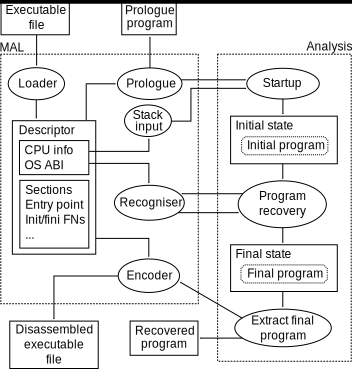
\includegraphics{./fig_schema}
\end{center}
\caption{The schema of the control-flow recovery in an executable file.}
\label{fig:schema}
\end{figure*}

The control-flow recovery process starts by passing the \emph{Executable file}
to the \emph{Microcode Abstraction Layer (MAL)} unit. It represents a software
layer allowing a control-flow recovery analysis (implemented in the unit
\emph{Analysis}) to analyse the \emph{Executable file} in term of the Microcode
platform (formally defined later in Section~\ref{sec:microcode}). The
\emph{Executable file} is processed by the module \emph{Loader}. It parses the
file and fills in the data storage \emph{Descriptor} with two types of
information:
\begin{enumerate}
\item A detected process architecture (CPU info) and operating system (OS ABI)
the executable file was built for. These data are stored into the upper box
inside the \emph{Descriptor}. %
\item An information about a content of the operational memory initialised
according to loadable sections in the executable file and dependent shared
libraries, if any. This information is stored into the  lower box inside the
\emph{Descriptor} %
\end{enumerate}
With respect to the second point the \emph{Loader} must understand how the
detected operating system loads executable files, in order to put data to right
addresses. Moreover, operating system also loads dependent shared libraries to
proper addresses, it performs address relocations, and possibly other things
related to the loading process. The \emph{Loader} must mimic all these thing,
because data stored in the \emph{Descriptor} have to represent the memory state
of all loaded sections right before the processor starts the execution at the
entry point to the loaded executable. Note though that the \emph{Descriptor}
holds only a description of how the memory is initialised, i.e. it describes a
mapping from addresses to concrete values.

Both kinds of data in the \emph{Descriptor} are then used by the module
\emph{Prologue} to build a Microcode program called \emph{Prologue program}.
This program (when executed) does three important things:
\begin{enumerate}
\item It allocates and initialises a content of the memory as described in the
descriptor (in the lower box). %
\item It allocates and initializes the stack. This especially includes reading
program arguments and environment variables and storing them to right places. %
\item It opens standard input and output streams.
\item It initialises all registers of the detected processor architecture so
that the execution of the loaded executable is just about to begin at the entry
point. In fact registers are modeled in a certain region of the memory in the
Microcode platform, so the program actually initialises that memory. %
\end{enumerate}
The \emph{Prologue program} is a Microcode program computing a memory content
which is \emph{equivalent} (bijective) to an initial state of a process created
from the \emph{Executable file} by the detected operating system running on the
detected processor architecture. %
Note though the same \emph{Executable file} can be started with different
program arguments and environment variables. This affects initial state of the
process's stack. A \emph{Prologue program} thus reads program arguments and
environment variables from standard input stream \#1 using ``Input \& Output"
instructions and sets up the stack according to received data. It means that it
is the unit \emph{Analysis} how is responsible to provide data from the stream.
In order to support this process the unit \emph{MAL} provides a module
\emph{Stack input} which generates a sequence of bytes of precisely defined
structure (see Section~\ref{sec:MAL:prologue} for details) representing a
default content of the input stream, i.e. a default initialisation of the stack.

Observe in the schema that the \emph{Prologue program} can be output to a user.
We consider it then as a secondary output. We will see it use later in
Section~\ref{sec:overview:chaining}.

%But primarily, the \emph{Prologue program} is passed to the \emph{Analysis} unit for
%construction of an initial state of a control-flow analysis.

Primarily, the \emph{Prologue program} is passed to %the module \emph{Startup}
% of
the unit \emph{Analysis}, together with an output from the module \emph{Stack
input}. This unit is responsible for the actual process of the control-flow
recovery in the analysed \emph{Executable file}. In general, an analysis starts
in some \emph{Initial state}. Its construction is performed in the module
\emph{Startup} by processing (e.g. executing) the accepted \emph{Prologue
program} with (possibly altered) data received from \emph{Stack input}. Although
we do not specify neither what information is stored in any state of the
analysis nor how it is organised, one think is certain: Since the only purpose
of the analysis is to build a Microcode program fully describing the
control-flow in the analysed \emph{Executable file}, this program must be
somehow encoded in states of the analysis. Therefore, we reflect this fact in
the schema by highlighting ``Initial program'' and ``Final program'' inside data
storages \emph{Initial state} and \emph{Final State} respectively. Of course,
the initial program should be empty as the analysis has no information about the
control flow in the \emph{Executable file} yet.

The module \emph{Program recovery} of the unit \emph{Analysis} plays the key
role in the schema as it performs the main computation in the recovery process
of the control-flow in the analysed \emph{Executable file}. The computation
starts with the \emph{Initial state} (accepted from the module \emph{Startup})
and then it computes any number of intermediate states until a final state with
a final Microcode program is not reached. This final state is then stored into
the data storage \emph{Final state}. The described computation could hardly be
performed without understanding effects of bytes in code sections of the
analysed \emph{Executable file}. Therefore, an important role in the computation
plays a communication with the module \emph{Recogniser} of the \emph{MAL} unit.
Simply said, the module \emph{Program recovery} may send a query to
\emph{Recogniser} to translate values of bytes at certain addresses into a
Microcode program having the same effect as an instruction of the detected
processor architecture (described in the upper box inside the data storage
\emph{Descriptor}) encoded at those bytes. \emph{Recogniser} then sends the
translated program back to the module \emph{Program recovery} as a response to
the query. For example, the execution of the \emph{Executable file} begins at
the entry point address to the executable. So, the \emph{Program recovery}
module may send a query to \emph{Recogniser} to translate the instruction
encoded in bytes starting at the entry address to an equivalent Microcode
program (i.e.~to a program having the same effect as the instruction). Then the
\emph{Program recovery} module may execute the received Microcode program to see
its effect on the memory and registers. The program also updates a value of the
\emph{instruction pointer} (IP) register such that it points to the first byte
of an instruction to be executed next. The \emph{Program recovery} module may
send another query to \emph{Recogniser} to translate the instruction at the
address stored in the updated IP into an equivalent Microcode program. The
program can then be executed and the process may continue further. We describe
the communication of both module in more details later in
Section~\ref{sec:MAL:recogniser}.

The final Microcode program can be encoded anyhow in the \emph{Final state}. So,
the module \emph{Extract final program} reads relevant information encoded in
the \emph{Final state} and builds the final program accordingly. This
computation can be more or less complex depending on how much the representation
of the program in the \emph{Final state} differs from the specification of a
Microcode program given in Section~\ref{sec:microcode}.

Observe in the schema the final Microcode program can be output to a user in the
form of the data storage \emph{Recovered program}. It is then considered as a
secondary output together with the \emph{Prologue program} discussed above.
These two programs together allow for chaining several control-flow recovery
analyses on the same \emph{Executable file}. We discuss this process in
Section~\ref{sec:overview:chaining}.

The final Microcode program, extracted from the \emph{Final state}, should
primarily be passed to the unit \emph{MAL}. Namely, to the module
\emph{Encoder}. It translates the accepted program into an equivalent assembler
program over instruction set of the detected processor architecture and
operating system (both described in the data storage \emph{Descriptor}). The
resulting assembly file, represented by the storage \emph{Disassembled
executable file}, is the primary output from the whole process of the
control-flow recovery in the \emph{Executable file}.


\subsection{Chaining of analyses}
\label{sec:overview:chaining}

Each control-flow recovery analysis has strengths and weaknesses. It performs
well on some executable files and purely for some others. It may thus happen in
the process described in the previous section that the resulting data storage
\emph{Disassembled executable file} holds an assembly program capturing only
some fraction of all control-flow in the analysed \emph{Executable file}. We may
then ask how to improve the result.

Here we propose a solution based on running several control-flow recovery
analyses in sequence for the same executable file. Each analysis in the sequence
(except the first one) is supposed to begin with the result of the preceding
analysis and it is supposed to extend it by finding some new (yet undiscovered)
control-flow in the executable. The first analysis computes a result from
scratch as we discussed in the previous section. We call this process as
\emph{chaining of analyses}.

Let as suppose we have a sequence $ A_1,\ldots,A_n $ of the length $ n $, where
each $ A_i $ represents some control-flow recovery analysis. It can be the case
that some analyses appears more than once in the sequence (i.e. there can be $ i
\ne j $ such that $ A_i = A_j $). On the other hand, it does not make any sense,
if two subsequent elements in the sequence represent the same analysis (i.e. for
all $ 0 < i < n $ we assume $ A_i \ne A_{i+1} $).

We run the analysis $ A_1 $ as we discussed in Section~\ref{sec:overview}, i.e
according to the schema depicted in the Figure~\ref{fig:schema}. There is one
difference thought. We do not need the primary output, i.e.~the
\emph{Disassembled executable file}. We only need the secondary output
represented by the data storages \emph{Prologue program} and \emph{Recovered
program}. So, to get the exact schema, we would have to remove form the
Figure~\ref{fig:schema} the module \emph{Encoder}, the data storage
\emph{Disassembled executable file}, and all arrows attached to them.

\begin{figure*}[!ht]
\begin{center}
\begin{tabular}{ccc}
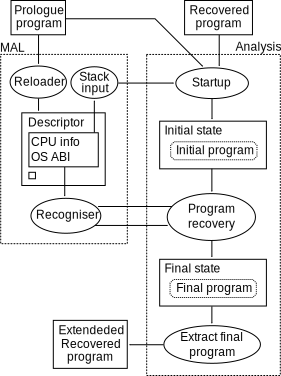
\includegraphics{./fig_schema_chaining}
& ~~~~~~~~~~~ &
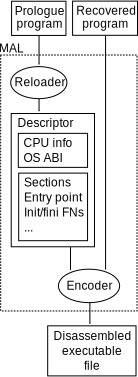
\includegraphics{./fig_schema_encoding}
\\ \\
(a) & & (b)
\end{tabular}
\end{center}
\caption{Chaining of control-flow recovery analyses. (a) An intermediate step.
(b) The final step.}
\label{fig:schema_chaining}
\end{figure*}

Next we run remaining analyses in the sequence one by one, each according to the
schema depicted in Figure~\ref{fig:schema_chaining}~(a). We see there the input
is represented by data storages \emph{Prologue program} and \emph{Recovered
program}, i.e.~by two Microcode programs. The \emph{Prologue program} was
generates during the run of the first analysis and it is not further modified.
It means that each subsequent analysis accepts the same \emph{Prologue program}.
On the other hand, the \emph{Recovered program} may change from one analysis to
another, because it is the output from the preceding analysis, represented in
the schema by the data storage \emph{Extended recovered program} (and by
\emph{Recovered program} in the Figure~\ref{fig:schema}) holding the resulting
Microcode program capturing (some part of) the control-flow in the analysed
\emph{Executable file} (passed to the first analysis of the sequence).

It is important to stress here that for each analysis in the sequence all input
and output Microcode programs (i.e. contents of data storages \emph{Prologue
program}, \emph{Recovered program}, and \emph{Extended recovered program}) are
always expressed as Microcode \emph{assembly files}, whose exact structure and
syntax is formally defined in Section~\ref{sec:microcode:assembly}. Therefore,
data passed to analyses along the sequence are expressed in the common format
understood by all of them.

Let us now follow the schema at Figure~\ref{fig:schema_chaining}~(a) to see how
the output program \emph{Extended recovered program} is computed from the input
programs \emph{Prologue program} and \emph{Recovered program} by some analysis $
A_i $, where $ 1 < i \leq n $.

We see the \emph{Prologue program} is passed to the module \emph{Reloader} of
the \emph{MAL} unit. This module is an equivalent of the \emph{Loader} module of
the schema at the Figure~\ref{fig:schema}. So, its purpose is to fill in the
data storage \emph{Descriptor} with the information about the processor
architecture and operating system the \emph{Executable file} was build for,
together with the description of the initial content of the operational memory
related to loadable sections in the \emph{Executable file} and dependent shared
libraries, if any. But in contrast to \emph{Loader} who parses the information
directly from the executable file, the \emph{Reloader} collects the same
information from the \emph{Prologue program}. Observe in the schema that the
lower box inside the \emph{Descriptor} is depicted only by the small rectangle.
That indicates that it is actually not used in the schema. Indeed, it has to
store only information needed by the module \emph{Recogniser}, i.e.~the
information about the processor architecture and the operating system (the upper
box). This gives us an opportunity to speed up the \emph{Reloader}, when it is
used in this context. Nevertheless, it must be able to fully reconstruct the
\emph{Descriptor} when it is used in the context of the schema at
Figure~\ref{fig:schema_chaining}~(b), which we will discuss later.

The \emph{Prologue program} is also passed to the module \emph{Startup} of the
\emph{Analysis} unit together with the \emph{Recovered program} (i.e.~with the
output from the preceding analysis). Moreover, since an execution of the
\emph{Prologue program} always reads information about command line arguments
and environment variables from the standard input stream \#1, the module
\emph{Startup} also accepts a default version of these data from the module
\emph{Stack input}. The \emph{Startup} is supposed to build the \emph{Initial
state} of the analysis the same way as we discussed in the previous section for
the same module in Figure~\ref{fig:schema}. The only difference is that the
initial program encoded in the state is not empty now, but it is the accepter
\emph{Recovered program}.

Remaining modules of the schema work exactly the same ways as the corresponding
modules in the schema at Figure~\ref{fig:schema}, see previous section for
details.

As the final step we translate the result from the last analysis in the
sequence, i.e.~the last \emph{Extended recovered program}, into an equivalent
assembler program over instruction set of the processor architecture and
operating system remembered in the \emph{Prologue program}. This process is
depicted by the schema at Figure~\ref{fig:schema_chaining}~(b).

Observe that the \emph{Prologue program} is passed to the module \emph{Reloader}
of the unit \emph{MAL} in order to fully reload the \emph{Descriptor} with all
relevant information stored in the \emph{Prologue program}. It means that the
\emph{Descriptor} will hold the same information it held when running the first
analysis in the sequence, i.e.~according to the (updated) schema at
Figure~\ref{fig:schema}. The module \emph{Encoder} then applied the same
computation on the accepted \emph{Recovered program} as we discussed in the
previous section for this module.

\paragraph{Open questions} %
The following two questions are tightly related to the discussed topic. Although
they are important and interesting, their answering is beyond the scope of this
paper.
\begin{itemize}
\item  Given a total analysis time, how long the sequence of analyses should be
and what subset of all available analyses we should consider for building the
sequence? %
\item How should we split the total analysis time amongst individual analyses in
the sequence? %
\end{itemize}

In the next section we provide a specification of the Microcode platform. Then,
in Section~\ref{sec:MAL}, we specify a mandatory features and
properties of the Microcode abstraction layer. It also includes the description
of the interface used in the communication between units \emph{MAL} and
\emph{Analysis}. 


\section{Microcode platform}
\label{sec:microcode}

Microcode platform is an abstract computational model. It defines a structure of
the operational \emph{memory}, a Microcode \emph{program}, and its
\emph{execution}. The memory consists of three disjoint memory pools, each with
a particular purpose. A program is a directed graph whose edges are labeled by
\emph{instructions}. Each instruction has a particular effect on the program's
execution and on contents of the memory pools. A program does \emph{not} reside
in the memory. During its execution it may access the memory (read and/or
write), but it can \emph{not} access itself. It means the program cannot be
neither read nor written by its instructions. There can be executed at most one
program at time on this platform. Nevertheless, the program can spawn any number
of \emph{threads}.

We describe the structure of the operational memory in
Section~\ref{sec:microcode:memory}. Then we define a Microcode program in
Section~\ref{sec:microcode:program} and its execution in
Section~\ref{sec:microcode:execution}. A complete list of all instructions
together with their detailed description is given in
Section~\ref{sec:microcode:instructions}. Since it is further convenient to
present a given program to a human in a textual form, we also define a structure
of an \emph{assembly} text of the program in
Section~\ref{sec:microcode:assembly}.


\subsection{Memory}
\label{sec:microcode:memory}

The memory of the Microcode platform consists of three disjoint memory pools
\texttt{REG}, \texttt{MEM}, and \texttt{SYS}. First two are arrays of $ 2^{64} $
bytes indexed (addressed) from zero. An underlying data structure of
\texttt{SYS} memory pool is not specified.

\subsubsection{\texttt{REG} pool}
\label{sec:microcode:memory:REG}

It holds a complete information about a state of a certain a priori given
processor architecture (like x86) and it also provides a space for storing
intermediate results of an executed program.

By the complete information of a processor we mean contents of all its
registers, including flags and states of built-in co-processors (like FPU x87).
We do not specify, how the information is stored in the pool (i.e. where is
mapped which register or flag) and in how many bytes the information is encoded.
It is defined by a Microcode abstraction layer, discussed in
Section~\ref{sec:MAL}. The encoding may differ from one processor
architecture to another. Nevertheless, it must always be the case the processor
state is mapped from the beginning of the pool (i.e.~from the address 0) up to
some arbitrarily chosen but then fixed address \texttt{tmp}. Also the
\emph{instruction pointer} (IP) register of the processor architecture must
always be mapped into the address range $ [0,8) $ (i.e.~addresses 0,\ldots,7)
starting at the address 0. Other registers are mapped from the address 8 on. We
denote the range $ [0,\texttt{tmp}) $ of this pool as the \emph{memory for
registers}.

The remaining bytes of the pool, i.e. those in the range $ [\texttt{tmp},2^{64})
$, can be used arbitrarily, for any purpose. This memory is typically used by a
program during its execution for storing intermediate results of its
computation. We thus denote this range of addresses of the pool as the
\emph{memory for temporary variables}.

Numbers stored in the whole pool are assumed to be in the big endian. We express
a content of the pool by a function $ \mathit{reg}: \{ 0, \ldots, 2^{64}-1 \}
\rightarrow \{ 0, \ldots, 2^{8}-1 \}$.

%For example, for a x86\_64 CPU the register
%\texttt{rax} can be mapped to the range [8,16), \texttt{eax} to [12,16),
%\texttt{ah} to [14,15), \texttt{al} to [15,16), \texttt{rbx} to [16,24), and so
%on.

\subsubsection{\texttt{MEM} pool}
\label{sec:microcode:memory:MEM}

It represents the physical operational memory (RAM) of a certain a priori given
processor architecture (like x86). Its purpose is to store all data and code of
a process created from a given executable file by a certain operating system
(like Linux) running on that processor architecture. The layout of data in this
pool are supposed to match the layout of the data in the (virtual) address space
of the created process.

We do not specify endianness of this pool. In general, different endianness can
be associated with different regions in the pool and the it may change during
execution of a program. We express a content of the whole pool by a function $
\mathit{mem}: \{ 0, \ldots, 2^{64}-1 \} \rightarrow \{ 0, \ldots, 2^{8}-1 \}$.

\subsubsection{\texttt{SYS} pool}
\label{sec:microcode:memory:SYS}

It holds the following information:
\begin{itemize}

\item What addresses in the \texttt{MEM} pool are accessible by instructions of
an executed Microcode program with what permissions. Access permissions of an
address in a subset of $ \{ \mathit{read}, \mathit{write}, \mathit{execute} \}
$.

\item An assignment of processor interrupts and exceptions (like ``division by
zero'', ``memory segmentation fault'', ``not an instruction'') of a certain a
priori given processor architecture (like x86) to values of the instruction
pointer register (i.e.~values in the range $ [0,8) $ in the \texttt{REG} pool)
where in the \texttt{MEM} pool are located routines responding to those
interrupts and exceptions.

\end{itemize}
We do not specify how the information is held in this pool. Typically, it is a
collection of data structures like dictionaries, arrays, etc. We use a symbol
\textit{sys} to reference a content of the pool.

\paragraph{Note} In all three pools there we consider some priori given
processor architecture. It is forbidden to consider different processor
architectures in different pools.

\subsection{Program}
\label{sec:microcode:program}

A \emph{program} is a finite \emph{directed graph}. Nodes represent points in
the computation (i.e. they allow us to say where we are in the computation) and
edges represent possible transitions between them. Each edge is labeled by an
\emph{instruction} specifying an action to be performed when moving from the
source node to the target one. Any node may have the out-degree at most 2. When
a node has the out-degree 2, then it is called \emph{branching}, its out-edges
have different target nodes (we disallow parallel edges), and they are labeled
by the complementary guard instructions (see Table~\ref{tab:igroup:guards} of
the Section~\ref{sec:microcode:instructions}). Any program may have at most $
2^{64} $ nodes and at most $ 2^{64} $ edges. We identify nodes by unique
identifiers, i.e. by numbers from the set $ \{ 0, \ldots, 2^{64}-1 \} $.
Formally, we define a map $ \mathit{id} $ from nodes to their unique
identifiers. In the text we do not distinguish between nodes and their
identifiers.

Each program consists of one or more \emph{components}. Each component has one
node marked as the \emph{entry} node. All nodes of a component must be
graph-reachable from the entry node. Each node with the out-degree 0 is called
an \emph{exit} node from the component. One component of a program is marked as
the \emph{start} component.

A program does \emph{not} lie in the memory, i.e.~it is \emph{not} stored in the
memory pools \texttt{REG}, \texttt{MEM}, \texttt{SYS}. You can imagine it
appears in some other unspecified memory pool. Instructions of a program may
have an effect on its execution. In particular, they may access (read and/or
write) contents of memory pools \texttt{REG}, \texttt{MEM}, and \texttt{SYS}. On
the other hand, an instruction can \emph{not} access the program itself, i.e. it
cannot read nor write (modify) the program.

We present an example program statically allocating 20 bytes in \texttt{MEM},
initialising the fist 10 bytes of the memory and then copying those bytes into
the remaining 10 bytes is depicted at Figure~\ref{fig:copy_program}~(a). Note
that identifiers of nodes can optionally be drawn inside the nodes. The
structure and meaning of instructions is defined later in
Section~\ref{sec:microcode:instructions}.


\subsubsection{Program API}
\label{sec:microcode:programAPI}

Any implementation of Microcode's program must provide a public read access to
the following properties of the program:
\begin{itemize}
\item The number of components the program consists of. Each component is
associated with a unique ordinal from the set $ \{ 0, \ldots, n-1 \} $, where $
n $ is the number of components. The start component is always associated with
the ordinal 0.

\item For each component, identified by its ordinal, there must be a public read
access to the following its properties:
\begin{itemize}
\item The identifier of the entry node.

\item The number of exit nodes. Each exit node is associated with a unique
ordinal from the set $ \{ 0, \ldots, n-1 \} $, where $ n $ is the number of exit
nodes.

\item The identifier of an exit node referenced by its ordinal.

\item The in-degree of a node referenced by its identifier. Each in-edge of the
node is associated with a unique ordinal from the set $ \{ 0, \ldots, n-1 \} $,
where $ n $ is the in-degree of the node.

\item The identifier of the source node of an in-edge to a given target node.
The target node is referenced by its identifier and the in-edge by its ordinal.

\item The out-degree of a node referenced by its identifier. Each out-edge of the
node is associated with a unique ordinal from the set $ \{ 0, \ldots, n-1 \} $,
where $ n $ is the out-degree of the node.

\item The identifier of the target node of an out-edge to a given source node.
The source node is referenced by its identifier and the out-edge by its ordinal.

\item A reference to the instruction labeling a given edge referenced by
identifiers of its source and target node. It must be the case the edge belongs
to in-edges of the target node and to out-edges of the source node.
\end{itemize}
\end{itemize}

The type of returned identifiers of nodes and all mentioned ordinals must be
unsigned integers of fixed sizes 8, 16, 32, or 64 bits long big enough to
capture associated properties of the program. The type of a reference to an
instruction is not specified.

\subsection{Execution}
\label{sec:microcode:execution}

A \emph{thread} in a given program is a triple $
(\mathit{id},\mathit{stack},\mathit{reg}) $, where \textit{id} is a number from
the set $ \{ 0, \ldots, 2^{64}-1 \} $ distinguishing the thread from all others,
\textit{stack} is a non-empty LIFO data type storing (identifiers of) program's
nodes, e.g. $ [n_1,\ldots,n_k] $ is a stack of $ k $ program's nodes with $ n_k
$ on the top, and $ \mathit{reg} $ defines the content of the \texttt{REG}
memory pool.

%An \emph{execution of an instruction} of a given program over contents $
%\mathit{reg} $, $ \mathit{mem} $, and $ \mathit{sys} $ of the memory pools
%\texttt{REG}, \texttt{MEM}, and \texttt{SYS} respectively is a new content $
%\mathit{reg}' $ of the \texttt{REG} pool and possibly updated contents $
%\mathit{mem} $ and $ \mathit{sys} $, all according to semantics of the
%instruction as defined in Sec.~\ref{sec:microcode:instructions}. We assume that
%initial contents $ \mathit{reg} $, $ \mathit{mem} $, and $ \mathit{sys} $
%satisfy all preconditions of the executed instruction so that its execution
%cannot fail. Wherever necessary, checking for assumptions must be explicitly
%present in the program, i.e. there must be additional (safety) edges in the
%program preceding an instruction whose execution may fail and preventing failure
%of its execution. Any attempt to execute an instruction on contents $
%\mathit{reg} $, $ \mathit{mem} $, and $ \mathit{sys} $ not matching
%preconditions of the instruction lead to an undefined behaviour of the whole
%program.

%An \emph{execution step} of a thread $
%(\mathit{id},[n_1,\ldots,n_k],\mathit{reg}) $ over contents $ \mathit{mem} $ and
%$ \mathit{sys} $ of the memory pools \texttt{MEM} and \texttt{SYS} respectively
%is a set of threads $ T' $ of the size at most 2 and possible updates of $
%\mathit{mem} $ and/or $ \mathit{sys} $.

\begin{algorithm*}[!t]

\caption{ An execution of a program over $ \mathit{mem} $ and $ \mathit{sys} $. }
\label{alg:execution}

\KwIn{A program, maps $ \mathit{reg} $ and $ \mathit{mem} $ defining an
initial content of \texttt{REG} and \texttt{MEM} pools, and an initial content $
\mathit{sys} $ of the \texttt{SYS} pool. }

\BlankLine

$ T $ := $ \{ (0,[e],\mathit{reg}) \} $~~~~\textit{// '$ e $' is the entry node
of the start component.}
\label{alg:execution:mainThread}

\Repeat{
$ T = \emptyset$~~~~\textit{// Exit the loop when there is no thread in $ T $.}
\label{alg:execution:normalTermination}
}{
$ W $ := choose (e.g.~randomly) a non-empty subset of $ T $.
\label{alg:execution:chooseW}

$ T $ := $ T \setminus W $

$ W_d $ := $ \emptyset $

$ R_d $ := $ \emptyset $

$ W_c $ := $ \emptyset $

$ R_c $ := $ \emptyset $

\ForEach{
$ t \in W $~~\textit{/* Enumerate threads in $ W $ in some order (e.g.~randomly). */}
\label{alg:execution:enumerateW}
}{

$ T' $ := perform the execution step of $ t $ over $ \mathit{mem} $ and $
\mathit{sys} $~~\textit{// It may produce 0,1, or 2 threads.}
\label{alg:execution:step}

\If{\rm execution step of $ t $ has failed due to its undefined behaviour}{
 \textbf{STOP}~\textit{// Undefined
behaviour: The precondition of an executed instruction is not satisfied.}
\label{alg:execution:terminateInstruction} }

$ W_{d}' $ := $ \{~a~;~\mathit{mem}(a)$ was written by a ``Data transfer''
instruction in the execution step of $ t~\} $

$ R_{d}' $ := $ \{~a~;~\mathit{mem}(a)$ was read by a ``Data transfer'' instruction in the execution step of $ t~\} $

$ W_{c}' $ := $ \{~a~;~\mathit{mem}(a)$ was written by a ``Concurrency''
instruction in the execution step of $ t~\} $

$ R_{c}' $ := $ \{~a~;~\mathit{mem}(a)$ was read by a ``Concurrency''
instruction in the execution step of $ t~\} $

\If{$ (W_{d} \cap (W_{d}' \cup R_{d}' \cup W_{c}' \cup R_{c}')) \cup
  (R_{d} \cap (W_{d}' \cup W_{c}')) \cup
  (W_{c} \cap (W_{d}' \cup R_{d}')) \cup
  (R_{c} \cap W_{d}') \not= \emptyset $
\label{alg:execution:illegal_concurrency}
}{ \textbf{STOP}~\textit{// Undefined behaviour:
Illegal concurrent access to the same address by threads. }
\label{alg:execution:race} }

$ W_d $ := $ W_d \cup W_d' $

$ R_d $ := $ R_d \cup R_d' $

$ W_c $ := $ W_c \cup W_c' $

$ R_c $ := $ R_c \cup R_c' $

$ T $ := $ T \cup T' $
}

}

\end{algorithm*}

An \emph{execution step} of a thread $
(\mathit{id},[n_1,\ldots,n_k],\mathit{reg}) $ over contents $ \mathit{mem} $ and
$ \mathit{sys} $ is a process computing a set of threads $ T' $ of the size at
most 2 with possible updates of contents $ \mathit{mem} $ and $ \mathit{sys} $.
In this process all out-edges of $ n_k $ are considered and effects of their
instructions are computed and properly used. Many instruction are associated
with conditions which must be satisfied for their correct execution. We call
them \emph{preconditions} of instructions. Execution of an instruction fails, if
its precondition is not satisfied. Neither behaviour nor result of the execution
step is then defined. We speak about \emph{undefined behaviour} of the execution
step. Next we enumerate all cases which may occur during execution step of a
thread. In each case we present structure of threads in $ T' $ and we also
mention whether contents $ \mathit{mem} $ and $ \mathit{sys} $ are updated or
not. On the other hand we do not specify how the contents $ \mathit{mem} $, $
\mathit{sys} $, and contents $ \mathit{reg} $ of individual threads in $ T' $
were concretely updated. We discuss it later in
Sec.~\ref{sec:microcode:instructions}. Here are the possible cases:
\begin{itemize}

\item If $ k = 1 $ and $ n_k $ is an exit node of some component of the program,
then $ T' $ is empty and $ \mathit{mem},\mathit{sys} $ are not changed.

\item If $ k > 1 $ and $ n_k $ is an exit node of some component of the program,
then $ T' = \{ (\mathit{id},[n_1,\ldots,n_{k-1}],\mathit{reg}) \} $ and $
\mathit{mem},\mathit{sys} $ are not changed.

\item If the out-degree of $ n_k $ is 1 and the only out-edge $ (n_k, n_k') $
form $ n_k $ is labeled by a \texttt{CALL} instruction (see
Table~\ref{tab:igroup:modularity}) referencing an entry node $ e $ of some
component, then $ T' = \{ (\mathit{id},$  $[n_1,\ldots,n_{k-1},n_k',e],$ 
$\mathit{reg}) \} $ and $ \mathit{mem},\mathit{sys} $ are not changed.

\item If the out-degree of $ n_k $ is 1 and the only out-edge $ (n_k, n_k') $
form $ n_k $ is labeled by a \texttt{THREAD} instruction (see
Table~\ref{tab:igroup:concurrency}, SID=0), then $ T' = \{
(\mathit{id},[n_1,\ldots,n_{k-1},n_k'],$  $\mathit{reg}'),
(\mathit{id}',$  $[n_1,\ldots,n_{k-1},n_k'],\mathit{reg}'') \} $, where $ \mathit{id}' $ is
fresh, i.e. there is no other thread in the program with $ \mathit{id}' $, $
\mathit{reg}' $ and $ \mathit{reg}'' $ represent an effect of the instruction's
execution on $ \mathit{reg} $. Contents $ \mathit{mem} $ and $ \mathit{sys} $
are not changed.

\item If the out-degree of $ n_k $ is 2, then out-edges from $ n_k $ are labeled
by complementary guard instructions (see Table~\ref{tab:igroup:guards}). Let $
(n_k, n_k') $ be the only out-edge whose guard executes (evaluates) to
\textit{true}. Then $ T' = \{ (\mathit{id},[n_1,\ldots,n_{k-1},n_k'],$ $\mathit{reg}) \}
$ and $ \mathit{mem},\mathit{sys} $ are not changed.

\item Otherwise, $ T' = \{ (\mathit{id},[n_1,\ldots,n_{k-1},n_k'], \mathit{reg}') \} $,
where $ n_k' $ is the target node of the only out-edge from $ n_k $, $
\mathit{reg}' $ represent an effect of execution of the instruction labeling the
edge $ (n_k,n_k') $. $ \mathit{mem} $ and $ \mathit{sys} $ may also be
updated by the instruction's execution.

\end{itemize}

An \emph{execution} of a program over contents $ \mathit{mem} $ and $
\mathit{sys} $ is defined in Algorithm~\ref{alg:execution}. It begins with a
single thread started at the entry node of the start component (see
line~\ref{alg:execution:mainThread}). Executions steps are then performed on
this thread and later possibly on other threads created during the execution
(see line~\ref{alg:execution:step}). The execution finishes when there is no
thread for which to perform execution step (i.e. the set $ T $ becomes empty,
see line~\ref{alg:execution:normalTermination}), or some thread executes an
instruction whose precondition is not satisfied (see
line~\ref{alg:execution:terminateInstruction}), or when instructions executed by
two or more concurrently executed threads (i.e.~those in the set $ W $) perform
a prohibited concurrent access (read/write) to the content \textit{mem} (see
line~\ref{alg:execution:race}). Accesses to \textit{mem} are logged in sets $
W_d, R_d, W_c, R_c, W_d', R_d', W_c' $, and $ R_c' $, and the condition defining
an illegal concurrent access is presented at
line~\ref{alg:execution:illegal_concurrency}. The condition can be more easily
understand using the table bellow, where the value 1 indicates a wrong memory
access when the intersection of the corresponding non-primed and primed set (in
the heading of the row and the column respectively) is a non-empty set:
\begin{center}
\begin{tabular}{c|cccc}
         & $ W_d' $ & $ R_d' $ & $ W_c' $ & $ R_c' $ \\\hline
$ W_d $  &    1     &    1     &    1     &    1     \\
$ R_d $  &    1     &    0     &    1     &    0     \\
$ W_c $  &    1     &    1     &\textbf{0}&\textbf{0}\\
$ R_c $  &    1     &    0     &\textbf{0}&\textbf{0}\\
\end{tabular}
\end{center}
The condition at line~\ref{alg:execution:illegal_concurrency} was constructed
per rows of the table. For example, the second term $ R_{d} \cap (W_{d}' \cup
W_{c}') $ in the condition corresponds to the second row in the table: The
memory access is illegal when $ R_{d} \cap W_{d}' $ or $ R_{d} \cap W_{c}' $ is
a non-empty set, which is equivalent to $ R_{d} \cap (W_{d}' \cup W_{c}') $
being non-empty. Note that bold zeros in the table indicate that intersection of
the corresponding sets is always empty (see ``test and set'' instructions in
Table~\ref{tab:igroup:concurrency}).

Observe further in the algorithm that parallel execution of threads is simulated
by the choice of the subset $ W $ at line~\ref{alg:execution:chooseW}. And an
order in which threads access to synchronisation variables (see ``test and set''
instructions in Table~\ref{tab:igroup:concurrency}) is modeled
line~\ref{alg:execution:enumerateW} by choosing a particular enumeration order
of threads in $ W $.


\subsection{Instruction set}
\label{sec:microcode:instructions}

We already know that a Microcode instruction is a label of an edge $ (n_k,n_k')
$ defining an effect of an execution step of a current thread $
(\textit{id},[n_0,\ldots,n_k],\mathit{reg} ) $ to contents $ \mathit{mem} $, and
$ \mathit{sys} $, and to $ \mathit{reg} $ contents of resulting threads. In this
section we list all instructions with descriptions of their execution effects on
the mentioned contents. Moreover, for each instruction whose execution may fail
we provide a \emph{precondition}, i.e.~a weakest necessary condition for
executing the instruction without any failure.

We sort instructions to logical \emph{groups} according to similarities in their
execution effects. We further sort instructions in each group into
\emph{subgroups} by types of their formal parameters and operators used, if any.
Each instruction is then uniquely identified by a unique \emph{group identifier}
(GID) and \emph{subgroup identifier} (SID). A subgroup identifier is unique only
inside its group. Finally, we define a \emph{global instructing kind} (GIK) as
the addition of GID and SID identifiers of an instruction.

In Tables~\ref{tab:igroup:guards}-\ref{tab:igroup:miscellaneous} we present
individual group of instructions. In each table we define GID (inside the
caption) and all instruction subgroups. Since instructions of many subgroups
accept arguments, we list them in the exact and mandatory order. We write
arguments in italic. We use the following naming convention (symbols) for
arguments:
\begin{itemize}

\item $ a $, $ a' $, $ a'' $, and $ a''' $ : Symbols for addresses to either
\textit{reg} or \textit{mem} contents. An address is a big-endian 64-bit
unsigned integer. Whenever any of these symbols appears in a range, then we
assume each address in the range is less than $ 2^{64} $. For example, if $ a $
is used in a range $ [a,a+k) $, then we assume $ a \leq 2^{64}-k $.

\item $ v_{b} $,  $ v_{b}^0 $,  $ v_{b}^1, \ldots $ : Symbols for $ 8b $-bits
long big-endian binary representations of values of unsigned integers.

\item $ m $,  $ m' $, $ n, n' $, and $ n'' $ : Any numbers from sets $ \{ 1,2,4
\} $, $ \{ 4,8 \} $, $ \{ 1,2,4,8 \} $, $ \{ 1,2,4,8 \} $, and $ \{
1,2,4,8,16 \} $  respectively.

\item $ f $ : $ 80 $-bits long IEEE 754 floating point number which is
\emph{not} \texttt{NaN}.

%\item $ w $ : Any positive integer.

%\item $ e $ : An identifier of the entry node of some component of an analysed
%program.

%\item $ r $ : A triple of bits (\texttt{READ},\texttt{WRITE},\texttt{EXECUTE})
%defining access rights for allocated memory blocks. It is thus an integer in $
%\{ 0,\ldots,7\} $.

\end{itemize}

For each subgroup we also present textual representations of instructions, i.e.
assembly texts. They are all case sensitive and arguments are encoded as either
decimal or hexadecimal unsigned integer literals, except the argument $ f $
which is encoded as a floating point literal as in C language. Hexadecimal
unsigned integers must be typed in lower-case and terminated by 'h'.

We restrict a set of instructions which may write into address range $ [0,8) $
in \texttt{REG} pool to the following, where $ a $ and $ v $ are any 64-bit unsigned
integers:
\begin{center}
\begin{tabular}{cl}
\textbf{GIK} & \textbf{Assembly text}
\\
%\hline
2+0 & \texttt{REG[0]\{8\} := }$ v $\texttt{\{8\}}\\
2+1 & \texttt{REG[0]\{8\} := REG[}$ a $\texttt{]\{8\}}\\
36+0 & \texttt{REG[0]\{8\} := REG[0]\{8\} +\{8\} }$ v $\texttt{\{8\}}\\
36+1 & \texttt{REG[0]\{8\} := REG[0]\{8\} +\{8\} REG[}$ a $\texttt{]\{8\}}\\
\end{tabular}
\end{center}

\noindent Moreover, execution of subsequent instructions must be independent of
the current content of the \texttt{REG} pool in the range $
[\texttt{tmp},2^{64}) $. In other words, no matter what changes we perform in
that range the subsequent execution will always proceed exactly the same way.

\subsubsection{Instruction API}
\label{sec:microcode:instructionAPI}

Any implementation of Microcode's instruction set must provide for any
instruction (accessed through a reference in the program, see
Section~\ref{sec:microcode:programAPI}) a public read access to its GID, SID,
and all its arguments. Individual arguments are identified by their ordinals in
the list of arguments. The first argument has the ordinal 0. For example,
arguments list of an instruction with GID=2 and SID=0 is [$ n $, $ a $, $ v_n $]
(see Table~\ref{tab:igroup:setandcopy}), so the argument 0 is $ n $, the
argument 1 is $ a $, and the argument 2 is $ v_n $.

GID and SID identifiers must be returned as 8-bit unsigned integers. The number
of arguments must be a 64-bit unsigned integer. For each argument there must be
a available its size in bytes -- an 8-bit unsigned integer. An access to a value
of an argument must be provided via an address to its first byte. There the
value is stored as an unsigned integer number or as $ 80 $-bits long IEEE 754
floating point number, if the argument represents a floating point number. The
number is stored in endian of the platform on which the module is compiled.



% % % % % % % % % % % % % % % % % % % % % % % % % % % % % % % % % % % % % % % % %
% % % % % % % % % % % % % % % % % % % % % % % % % % % % % % % % % % % % % % % % %


\subsection{Textual program representation}
\label{sec:microcode:assembly}

Here we specify, how a given program can be represented as a plain text, i.e.~as
an \emph{assembly file}. Since the program is a directed graph, we basically
specify how to store the graph as a text. This can be done many ways. We focus
on easy readability for a human.

We represent a program as a sequence of case-sensitive text lines. There are
four types of lines:
\begin{itemize}
\item \emph{Instruction line} : A line containing the assembly text of a single
instruction, possibly surrounded by any number of white-space characters. The
structure of assembly texts of individual instructions were already specified in
Section~\ref{sec:microcode:instructions}. We assume there is a map $ T $ from
instructions to their assembly texts.%

\item \emph{Label line} : It is a line with one of the following three possible
types of content, possibly surrounded by any number of white-space characters:
`\texttt{@}$ X $', `\texttt{@}$ X $\texttt{:}', or `\texttt{@}$ X $ $ T(G) $
\texttt{@}$ Y $', where the symbols $ X $ and $ Y $ stand for any non-empty
string literals over alpha-numeric characters and the underscore, and the symbol
$ G $ stands for any guard instruction (see Table~\ref{tab:igroup:guards}). For
any $ X $ there can be at most one label line of the form `\texttt{@}$ X
$\texttt{:}' in an assembly file. We call symbols $ X $ and $ Y $ as \emph{label
names}. %

\item \emph{Annotation line} : It is a line containing a text of the form
`\texttt{\#}$ K $\texttt{:}$ B $' possibly surrounded by any number of
white-space characters, where $ K $ is any non-empty string literal over
alpha-numeric characters, the underscore, and the dot, and $ B $ is be any
string literal, even empty one. We call $ K $ as \emph{keyword} of the
annotation and we call the string literal $ B $ as \emph{body} of the
annotation. A syntactical structure and meaning of the body $ B $ is determined
by the keyword $ K $ of the annotation. Annotations do \emph{not} provide any
information about the structure of the encoded program. It is completely given
by instruction lines and label lines. Annotation lines allow for insertion into
the assembly file some additional information related to the encoded program in
a standardised way so that it can possibly be reused in the schema of chaining
of analyses presented in Section~\ref{sec:overview:chaining}. We discuss
annotations separately in Section~\ref{sec:microcode:assembly:annotations}.

%

\item \emph{Empty line} : It consists of any number of white-space characters. This
line carries no information about the graph. %
\end{itemize}
Each line (of any type) is terminated either by the character
`\texttt{\textbackslash n}', or by a pair of characters `\texttt{\textbackslash
r}\texttt{\textbackslash n}', or by the string literal `\texttt{//}'. In the
last case all subsequent characters are ignored up to the first occurrence of
any of the other two line terminators (i.e.~`\texttt{\textbackslash n}' or
`\texttt{\textbackslash r}\texttt{\textbackslash n}'). If a line terminator
`\texttt{\textbackslash n}' or `\texttt{\textbackslash r}\texttt{\textbackslash
n}' is directly preceded by the character `\textbackslash\textbackslash'
(backslash) then both `\textbackslash\textbackslash' and the terminator are
ignored and the line continues after the terminator further.

We use label lines to reflect connectivity of the graph in the assembly file.
Any pair of label lines of the form `\texttt{@}$ X $' and `\texttt{@}$ X
$\texttt{:}' with the same label name $ X $ represents a flow of control in the
assembly file from the line `\texttt{@}$ X $' to the line `\texttt{@}$ X
$\texttt{:}'. A label line of the form `\texttt{@}$ X $ $ T(G) $ \texttt{@}$ Y
$' allows for branching in the assembly file. If $ G $ is satisfied, then the
control in the assembly file flows to the label line `\texttt{@}$ X
$\texttt{:}', and to the label line `\texttt{@}$ Y $\texttt{:}' otherwise. The
label lines `\texttt{@}$ X $\texttt{:}' and `\texttt{@}$ Y $\texttt{:}' may
appear anywhere in the assembly file. The control flows from an instruction line
or from a label line of a form `\texttt{@}$ X $\texttt{:}' to the closest
subsequent instruction or label line of a form `\texttt{@}$ X $' in the file.
Annotation lines and empty lines are ignored in this context. Finally, we
distinguish a special label line \texttt{@EXIT} whose successor line is
undefined.

\subsubsection{Encoding program to assembly file}
\label{sec:microcode:assembly:encoding}

First, we create a function $ L $ from all nodes of the graph to label names
such that the entry node of the start component is mapped the name
\texttt{ENTRY}, all exit nodes (from all components) are mapped to the same name
\texttt{EXIT}, and all remaining nodes are mapped to pairwise different label
names other than \texttt{ENTRY} and \texttt{EXIT}. For example, we can define $
L $ as the map $ \mathit{id} $ for those remaining nodes.

We further augment the map $ T $ from instructions to their assembly texts for
modularity instructions (see Table~\ref{tab:igroup:modularity}) such that for
each entry node $ u $ to a component we have $ T(\texttt{CALL } \mathit{id}(u))
= \texttt{CALL } L(u)$.

 Then, we encode each
pair of edges $ (u,v) $ and $ (u,w) $ with a guard instruction $ G $ labeling $
(u,v) $ by 2 subsequent lines: `\texttt{@}$ L(u) $\texttt{:}' and `\texttt{@}$
L(v) $~~$ T(G) $~~\texttt{@}$ L(w) $'. Any other edge $ (u,v) $ labeled by a
non-guard instruction $ I $ is encoded by 3 subsequent lines: `\texttt{@}$ L(u)
$\texttt{:}', `$ T(I) $', and `\texttt{@}$ L(v) $'.

We do not specify in what order pairs and triples of lines (generated for
individual edges as described above) are stored in the file. But once some order
is chosen, then we apply the following post-process step. We remove from the
file each pair of subsequent lines of the form: `\texttt{@}\textit{X}' and
`\texttt{@}$ X $:', where $ X $ is any label name appearing both lines and $ X
\ne $ \texttt{ENTRY}, $ X \ne $ \texttt{EXIT}, and $ L^{-1}(X) $ does not appear
in any call instruction in the program.

As an optional final step we may insert of any sequence of empty and annotation
lines in front of any instruction line or any label line of the form
`\texttt{@}$ L(v) $~~$ T(G) $~~\texttt{@}$ L(w) $' or `\texttt{@EXIT}'.

The described process represents a set of all correct assembly texts of a given
program. A concrete implementation may produce any of them using any algorithm.

\begin{figure*}[!ht]
\begin{center}
\begin{tabular}{c|c}
\hspace{-1cm}
\begin{tabular}{c}
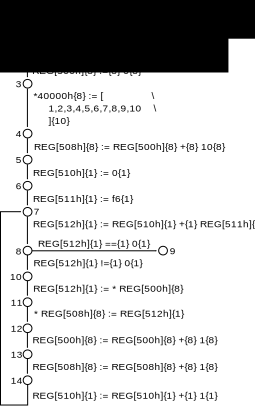
\includegraphics{./fig_copy_program}
\end{tabular} &
\begin{tabular}{l}
\texttt{@data:}\\
\texttt{~~~~*40000h\{8\} := [ ~~\textbackslash}\\
\texttt{~~~~~~~~1,2,3,4,5,~~~~\textbackslash}\\
\texttt{~~~~~~~~6,7,8,9,10~~~~\textbackslash}\\
\texttt{~~~~]\{10\}}\\
\texttt{~~~~@EXIT}\\\\\\
\texttt{@ENTRY:}\\
\texttt{~~~~REG[500h]\{8\} := MEM STATIC 3\{1\}, 20\{8\}, \textbackslash}\\
\texttt{~~~~~~~~~~~~~~~~~~~~40000h\{8\}}\\
\texttt{~~~~@init REG[500h]\{8\} !=\{8\} 0\{8\} @EXIT}\\
\texttt{@init:}\\
\texttt{~~~~CALL data}\\
\texttt{~~~~REG[508h]\{8\} := REG[500h]\{8\} +\{8\} 10\{8\}}\\
\texttt{~~~~REG[510h]\{1\} := 0\{1\}}\\
\texttt{~~~~REG[511h]\{1\} := f6h\{1\}}\\
\texttt{@loop\_head:}\\
\texttt{~~~~REG[512h]\{1\} := REG[510h]\{1\} +\{1\} REG[511h]\{1\}}\\
\texttt{~~~~@loop\_body REG[512h]\{1\} !=\{1\} 0\{1\} @EXIT}\\
\texttt{@loop\_body:}\\
\texttt{~~~~REG[512h]\{1\} := * REG[500h]\{8\}}\\
\texttt{~~~~* REG[508h]\{8\} := REG[512h]\{1\}}\\
\texttt{~~~~REG[500h]\{8\} := REG[500h]\{8\} +\{8\} 1\{8\}}\\
\texttt{~~~~REG[508h]\{8\} := REG[508h]\{8\} +\{8\} 1\{8\}}\\
\texttt{~~~~REG[510h]\{1\} := REG[510h]\{1\} +\{1\} 1\{1\}}\\
\texttt{~~~~@loop\_head}\\
\end{tabular}\\
(a) & (b)
\end{tabular}
\end{center}
\caption{(a) An example program copying 10 bytes in \texttt{MEM}. (b) Its
assembly representation.} %
\label{fig:copy_program}
\end{figure*}

Next, we recommend to follow also these recommendations:
\begin{itemize}
\item Choose an encoding where the post-process eliminates a lot of label lines,
i.e.~arrange the lines so that the post-process is highly effective. %
\item Encode each component of the program into one particular region of the
file not overlapping with regions of other components. Separate the regions in
the file by at least two empty lines. %
\item Place encodings of edges labeled by data transfer instructions of the
subgroups 8 and 9 (see Table~\ref{tab:igroup:datatransfer_end}) into separate
components and then place the components at the beginning of the assembly file.
followed by the label line `\texttt{@ENTRY:}'. %
\item Begin label lines with zero space characters, instruction lines with
either four or eight space characters, and annotation lines with twice as much
space characters as instruction lines. %
\end{itemize}
%
%
% It is often desired to
%choose an encoding where the post-process eliminates a lot of label lines. Also,
%it is recommended to place encodings of edges labeled by data transfer
%instructions of the subgroup 8 (see Table~\ref{tab:igroup:datatransfer_end}) at
%the beginning of the assembly file, followed by the label line
%`\texttt{@ENTRY:}'. Finally, we recommend to begin label lines with zero space
%characters, instruction lines with either four or eight space characters, and
%annotation lines with twice as much space characters as instruction lines.

An assembly file representation of the example program from
Figure~\ref{fig:copy_program}~(a) is listed at
Figure~\ref{fig:copy_program}~(b).


\subsubsection{Annotations}
\label{sec:microcode:assembly:annotations}

Annotations are only a feature of assembly files. A Microcode program, as
defined in Section~\ref{sec:microcode:program}, does not understand them. It is
sufficient though, because the purpose of annotations is to boost the chaining
of analyses discussed in Section~\ref{sec:overview:chaining}. They allow to pass
more information than a plain recovered Microcode program from one analysis to
another. For instance, an analysis may encode in them some discovered knowledge
about program's behaviour (like invariants) and pass them to a subsequent
analysis in a standardised formally defined form (both syntax and semantics).
%Moreover, annotations a \emph{Prologue program} are necessary in recon for saving 

Each annotation line in an assembly file holds two kinds of information. First,
it is an information encoded in the text of the annotation line. Possible
structure of the text (syntax and semantic) is given in
Tables~\ref{tab:assembly:annotations}--\ref{tab:assembly:annotations:end}. For
each keyword there is defined syntax an meaning of the corresponding body of the
annotation. The information of an annotation is then defined by both the keyword
and the body.

The second kind of information is given by a position of the annotation line in
the assembly file. The position represents a link of the annotation line to a
particular node of the program encoded in the assembly file. We find the node
such that we find the closest instruction or label line following the annotation
line. If the closest line is an instruction line, then the annotation line is
linked to the source node of the program edge which is encoded by that
instruction line. If the closest line is a label line of the form `\texttt{@}$
L(v) $~~$ T(G) $~~\texttt{@}$ L(w) $', then the annotation line is linked to the
common source node $ u $ of program edges $ (u,v) $ and $ (u,w) $. Finally, if
the closest line is a label line `\texttt{@EXIT}', then we take the closest
instruction line preceding the label line (there cannot be any label line in
between) and we link the annotation line to the target node of the program edge
which is encoded by that instruction line.

%We should therefore call annotations more precisely as ``annotations of program
%nodes". Since we do not define any other sort of annotations the connection to
%nodes is assumed automatically.


\section{Microcode abstraction layer}
\label{sec:MAL}

%TODO!

It is a software layer allowing a given control-flow recovery analysis to access
features and properties of an analysed executable file in term of the Microcode
platform. In particular, it is responsible to:
\begin{itemize}
\item Recognise a target processor architecture and operating system of the binary file.
%

\item Define an internal mapping of processor's registers into \texttt{REG}
pool. %

\item Build a Microcode \emph{Prologue program} whose execution sets up all
three memory pools to the state equivalent to the state of the process created
by the recognised operating system from the analysed executable file right
before the control is transfered to the entry point of the process. %

\item Build a Microcode program whose effect is equivalent with an effect of an
instruction of the recognised processor architecture encoded in bytes at given
addresses. This includes translations of calls to the recognised operating
system via software interrupts. %

\item A conversion of a given Microcode program to en equivalent program over the instruction set of the recognised processor architecture with possible calls to the recognised operating system.
%

\end{itemize}
The presented functionality is implemented by five modules and one data storage
the layer consists of. We discuss details of these components in subsequent
sections.

\subsection{Loader}
\label{sec:MAL:loader}

It is responsible for to recognise a format and structure of data inside the
analysed executable file and store the information into the data storage
\textit{Descriptor}. A necessary part of this process is the recognition of a
target processor architecture and operating system of the executable file.

%We do not
%specify, how the data are retrieved from the file. We describe in the next
%section what data are stored in the Descriptor.

\subsection{Descriptor}
\label{sec:MAL:descriptor}

It holds two kinds of information detected from a given executable file.
\begin{itemize}
\item \emph{Platform}: It consists of detected processor architecture, operating
system, and other information needed for modules \emph{Prologue} and
\emph{Recogniser}, like used sub-system or system's process loading library. %
\item \emph{Sections}: An information about a content of the operational memory
initialised according to loadable sections in the executable file and dependent
shared libraries, if any.
\end{itemize} 
%the target processor architecture and operating system of the analysed binary
%file, to recognise and parse an internal structure of data in the store the
%information in \textit{Descriptor} data store,

\subsection{Prologue}
\label{sec:MAL:prologue}

It is supposed to build a \emph{Prologue program} based on information stored in
the \emph{Descriptor}. This program initialises content of all three memory
pools to a state equivalent with a memory and processor state created by the
detected operating system running on the detected processor architecture from
the executable file, at the moment the control flow (a content of the IP
register) is set to the entry point of the executable. In particular, the
program allocates memory for all code and data sections of the executable (and
shared libraries, if any) and initialises the memory with data stored in the
\textit{Descriptor}. Moreover, it also allocates memory for the stack and
initialises it according to ABI of the detected operating system referenced.
Finally, the program also opens the standard input stream \#1, and standard
output streams \#2, \#3, and \#4.

The initialisation of the stack is the most complex part of a \emph{Prologue
program}, because data to be put on the stack are not static - an executable can
be loaded and executed with different \emph{command line arguments} and
\emph{environment variables}. The \emph{Prologue program} thus assumes all these
data are available for reading in the standard input stream \#1. Their structure
in the stream are the following:

\begin{enumerate}
\item A positive 32-bit unsigned integer \texttt{argc} stored in the big-endian
order. It represents a number of command line arguments for the executable. Each
command line argument is a zero terminated string. %
\item A sequence of \texttt{argc} zero terminated strings representing command
line arguments. The first string must represent the name of the executable file.
%
\item A 32-bit unsigned integer \texttt{envc} stored in the big-endian order. It
represents a number of environment variables. Each environment variable is
defined by two zero terminated strings. The first string is the name of the
variable and the second one is a textual representation of a value of the
variable. %
\item A sequence of $ 2 \cdot $\texttt{envc} zero terminated strings
representing environment variables. The sequence can also be understood as a
sequence of \texttt{envc} pairs of zero terminated strings. Each pair of strings
defines one environment variable: the first string is the name and the second is
the value of the variable. %

\end{enumerate}

\begin{figure}[!h]
\begin{center}
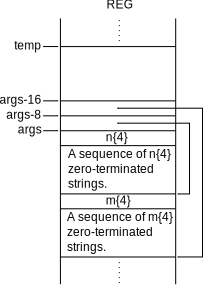
\includegraphics{./fig_prologue_stack_init}
\end{center}
\caption{A layout of stack-initial data received by the Prologue program by reading the stream \#1.}
\label{fig:prologue_stack_init}
\end{figure}

Although a \emph{Prologue program} may be implemented arbitrarily, we recommend
to follow a template of a \emph{Prologue program} for \texttt{x86\_64}
architecture and 64-bit Linux system is depicted in
Tables~\ref{tab:prologue:x86_64_Linux}--\ref{tab:prologue:x86_64_Linux:end}. The
template contains several symbolic constant, listed in
Table~\ref{tab:prologue:x86_64_Linux:constants}, which must be replaced by a
concrete data according to values in the \emph{Descriptor}. We note that the
template reads command line arguments and environment variables from the input
stream \#1 to the \texttt{REG} memory pool as depicted at the
Figure~\ref{fig:prologue_stack_init}. The symbolic constants \textit{temp} and
\textit{args} and defined in Table~\ref{tab:prologue:x86_64_Linux:constants}.
The values \texttt{n\{4\}} and \texttt{m\{4\}} denote counts of command line
arguments and environment variables respectively (i.e. they represent constants
\texttt{argc} and \texttt{envc} mentioned above). The sequence bellow
\texttt{n\{4\}} represents command line arguments and the sequence bellow
\texttt{m\{4\}} environment variables (i.e. pairs of strings). Once the
execution of program is finished the stack is initialised as shown in
Table~\ref{tab:prologue:x86_64_Linux:stack_structure}.

%\redtext{TODO: Add templates also for other platforms.}


\subsection{Reloader}
\label{sec:MAL:reloader}

It is responsible for parsing an assembly file of a \emph{Prologue program} and
filling in the \emph{Descriptor} according to the parsed information. The
\emph{Descriptor} must contain exactly the same information as it would get from
the \emph{Loader} module processing an executable file from which the
\emph{Prologue program} was built by the module \emph{Prologue}.

Note though that in the schema at Figure~\ref{fig:schema_chaining}~(a) there is
used only the ``platform'' data of the \emph{Descriptor}. So, when the
\emph{Reloader} is used in this context, it can optionally be instructed, by
passing a command-line argument `\texttt{--platform-data-only}', to load only
the ``platform'' data to the \emph{Descriptor}.


\subsection{Recogniser}
\label{sec:MAL:recogniser}

It is called from the unit \emph{Analysis}. It accepts a \emph{start address} $
a_0 \in \{0,\ldots,2^{64}-1\} $ into the \texttt{MEM} pool and two
\emph{valuation} functions $ \nu_\mathit{reg}: \{0,\ldots,2^{64}-1\} \rightarrow
\{-1,\ldots,255\} $ and $ \nu_\mathit{mem}: \{0,\ldots,2^{64}-1\} \times \{ r,e
\} \rightarrow \{-3,\ldots,255\} $. Both functions are callback functions. They
allow \emph{Recogniser} to ask \emph{Analysis} for values in contents
\textit{reg} and \textit{mem} of the memory pools \texttt{REG} and \texttt{MEM}
respectively of a considered thread. Namely, $ \nu_\mathit{reg} $ allows for an
access to \textit{reg} and $ \nu_\mathit{mem} $ to \textit{mem} contents of
thread's memory pools. Of course, the \emph{Analysis} may internally represent
the thread and its actual memory state (contents of pools) arbitrarily, in any
(abstract) domain. The \emph{Analysis} thus has to resolve any call $
\nu_\mathit{reg}(a) $ or $ \nu_\mathit{mem}(a,p) $, where $ a \in
\{0,\ldots,2^{64}-1\} $ is any address and $ p \in \{ r,e \} $ is a specifier of
a required access right to the byte at the address $ a $ in the \texttt{MEM}
pool ($ r $ and $ e $ stand for ``read" and ``execute'' rights respectively),
such that it looks up in the current (abstract) state of the thread for a value
of the byte at the address $ a $ in the corresponding memory pool
(i.e.~\textit{reg} in case of $ \nu_\mathit{reg} $ and \textit{mem} in case of $
\nu_\mathit{mem} $). If a single concrete value $ v \in \{0,\ldots,255\} $ is
known at the address $ a $ in the pool and in the case of $ \nu_\mathit{mem} $
the address is also accessible with the right $ p $ (this involves a look up in
the content \textit{sys} of the thread), then $ v $ is returned to the caller
(i.e.~to the \emph{Recogniser}). In all other cases a negative value is
returned, indicating a failure. Namely, for both $ \nu_\mathit{reg} $ and $
\nu_\mathit{mem} $, if a value of the byte is unknown or ambiguous, then the
value $ -1 $ is returned. And in the case of $ \nu_\mathit{mem} $, if the
comparison of $ p $ with access rights of that byte in \textit{sys} leads to
unknown or ambiguous accessibility to the byte, then the value $ -2 $ must be
returned, and if the comparison of $ p $ with access rights of that byte in
\textit{sys} shows inaccessibility of the byte, then the function must return $
-3 $.

The task of the \emph{Recogniser} is to build a Microcode program $ P $ whose
effect is equivalent to the effect of an instruction of the processor
architecture recorded in the \emph{Descriptor} encoded in values of one or more
adjacent bytes in \textit{mem} starting at the address $ a_0 $. In order to
build $ P $ the \emph{Recogniser} may sequentially call the callback functions $
\nu_\mathit{reg} $ and $ \nu_\mathit{mem} $ any number of times (i.e.~another
call to $ \nu_\mathit{reg} $ or $ \nu_\mathit{mem} $ can be issued after a
return value is received from the last call), in any order, and for any
arguments (from domains discussed above). If no call to $ \nu_\mathit{reg} $ and
$ \nu_\mathit{mem} $ returns a negative number, then the \emph{Recogniser} must
return a triple $ (P,\textit{text},\textit{bytes}) $, where $ P $ is a valid
non-empty Microcode program expressing the effect of the instruction encoded in
the values of bytes received from evaluation functions, \textit{text} and
\textit{bytes} are bodies of annotation lines (see
Sections~\ref{sec:microcode:assembly}) with keywords \texttt{ASM.TEXT} and
\texttt{ASM.BYTES} respectively denoting the instruction expressed by $ P $.
Note that \textit{text} must be in the syntax form declared in the annotation
line with the keyword \texttt{ASM.NOTATION} of the \emph{Prologue program}. If $
\nu_\mathit{reg}(a) $ is the first call returning a value $ x < 0 $, then the
\emph{Recogniser} returns a pair $ (1,a) $. And if $ \nu_\mathit{mem}(a,p) $ is
the first call returning a value $ x \in \{-1,-2,-3\} $, then the \emph{Recogniser}
returns a triple $ (2^{-x},a,p) $.
% And if $ \nu_\mathit{mem}(a,p) $ is the first call
%returning a value $ x = -3 $, then the \emph{Recogniser} returns a Microcode
%program $ P $ invoking the processor exception ``memory segmentation fault", see
%the instructions group ``Interrupts'' in Table~\ref{tab:igroup:interrupts}.


The \emph{Recogniser} always first calls $ \nu_\mathit{mem}(a_0,e) $ to get a
value of the first byte of the instruction whose effect should be expressed.
According to the value zero or more calls to valuation functions may follow,
until all information needed for recognition of the native instruction are
collected. It may happen, that values from those calls do not correspond to any
instruction of the considered processor architecture. In this case the \emph{Recogniser} must return a pair $ (16,a_0) $.
% Then the \emph{Recogniser}
%must return a Microcode program $ P $ invoking the processor exception ``not an
%instruction", see the instructions group ``Interrupts'' in
%Table~\ref{tab:igroup:interrupts}.

In Tables~\ref{tab:recogniser:x86_64_examples:begin}--\ref{tab:recogniser:x86_64_examples:end}
we present results from the \emph{Recogniser} for different sequences of bytes
in \texttt{MEM} pool with respect to the \texttt{x86\_64} processor
architecture. The first column defines a number of bytes in the processed
sequence (i.e.~a number of bytes encoding an \texttt{x86\_64} instruction). We
present the sequences itself in the second column in the form of
\texttt{x86\_64} assembly texts in the Intel's syntax. This is due to
readability. And in the third column we show the resulting Microcode program
produced by the \emph{Recogniser}.  In each example, if $ n $ is the number of
bytes, then the \emph{Recogniser} calls $ \nu_\mathit{mem} $ $ n $ times (namely
$ \nu_\mathit{mem}(a_0+0,e), \ldots, \nu_\mathit{mem}(a_0+n-1,e) $, from some
start address $ a_0 $) to get the whole sequence. The \emph{Recogniser} uses a
mapping of \texttt{x86\_64} registers to ranges in \texttt{REG} pool as shown in
Table~\ref{tab:recogniser:x86_64_register_mapping}.

It is sometimes necessary for the \emph{Recogniser} to access also memory outside the range $ [a_0,a_0+n) $ in \texttt{MEM} pool. Consider, for example, ``\texttt{\_exit}" system call on \texttt{x86\_64} architecture:
\begin{center}
\begin{tabular}{l}
\texttt{MOV rax,60~~~~; use the '\_exit' syscall}\\
\texttt{MOV rdi,0~~~~~; error code is 0}\\
\texttt{SYSCALL~~~~~~~; do the syscall}\\
\end{tabular}
\end{center}

The \texttt{SYSCALL} instruction is encoded in two adjacent bytes \texttt{0f}
and \texttt{05}. The \emph{Recogniser} can obtain them in two calls to $
\nu_\mathit{mem} $. Nevertheless, without knowledge of the value of the register
\texttt{rax} it cannot decide, a Microcode program of what system call it should
return the the \emph{Analysis}. The \emph{Recogniser} thus has to further call $
\nu_\mathit{reg} $ eight times to get values of all eight bytes in \texttt{REG}
pool where the register \texttt{rax} is mapped to. From the obtained value 60 it
recognises the ``\_exit" system call and thus it returns the following Microcode
program with two mandatory annotations lines (we express the whole result in
this assembly text):
\begin{center}
\begin{tabular}{l}
\texttt{@ENTRY:}\\
\texttt{~~~~~~~~\#ASM.TEXT: SYSCALL}\\
\texttt{~~~~~~~~\#ASM.BYTES: fh, 5h}\\
\texttt{~~~~STOP}\\
\texttt{~~~~@EXIT}\\
\end{tabular}
\end{center}

\subsubsection{Recogniser's API}
\label{sec:MAL:recogniser:api}

It accepts:
\begin{enumerate}
\item A 64-bit unsigned integer representing the start address $ a_0 $. %
\item A reference to a callback function (e.g.~a pointer to function in
\texttt{C} language) accepting a 64-bit unsigned integer and returning a 16-bit
two's complement integer from the set $ \{-1,\ldots,255\} $. The function must
implement $ \nu_\mathit{reg} $ valuation. %
\item A reference to a callback function (e.g.~a pointer to function in
\texttt{C} language) accepting a 64-bit unsigned integer and an 8-bit unsigned
integer value 1 or 2, representing ``read'' and ``execute'' access rights
respectively, and it returns a 16-bit two's complement integer from the set $
\{-3,\ldots,255\} $. The function must implement $ \nu_\mathit{mem} $ valuation.
%
\end{enumerate}

\noindent
It returns a tuple consisting of 7 elements:
\begin{enumerate}
\item A reference to a resulting Microcode program. If no resulting program is
produced then the reference must be invalid and there must be available a
checking for validity of the reference.  For example, in \texttt{C} language,
the reference can be a pointer and invalid pointer can be \texttt{NULL} pointer.
%
\item A string representing the body of an annotation line \texttt{ASM.TEXT} in
the syntax determined by the annotation \texttt{ASM.NOTATION} in the
\textit{Prologue} program. The string is valid only if the element 1 is a valid
reference. %
\item A string representing the body of an annotation line \texttt{ASM.BYTES}.
The string is valid only if the element 1 is a valid reference. %
\item 8-bit unsigned integer informing about the fact that a call to $
\nu_\mathit{reg} $ or $ \nu_\mathit{mem} $ returned a negative value to the
\textit{Recogniser}. Possible values of this element are:
\begin{center}
\begin{tabular}{cp{5.5cm}}
\textbf{Value} & \textbf{Condition} \\ %
1 & If $ \nu_\mathit{reg} $ returned -1. \\ %
2 & If $ \nu_\mathit{mem} $ returned -1. \\ %
4 & If $ \nu_\mathit{mem} $ returned -2. \\ %
8 & If $ \nu_\mathit{mem} $ returned -3. \\ %
16 & If values received from calls to valuation functions do not represent any
instruction of the considered processor architecture. \\ %
254 & If the \textit{Recogniser} cannot recognise an instruction from concrete
bytes due to its incomplete implementation. \\ %
255 & If the \textit{Recogniser} recognised an instruction from concrete bytes,
but it cannot express it as Microcode program due to its incomplete
implementation.
\end{tabular}
\end{center}
The value matters only if the element 1 is \emph{not} a valid reference to a
resulting program. Note that values 254 and 255 allow \textit{Analyses} to
correctly cooperate with only partially implemented \textit{Recognisers} for
certain platforms. %
\item 64-bit unsigned integer. It is an address passed to a valuation function
returning a negative value. The value matters only if the element 1 is
\emph{not} a valid reference. %
\item 8-bit unsigned integer 1 or 2 representing the access right $ r $ and $ e
$ respectively passed to $ \nu_\mathit{mem} $ returning a negative value. The
value matters only if the element 1 is \emph{not} a valid reference and the
element 4 holds either 2, 4, or 8. %
\item An array of bytes representing the recognised instruction. The array
matters only if the element 1 is a valid reference or if the element 4 holds the
value 255. %
\end{enumerate}

\noindent %
Each valid Microcode program returned from the \textit{Recogniser} must obey the
following conventions:

\begin{itemize}
\item Let $ (u,v) $ be an edge labeled by an instruction of GIK 2+1 or 36+1 writing into the range $ [0,8) $ in the \texttt{REG} pool, and let $ x $ be an exit node from the start component. Then either $ v = x $ or $ (v,x) $ is the only out-edge from $ v $ and it is labeled by instruction of GIK 34+0.
\end{itemize}

\subsection{Encoder}
\label{sec:MAL:encoder}

It provides a translation of a given Microcode program into an equivalent
program of a processor architecture held in the \emph{Descriptor}. The resulting
program is returned in a form of an assembly file of that processor
architecture, ready to be compiled to an executable file for that processor
architecture and the operating system also held in the \emph{Descriptor}.


\clearpage

% % % % % % % % % % % % % % % % % % % % % % % % % % % % % % % % % % % % % % % % %
% % % % % % % % % % % % % % % % % % % % % % % % % % % % % % % % % % % % % % % % %

\begin{table*}[!ht]
\begin{center}
\def\arraystretch{1.5}
\begin{tabular}{rp{12.5cm}}
\textbf{Keyword} & \textbf{Body}
\\

%------------------------------------------------------
\texttt{ASSUMPTION} %
& Any boolean expression (i.e. a formula) over contents \textit{reg},
\textit{mem}, and \textit{sys} of memory pools \texttt{REG}, \texttt{MEM}, and
\texttt{SYS} respectively. The expression must be written in SMT-LIB v2 syntax.
Given unsigned integers $ a, n, n' $ such that $ n,n' \in \{1,2,4,8,10,16\} $
and $ a+n,a+n' \leq 2^{64} $, contents of memory pools can be accessed using
these terms:
\begin{enumerate}
\item  \texttt{(REG} $ a $ $ n $\texttt{)} : It is an integer value stored in
the range $ [a,a+n) $ in \textit{reg}. %

\item  \texttt{(REG (REG} $ a $ \texttt{8)} $ n $\texttt{)} : If $ p $ is an
unsigned integer value stored in the range $ [a,a+8) $ in \textit{reg} and $ p+n
\leq 2^{64}  $, then the term represents an integer value stored in the range $
[p,p+n) $ in \textit{reg}. Otherwise, the meaning of the term is undefined. %

\item  \texttt{(MEM} $ \varphi_{a,8} $ $ n $\texttt{)} : If $ \varphi_{a,8} $ is
either $ a $ or any term of any form 1--4 constructed for values $ a $ and $ n =
8 $ and if it represents (evaluates to) an integer $ p $ such that $ p+n \leq
2^{64}  $ and all addresses in $ [p,p+n) $ are valid according to information
stored in \textit{sys}, then the whole term represents an integer value stored
in the range $ [p,p+n) $ in \textit{mem}. Otherwise, the meaning of the term is
undefined. %

\item  \texttt{(MEM'} $ \varphi_{a,8} $ $ n $\texttt{)} : If $ \varphi_{a,8} $
is either $ a $ or any term of any form 1--4 constructed for values $ a $ and $
n = 8 $ and if it represents (evaluates to) an integer $ p $ such that $ p+n
\leq 2^{64}  $ and all addresses in $ [p,p+n) $ are valid according to
information stored in \textit{sys}, then the whole term represents an integer
value stored in the reversed order in the range $ [p,p+n) $ in \textit{mem}.
Otherwise, the meaning of the term is undefined. %
\end{enumerate}
Moreover, we define the following type-casting terms: TODO!

\textbf{Examples:}\newline
\def\arraystretch{1}
\begin{tabular}[t]{l}
\texttt{\#ASSUMPTION: (= (REG 10h 8) 0)}\\
\texttt{\#ASSUMPTION: (and (= (REG 10h 8) 0) (not (< (REG 20h 8) 0)))}\\
\texttt{\#ASSUMPTION: (= (+ (REG 10h 8) (REG 20h 8)) 1234)}\\
\texttt{\#ASSUMPTION: (= (MEM (MEM' (MEM (REG 10h 8) 8)  8) 4) 1)}
\end{tabular}
\\

%------------------------------------------------------
\texttt{INVARIANT} %
& It has the same structure as \texttt{ASSUMPTION}s.
\\

%------------------------------------------------------
\texttt{OS.TYPE} %
& Names of operating systems: \texttt{LINUX}, \texttt{WINDOWS}, \texttt{MACOS},
\texttt{BSD}. This annotation line can appear at most once in an assembly file.
When present, it should appear between the label line \texttt{@ENTRY} and the
first subsequent instruction or label line.

\textbf{Examples:}\newline
\def\arraystretch{1}
\begin{tabular}[t]{l}
\texttt{\#OS.TYPE: LINUX} \\
\texttt{\#OS.TYPE: WINDOWS} \\
\texttt{\#OS.TYPE: MACOS}
\end{tabular}

\end{tabular}
\end{center}
\caption{Syntax and semantics of annotations lines. (part 1 of 3)}
\label{tab:assembly:annotations}
\end{table*}

%\clearpage

\begin{table*}[!ht]
\begin{center}
\def\arraystretch{1.5}
\begin{tabular}{rp{12.5cm}}
\textbf{Keyword} & \textbf{Body}
\\

%------------------------------------------------------
\texttt{OS.LOADER} %
& Names of operating systems: \texttt{ld\_linux\_x86\_64\_so\_2},
\texttt{ld\_linux\_x86\_32\_so\_2}, \texttt{ld\_linux\_uClibc\_so\_0},
\texttt{WINDOWS}, \texttt{DARWIN}. This annotation line can appear at most once
in an assembly file. When present, it should appear between the label line
\texttt{@ENTRY} and the first subsequent instruction or label line.

\textbf{Examples:}\newline
\def\arraystretch{1}
\begin{tabular}[t]{l}
\texttt{\#OS.LOADER: ld\_linux\_x86\_64\_so\_2} \\
\texttt{\#OS.LOADER: WINDOWS} \\
\texttt{\#OS.LOADER: DARWIN}
\end{tabular}
\\

%------------------------------------------------------
\texttt{OS.SUBSYSTEM} %
& Names of operating systems: \texttt{NATIVE}, \texttt{GUI}, \texttt{CUI},
\texttt{POSIX\_CUI}, \texttt{WINDOWS\_CE}, \texttt{EFI}. This annotation line
can appear at most once in an assembly file. When present, it should appear
between the label line \texttt{@ENTRY} and the first subsequent instruction or
label line.

\textbf{Examples:}\newline
\def\arraystretch{1}
\begin{tabular}[t]{l}
\texttt{\#OS.SUBSYSTEM: NATIVE} \\
\texttt{\#OS.SUBSYSTEM: GUI} \\
\texttt{\#OS.SUBSYSTEM: CUI}
\end{tabular}
\\

%------------------------------------------------------
\texttt{CPU.ARCHITECTURE} %
& Names of processor architectures: \texttt{X86-32}, \texttt{X86-64},
\texttt{ARM}, \texttt{ARM64}, \texttt{MIPS}, \texttt{SPARC}, \texttt{POWERPC}.
This annotation line can appear at most once in an assembly file. When present,
it should appear between the label line \texttt{@ENTRY} and the first subsequent
instruction or label line.

\textbf{Examples:}\newline
\def\arraystretch{1}
\begin{tabular}[t]{l}
\texttt{\#CPU.ARCHITECTURE: X86-64}\\
\texttt{\#CPU.ARCHITECTURE: MIPS}\\
\texttt{\#CPU.ARCHITECTURE: SPARC}
\end{tabular}
\\

%------------------------------------------------------
\texttt{CPU.IP} %
& A current value of CPU's \emph{Instruction Pointer} (IP) register. The value
is a 64-bit hexadecimal unsigned integer suffixed by `h'. It represents an
absolute address.

\textbf{Examples:}\newline
\def\arraystretch{1}
\begin{tabular}[t]{l}
\texttt{\#CPU.IP: 4000b0h}
\end{tabular}
\\

%------------------------------------------------------
\texttt{ASM.NOTATION} %
& Any of the following string constant identifying what assembler notation is
used (there can be several for the same processor architecture from different
vendors): \texttt{INTEL}, \texttt{AT\&T}. This annotation line can appear at
most once in an assembly file. When present, it should appear between the label
line \texttt{@ENTRY} and the first subsequent instruction or label line.

\textbf{Examples:}\newline
\def\arraystretch{1}
\begin{tabular}[t]{l}
\texttt{\#ASM.NOTATION: INTEL}\\
\texttt{\#ASM.NOTATION: AT\&T}
\end{tabular}

\end{tabular}
\end{center}
\caption{Syntax and semantics of annotations lines. (part 2 of 3)}
\end{table*}


%\clearpage

\begin{table*}[!ht]
\begin{center}
\def\arraystretch{1.5}
\begin{tabular}{rp{12.5cm}}
\textbf{Keyword} & \textbf{Body}
\\

%------------------------------------------------------
\texttt{ASM.TEXT} %
& A textual (assembly) representation of an instruction of the \texttt{CPU.ARCHITECTURE} in the \texttt{ASM.NOTATION}.

\textbf{Examples:}\newline
\def\arraystretch{1}
\begin{tabular}[t]{l}
\texttt{\#ASM.TEXT: MOV eax,ffh} \\
\texttt{\#ASM.TEXT: MOVL \$0xff,\%eax} \\
\end{tabular}
\\


%------------------------------------------------------
\texttt{ASM.BYTES} %
& A sequence of comma-separated unsigned integers representing values of
adjacent bytes in the memory where some processor instruction is encoded. Either
all the numbers are decimal or hexadecimal. In the later case they all must be
lower-case and terminated by 'h'. %

\textbf{Examples:}\newline
\def\arraystretch{1}
\begin{tabular}[t]{l}
\texttt{\#ASM.BYTES: 123,11,58,64}\\
\texttt{\#ASM.BYTES: 7bh, bh, 3ah, 40h}\\
\end{tabular}
\\

%------------------------------------------------------
\texttt{PROGRAM.NAME} %
& A name of the Microcode program. This annotation can only by attached to the
entry node of the start component. %
\\

%------------------------------------------------------
\texttt{COMPONENT.NAME} %
& A name of a component of the Microcode program. This annotation can only by
attached to the entry node of a component. %
\\

%%------------------------------------------------------
%\texttt{} %
%& %
%
%\textbf{Examples:}\newline
%\def\arraystretch{1}
%\begin{tabular}[t]{l}
%\texttt{\#:}\\
%\end{tabular}
%\\

\end{tabular}
\end{center}
\caption{Syntax and semantics of annotations lines. (part 3 of 3)}
\label{tab:assembly:annotations:end}
\end{table*}

\clearpage

% % % % % % % % % % % % % % % % % % % % % % % % % % % % % % % % % % % % % % % % %
% % % % % % % % % % % % % % % % % % % % % % % % % % % % % % % % % % % % % % % % %

\begin{table*}[!h]
\begin{center}
\def\arraystretch{1}
\begin{tabular}{rp{10cm}}
\textbf{Symbol} & \textbf{Description} \\

$ p $ %
& A number of code sections in the executable file and dependent shared
libraries, if any. %
\\

$ q $ %
& A number of data sections in the executable file and dependent shared
libraries, if any. %
\\

$ r $ %
& A number of adjacent memory blocks representing the whole memory reserved for
the stack. %
\\

\textit{code\_begin}$ _i $ %
& A start address of the $ i $-th code section, $ i = 1,\ldots,p $. %
\\

\textit{code\_size}$ _i $ %
& A number of bytes of the $ i $-th code section, $ i = 1,\ldots,p $. %
\\

\textit{code\_rights}$ _i $ %
& An access rights to the $ i $-th code section, $ i = 1,\ldots,p $. %
\\

\textit{code\_values}$ _i $ %
& A comma-separated list of \textit{code\_size}$ _i $ numbers representing
values of all bytes the $ i $-th code section, $ i = 1,\ldots,p $. %
\\

\textit{data\_begin}$ _i $ %
& A start address of the $ i $-th data section, $ i = 1,\ldots,q $. %
\\

\textit{data\_size}$ _i $ %
& A number of bytes of the $ i $-th data section, $ i = 1,\ldots,q $. %
\\

\textit{data\_rights}$ _i $ %
& An access rights to the $ i $-th data section, $ i = 1,\ldots,q $. %
\\

\textit{data\_values}$ _i $ %
& A comma-separated list of \textit{data\_size}$ _i $ numbers representing
values of all bytes the $ i $-th data section, $ i = 1,\ldots,p $. %
\\

\textit{stack\_begin}$ _i $ %
& A start address of the $ i $-th block of memory reserved for the stack, $ i =
1,\ldots,r $. %
\\

\textit{stack\_size}$ _i $ %
& A number of bytes of $ i $-th block of memory reserved for the stack, $ i =
1,\ldots,r $. %
\\

\textit{stack\_right}$ _i $ %
& An access rights of $ i $-th block of the memory reserved for the stack, $ i =
1,\ldots,r $. %
\\

\textit{atexit\_routine\_entry} %
& An address of the entry point to a system-defined routine to be pushed into
the ``atexit" stack. %
\\

\textit{executable\_entry\_point} %
& The entry point address of the executable file. %
\\

\textit{temp} %
& An address into the \textit{REG} pool where start temporaries.
%
\\

\textit{args} %
& A start address into the \textit{REG} pool where program arguments (\texttt{argc} and \texttt{argv}) are stored before they are moved to the stack. $ \mathit{args} \geq
\mathit{temp} + 60 $. %
\\

\textit{rsp} %
& An start address into \texttt{REG} pool where is mapped the register \texttt{rsp}.
%
\\

\textit{rdx} %
& An start address into \texttt{REG} pool where is mapped the register \texttt{rdx}.
%
\\

\end{tabular}
\end{center}
\caption{A description of symbolic constant used in the template \emph{Prologue
program} in
Tables~\ref{tab:prologue:x86_64_Linux}--\ref{tab:prologue:x86_64_Linux:end}.} %
\label{tab:prologue:x86_64_Linux:constants}
\end{table*}

\clearpage

% % % % % % % % % % % % % % % % % % % % % % % % % % % % % % % % % % % % % % % % %
% % % % % % % % % % % % % % % % % % % % % % % % % % % % % % % % % % % % % % % % %

\begin{table*}[!h]
\begin{center}
\def\arraystretch{1}
\begin{tabular}{l||p{3.5cm}|p{3.5cm}|p{7cm}}
\textbf{\#} &
\textbf{Start address} &
\textbf{Size in bytes} &
\textbf{Content} \\
\hline\hline

0 %
& \textit{stack\_begin}$ _0 $ %
& \texttt{REG[}\textit{rsp}\texttt{]\{8\}}$ - $ \textit{stack\_begin}$ _0 $ %
& Undefined. The memory bellow \texttt{rsp} is reserved for frames of future
function calls. The stack grows from higher to lower addresses, i.e.~from
\texttt{REG[}\textit{rsp}\texttt{]\{8\}} down to \textit{stack\_begin}$ _0 $. %
\\ \hline

1 %
& \texttt{REG[}\textit{rsp}\texttt{]\{8\}} %
& 8 %
& A number of program arguments, i.e.~\texttt{argc} in C language. Observe that
the value \texttt{REG[}\textit{rsp}\texttt{]\{8\}} of the stack pointer register
is the address of this number. %
\\ \hline

2 %
& %\texttt{REG[}\textit{rsp}\texttt{]\{8\}}$ + 8$ %
& 8$ \cdot $\texttt{REG[REG[}\textit{rsp}\texttt{]\{8\}]\{8\}} %
& An array of pointers to zero-terminated strings representing program
arguments, i.e.~\texttt{argv} in C language. The strings are stored in \#4. The
number of pointers (and strings) is stored in the block \#1.%
\\ \hline

3 %
&
& 8 %
& \texttt{0\{8\}}
\\ \hline

4 %
& 
& \textit{varies} %
& A list of 64-bit addresses of zero-terminated strings representing environment
variables. The pointed strings are stored in block \#5. \\ \hline

5 %
&
& 8 %
& \texttt{0\{8\}}
\\ \hline

6 %
& %
& 0 %
& A vector of pairs (auxiliary entries) consisting of two 8-bytes long elements
(``type" and ``data", where ``data" can actually be a pointer to data/routine of
any length stored in \#5). The length of this block is zero, because a
\textit{Prologue program} does not generates these data. \\ \hline

7 %
&
& 8 %
& \texttt{0\{8\}}
\\ \hline

8 %
& %
& \textit{varies} %
& A minimal number of bytes of unspecified values ensuring 16-bytes alignment of
\texttt{REG[}\textit{rsp}\texttt{]\{8\}}. A \textit{Prologue program} should
choose the value 0 for these bytes. \\ \hline

9 %
& %
& \textit{varies} %
& A sequence of \texttt{REG[REG[}\textit{rsp}\texttt{]\{8\}]\{8\}}
zero-terminated strings pointed to by elements of the array in \#2.%
\\ \hline

10 %
& %
& \textit{varies} %
& Strings of environment variables pointed to by elements of the list in \#4.%
\\ \hline

11 %
& %
& 0 %
& A data/routines pointed to by auxiliary entries of the vector in \#6 and
possibly other system-dependent information in unspecified format. The length of
this block is zero, because a \textit{Prologue program} does not generates these
data. %
\\ \hline

\end{tabular}
\end{center}
\caption{A content of stack as it is constructed by the template \emph{Prologue
program} in
Tables~\ref{tab:prologue:x86_64_Linux}--\ref{tab:prologue:x86_64_Linux:end}.} %
\label{tab:prologue:x86_64_Linux:stack_structure}
\end{table*}

\clearpage


% % % % % % % % % % % % % % % % % % % % % % % % % % % % % % % % % % % % % % % % %
% % % % % % % % % % % % % % % % % % % % % % % % % % % % % % % % % % % % % % % % %

\begin{table*}[!h]
\begin{center}
\def\arraystretch{1}
\begin{tabular}{l}

%------------------------------------------------------------------
\texttt{@PROLOGUE\_init\_code\_and\_data\_sections:}\\ %

\texttt{~~~~* }\textit{code\_begin}$ _1 $\texttt{\{8\} :=
[~}\textit{code\_values}$ _1 $\texttt{~]\{}\textit{code\_size}$ _1
$\texttt{\}}\\ %
\texttt{~~~~...}\\ %
\texttt{~~~~* }\textit{code\_begin}$ _p $\texttt{\{8\} :=
[~}\textit{code\_values}$ _p $\texttt{~]\{}\textit{code\_size}$ _p
$\texttt{\}}\\ %

\texttt{~~~~* }\textit{data\_begin}$ _1 $\texttt{\{8\} :=
[~}\textit{data\_values}$ _1 $\texttt{~]\{}\textit{data\_size}$ _1
$\texttt{\}}\\ %
\texttt{~~~~...}\\ %
\texttt{~~~~* }\textit{data\_begin}$ _q $\texttt{\{8\} :=
[~}\textit{data\_values}$ _q $\texttt{~]\{}\textit{data\_size}$ _q
$\texttt{\}}\\ %

\texttt{~~~~@EXIT}\\ %
\\ \\

%%------------------------------------------------------------------
%\texttt{@PROLOGUE\_init\_stack\_aeinfo:}\\ %
%
%\texttt{~~~~* }\textit{aeinfo\_begin}\texttt{\{8\} :=
%[~}\textit{aeinfo\_values}\texttt{~]\{}\textit{aeinfo\_size}\texttt{\}}\\ %
%\texttt{~~~~* }(\textit{aeinfo\_begin}$ - $\textit{exename\_size}$ - 1$)\texttt{\{8\} :=
%[~}\textit{exename}\texttt{~]\{}\textit{exename\_size$ +1 $}\texttt{\}}\\ %
%\texttt{~~~~@EXIT}\\ %
%\\ \\
%
%%------------------------------------------------------------------
%\texttt{@PROLOGUE\_init\_stack\_aeptrs:}\\ %
%
%\texttt{~~~~*} \texttt{REG[}\textit{temp}\texttt{]\{8\} :=
%[~}\textit{aeptrs\_values}\texttt{~]\{}\textit{aeptrs\_size}\texttt{\}}\\ %
%\texttt{~~~~@EXIT}\\ %
%\\ \\


%------------------------------------------------------------------
\texttt{@ENTRY:}\\ %

\texttt{~~~~~~~~\#PROGRAM.NAME: Prologue}\\ %
\texttt{~~~~~~~~\#CPU.ARCHITECTURE: X86-64}\\ %
\texttt{~~~~~~~~\#OS.TYPE: LINUX}\\ %
\texttt{~~~~~~~~\#OS.LOADER: ld\_linux\_x86\_64\_so\_2}\\ %
\texttt{~~~~~~~~\#ASM.NOTATION: INTEL}\\ %

\texttt{~~~~REG[}\textit{temp}\texttt{]\{8\} := MEM STATIC
}\textit{code\_rights}$ _1 $\texttt{\{1\}, }\textit{code\_size}$ _1 $\texttt{\{8\},}
\textit{code\_begin}$ _1 $\texttt{\{8\}}\\ %
\texttt{~~~~...}\\ %
\texttt{~~~~REG[}\textit{temp}\texttt{]\{8\} := MEM STATIC
}\textit{code\_rights}$ _p $\texttt{\{1\}, }\textit{code\_size}$ _p $\texttt{\{8\},}
\textit{code\_begin}$ _p $\texttt{\{8\}}\\ %

\texttt{~~~~REG[}\textit{temp}\texttt{]\{8\} := MEM STATIC
}\textit{data\_rights}$ _1 $\texttt{\{1\}, }\textit{data\_size}$ _1 $\texttt{\{8\},}
\textit{data\_begin}$ _1 $\texttt{\{8\}}\\ %
\texttt{~~~~...}\\ %
\texttt{~~~~REG[}\textit{temp}\texttt{]\{8\} := MEM STATIC
}\textit{data\_rights}$ _q $\texttt{\{1\}, }\textit{data\_size}$ _q $\texttt{\{8\},}
\textit{data\_begin}$ _q $\texttt{\{8\}}\\ %

\texttt{~~~~REG[}\textit{temp}\texttt{]\{8\} := MEM STATIC
}\textit{stack\_rights}$ _1 $\texttt{\{1\}, }\textit{stack\_size}$ _1
$\texttt{\{8\},} \textit{stack\_begin}$ _1 $\texttt{\{8\}}\\ %
\texttt{~~~~...}\\ %
\texttt{~~~~REG[}\textit{temp}\texttt{]\{8\} := MEM STATIC
}\textit{stack\_rights}$ _r $\texttt{\{1\}, }\textit{stack\_size}$ _r
$\texttt{\{8\},} \textit{stack\_begin}$ _r $\texttt{\{8\}}\\ %

\texttt{~~~~REG[}\textit{temp}\texttt{]\{8\} := STREAM OPEN 1\{1\}, 1\{8\}}\\ %
\texttt{~~~~REG[}\textit{temp}\texttt{]\{8\} := STREAM OPEN 2\{1\}, 2\{8\}}\\ %
\texttt{~~~~REG[}\textit{temp}\texttt{]\{8\} := STREAM OPEN 2\{1\}, 3\{8\}}\\ %
\texttt{~~~~REG[}\textit{temp}\texttt{]\{8\} := STREAM OPEN 2\{1\}, 4\{8\}}\\ %

\texttt{~~~~CALL PROLOGUE\_init\_code\_and\_data\_sections}\\ %
\texttt{~~~~CALL PROLOGUE\_init\_stack}\\ %
\texttt{~~~~REG[}\textit{rdx}\texttt{]\{8\} :=
}\textit{atexit\_routine\_entry}\texttt{\{8\}}\\ %
\texttt{~~~~REG[0]\{8\} := }\textit{executable\_entry\_point}\texttt{\{8\}}\\ %
\texttt{~~~~@EXIT}\\ %
\\ \\


%------------------------------------------------------------------
\texttt{@PROLOGUE\_read\_count:}\\ %
\texttt{~~~~REG[}\textit{temp}$ +8 $\texttt{]\{1\} := STREAM READ 1\{8\}}\\ %
\texttt{~~~~REG[}\textit{temp}$ +9 $\texttt{]\{1\} := STREAM READ 1\{8\}}\\ %
\texttt{~~~~REG[}\textit{temp}$ +10 $\texttt{]\{1\} := STREAM READ 1\{8\}}\\ %
\texttt{~~~~REG[}\textit{temp}$ +11 $\texttt{]\{1\} := STREAM READ 1\{8\}}\\ %
\texttt{~~~~REG[REG[}\textit{temp}\texttt{]\{8\}]\{4\} := REG[}\textit{temp}$ +8
$\texttt{]\{4\}}\\ %
\texttt{~~~~@EXIT}\\ %

\end{tabular}
\end{center}
\caption{A template \emph{Prologue program} for ELF files on 64-bit Linux and
x86-64 CPU. (part 1 of 4)} %
\label{tab:prologue:x86_64_Linux}
\end{table*}

\begin{table*}[!h]
\vspace{-0.5cm}
\begin{center}
\def\arraystretch{1}
\begin{tabular}{l}

%------------------------------------------------------------------
\texttt{@PROLOGUE\_read\_strings:}\\ %
\texttt{~~~~REG[}\textit{temp}$ +8 $\texttt{]\{4\} := 0\{4\}}\\ %
\texttt{@PROLOGUE\_read\_next\_string:}\\ %
\texttt{~~~~REG[}\textit{temp}$ +16 $\texttt{]\{4\} := REG[}\textit{temp}$ +8
$\texttt{]\{4\} XOR\{4\} REG[}\textit{temp}$ +12 $\texttt{]\{4\}}\\ %
\texttt{~~~~@PROLOGUE\_read\_string REG[}\textit{temp}$ +16 $\texttt{]\{4\}
!=\{4\} 0\{4\} @EXIT}\\ %
\texttt{@PROLOGUE\_read\_string:}\\ %
\texttt{~~~~REG[}\textit{temp}$ +16 $\texttt{]\{1\} := STREAM READ 1\{8\}}\\ %
\texttt{~~~~REG[REG[}\textit{temp}\texttt{]\{8\}]\{1\} := REG[}\textit{temp}$
+16 $\texttt{]\{1\}}\\ %
\texttt{~~~~REG[}\textit{temp}\texttt{]\{8\} := REG[}\textit{temp}\texttt{]\{8\}
+\{8\} 1\{8\}}\\ %
\texttt{~~~~@PROLOGUE\_read\_string REG[}\textit{temp}$ +16 $\texttt{]\{1\}
!=\{1\} 0\{1\} @PROLOGUE\_string\_end}\\ %
\texttt{@PROLOGUE\_string\_end:}\\ %
\texttt{~~~~REG[}\textit{temp}$ +8 $\texttt{]\{4\} := REG[}\textit{temp}$ +8
$\texttt{]\{4\} +\{4\} 1\{4\}}\\ %
\texttt{~~~~@PROLOGUE\_read\_next\_string}\\ %
\\ \\


%------------------------------------------------------------------
\texttt{@PROLOGUE\_read\_input\_data:}\\ %
\texttt{~~~~REG[}\textit{temp}\texttt{]\{8\} := }\textit{args}\texttt{\{8\}}\\ %
\texttt{~~~~CALL PROLOGUE\_read\_count}\\ %
\texttt{~~~~REG[}\textit{temp}$ +12 $\texttt{]\{4\} :=
REG[REG[}\textit{temp}\texttt{]\{8\}]\{4\}}\\ %
\texttt{~~~~REG[}\textit{temp}\texttt{]\{8\} := REG[}\textit{temp}\texttt{]\{8\}
+ 4\{8\}}\\ %
\texttt{~~~~CALL PROLOGUE\_read\_strings}\\ %
\texttt{~~~~REG[}\textit{args}$ -8 $\texttt{]\{8\} :=
REG[}\textit{temp}\texttt{]\{8\}}\\ %
\texttt{~~~~CALL PROLOGUE\_read\_count}\\ %
\texttt{~~~~REG[}\textit{temp}$ +12 $\texttt{]\{4\} :=
REG[REG[}\textit{temp}\texttt{]\{8\}]\{4\}}\\ %
\texttt{~~~~REG[}\textit{temp}$ +12 $\texttt{]\{4\} := REG[}\textit{temp}$ +12
$\texttt{]\{4\} *\{4\} 2\{4\}}\\ %
\texttt{~~~~REG[}\textit{temp}\texttt{]\{8\} := REG[}\textit{temp}\texttt{]\{8\}
+ 4\{8\}}\\ %
\texttt{~~~~CALL PROLOGUE\_read\_strings}\\ %
\texttt{~~~~REG[}\textit{args}$ -16 $\texttt{]\{8\} :=
REG[}\textit{temp}\texttt{]\{8\}}\\ %
\texttt{~~~~@EXIT}\\ %
\\ \\


%------------------------------------------------------------------
\texttt{@PROLOGUE\_compute\_stack\_pointers:}\\ %
\texttt{~~~~REG[}\textit{temp}\texttt{]\{8\} := !\{8\} REG[}\textit{args}$ -16
$\texttt{]\{8\}}\\ %
\texttt{~~~~REG[}\textit{args}$ -24 $\texttt{]\{8\} :=
REG[}\textit{temp}\texttt{]\{8\} +\{8\} } $ ( $\textit{stack\_end}$ +
$\textit{args}$ + 5) $\texttt{\{8\}}\\ %
\texttt{~~~~REG[}\textit{temp}\texttt{]\{8\} := \#z
REG[}\textit{args}\texttt{]\{4\}}\\ %
\texttt{~~~~REG[}\textit{temp}$ +8 $\texttt{]\{4\} := REG[REG[}\textit{args}$ -8
$\texttt{]\{8\}]\{4\}}\\ %
\texttt{~~~~REG[}\textit{temp}$ +8 $\texttt{]\{8\} := \#z REG[}\textit{temp}$ +8
$\texttt{]\{4\}}\\ %
\texttt{~~~~REG[}\textit{temp}\texttt{]\{8\} := REG[}\textit{temp}\texttt{]\{8\}
+\{8\} REG[}\textit{temp}$ +8 $\texttt{]\{8\}}\\ %
\texttt{~~~~REG[}\textit{temp}\texttt{]\{8\} := REG[}\textit{temp}\texttt{]\{8\}
*\{8\} 8\{8\}}\\ %
\texttt{~~~~REG[}\textit{temp}\texttt{]\{8\} := REG[}\textit{temp}\texttt{]\{8\}
+\{8\} 32\{8\}}\\ %
\texttt{~~~~REG[}\textit{temp}\texttt{]\{8\} := !\{8\}
REG[}\textit{temp}\texttt{]\{8\}}\\ %
\texttt{~~~~REG[}\textit{temp}\texttt{]\{8\} := REG[}\textit{temp}\texttt{]\{8\}
+\{8\} REG[}\textit{args}$ -24 $\texttt{]\{8\}}\\ %
\texttt{~~~~REG[}\textit{rsp}\texttt{]\{8\} := REG[}\textit{temp}\texttt{]\{8\}
+\{8\} 1\{8\}}\\ %
\texttt{~~~~REG[}\textit{rsp}$ +7 $\texttt{]\{1\} := REG[}\textit{rsp}$ +7
$\texttt{]\{1\} \&\{1\} f0h\{1\}}\\ %
\texttt{~~~~@EXIT}\\ %

\end{tabular}
\end{center}
\caption{A template \emph{Prologue program} for ELF files on 64-bit Linux and
x86-64 CPU. (part 2 of 4)} %
\end{table*}

\begin{table*}[!h]
\begin{center}
\def\arraystretch{1}
\begin{tabular}{l}


\texttt{@PROLOGUE\_copy\_string\_to\_stack:}\\ %
\texttt{~~~~REG[}\textit{temp}$ +32 $\texttt{]\{1\} := REG[REG[}\textit{temp}$
+16 $\texttt{]\{8\}]\{1\}}\\ %
\texttt{~~~~* REG[}\textit{temp}$ +8 $\texttt{]\{8\} := REG[}\textit{temp}$ +32
$\texttt{]\{1\} }\\ %
\texttt{~~~~REG[}\textit{temp}$ +8 $\texttt{]\{8\} := REG[}\textit{temp}$ +8
$\texttt{]\{8\} +\{8\} 1\{8\}}\\ %
\texttt{~~~~REG[}\textit{temp}$ +16 $\texttt{]\{8\} := REG[}\textit{temp}$ +16
$\texttt{]\{8\} +\{8\} 1\{8\}}\\ %
\texttt{~~~~@PROLOGUE\_copy\_string\_to\_stack REG[}\textit{temp}$ +32 $\texttt{]\{1\}
!=\{1\} 0\{1\} @EXIT}\\ %
\\ \\


%------------------------------------------------------------------
\texttt{@PROLOGUE\_copy\_params\_to\_stack:}\\ %
\texttt{~~~~REG[}\textit{temp}$ +24 $\texttt{]\{8\} := \#z
REG[}\textit{args}\texttt{]\{4\} }\\ %
\texttt{~~~~*' REG[}\textit{rsp}\texttt{]\{8\} := REG[}\textit{temp}$ +24
$\texttt{]\{8\} }\\ %
\texttt{~~~~REG[}\textit{temp}$ +24 $\texttt{]\{4\} := 0\{4\}}\\ %
\texttt{@PROLOGUE\_copy\_next\_param:}\\ %
\texttt{~~~~REG[}\textit{temp}$ +28 $\texttt{]\{4\} := REG[}\textit{temp}$ +24
$\texttt{]\{4\} XOR\{4\} REG[}\textit{args}\texttt{]\{4\}}\\ %
\texttt{~~~~@PROLOGUE\_copy\_param REG[}\textit{temp}$ +28 $\texttt{]\{4\}
!=\{4\} 0\{4\} @EXIT}\\ %
\texttt{@PROLOGUE\_copy\_param:}\\ %
\texttt{~~~~*' REG[}\textit{temp}\texttt{]\{8\} := REG[}\textit{temp}$ +8
$\texttt{]\{8\} }\\ %
\texttt{~~~~REG[}\textit{temp}\texttt{]\{8\} := REG[}\textit{temp}\texttt{]\{8\}
+\{8\} 8\{8\}}\\ %
\texttt{~~~~CALL PROLOGUE\_copy\_string\_to\_stack}\\ %
%\texttt{@PROLOGUE\_copy\_param:}\\ %
%\texttt{~~~~REG[}\textit{temp}$ +28 $\texttt{]\{1\} := REG[REG[}\textit{temp}$
%+16 $\texttt{]\{8\}]\{1\}}\\ %
%\texttt{~~~~* REG[}\textit{temp}$ +8 $\texttt{]\{1\} := REG[}\textit{temp}$ +28
%$\texttt{]\{1\} }\\ %
%\texttt{~~~~REG[}\textit{temp}$ +8 $\texttt{]\{8\} := REG[}\textit{temp}$ +8
%$\texttt{]\{8\} +\{8\} 1\{8\}}\\ %
%\texttt{~~~~REG[}\textit{temp}$ +16 $\texttt{]\{8\} := REG[}\textit{temp}$ +16
%$\texttt{]\{8\} +\{8\} 1\{8\}}\\ %
%\texttt{~~~~@PROLOGUE\_copy\_param REG[}\textit{temp}$ +28 $\texttt{]\{4\}
%!=\{4\} 0\{4\} @PROLOGUE\_param\_end}\\ %
%\texttt{@PROLOGUE\_param\_end:}\\ %
\texttt{~~~~REG[}\textit{temp}$ +24 $\texttt{]\{4\} := REG[}\textit{temp}$ +24
$\texttt{]\{4\} +\{4\} 1\{4\}}\\ %
\texttt{~~~~@PROLOGUE\_copy\_next\_param}\\ %
\\ \\


%------------------------------------------------------------------
\texttt{@PROLOGUE\_copy\_env\_to\_stack:}\\ %
\texttt{~~~~REG[}\textit{temp}$ +24 $\texttt{]\{4\} := 0\{4\}}\\ %
\texttt{~~~~REG[}\textit{temp}$ +28 $\texttt{]\{4\} := REG[REG[}\textit{temp}$
+16 $\texttt{]\{8\}]\{4\}}\\ %
\texttt{~~~~REG[}\textit{temp}$ +16 $\texttt{]\{8\} := REG[}\textit{temp}$ +16
$\texttt{]\{8\} +\{8\} 4\{8\}}\\ %
\texttt{@PROLOGUE\_copy\_next\_var:}\\ %
\texttt{~~~~REG[}\textit{temp}$ +32 $\texttt{]\{4\} := REG[}\textit{temp}$ +24
$\texttt{]\{4\} XOR\{4\} REG[}\textit{temp}$ +28 $\texttt{]\{4\}}\\ %
\texttt{~~~~@PROLOGUE\_copy\_var REG[}\textit{temp}$ +32 $\texttt{]\{4\} !=\{4\}
0\{4\} @EXIT}\\ %
\texttt{@PROLOGUE\_copy\_var:}\\ %
\texttt{~~~~*' REG[}\textit{temp}\texttt{]\{8\} := REG[}\textit{temp}$ +8
$\texttt{]\{8\} }\\ %
\texttt{~~~~REG[}\textit{temp}\texttt{]\{8\} := REG[}\textit{temp}\texttt{]\{8\}
+\{8\} 8\{8\}}\\ %
\texttt{~~~~CALL PROLOGUE\_copy\_string\_to\_stack}\\ %
\texttt{~~~~REG[}\textit{temp}$ +32 $\texttt{]\{8\} := REG[}\textit{temp}$ +8
$\texttt{]\{8\} +\{8\} ffffffffffffffffh\{8\}}\\ %
\texttt{~~~~* REG[}\textit{temp}$ +32 $\texttt{]\{1\} := 3dh\{1\} }\\ %
%\texttt{~~~~REG[}\textit{temp}$ +8 $\texttt{]\{8\} := REG[}\textit{temp}$ +8
%$\texttt{]\{8\} +\{8\} 1h\{8\}}\\ %
\texttt{~~~~CALL PROLOGUE\_copy\_string\_to\_stack}\\ %
\texttt{~~~~REG[}\textit{temp}$ +24 $\texttt{]\{4\} := REG[}\textit{temp}$ +24
$\texttt{]\{4\} +\{4\} 1\{4\}}\\ %
\texttt{~~~~@PROLOGUE\_copy\_next\_var}\\ %


\end{tabular}
\end{center}
\caption{A template \emph{Prologue program} for ELF files on 64-bit Linux and
x86-64 CPU. (part 3 of 4)} %
\end{table*}

\begin{table*}[!h]
\begin{center}
\def\arraystretch{1}
\begin{tabular}{l}



%------------------------------------------------------------------
\texttt{@PROLOGUE\_set\_alignment\_zeros:}\\ %
\texttt{~~~~REG[}\textit{temp}$ +16 $\texttt{]\{8\} := REG[}\textit{temp}\texttt{]\{8\} XOR\{8\} REG[}\textit{args}$ -24 $\texttt{]\{8\}}\\ %
\texttt{~~~~@PROLOGUE\_clear\_byte REG[}\textit{temp}$ +16 $\texttt{]\{8\}
!=\{8\} 0\{8\} @EXIT}\\ %
\texttt{@PROLOGUE\_clear\_byte:}\\ %
\texttt{~~~~* REG[}\textit{temp}\texttt{]\{1\} := 0\{1\} }\\ %
\texttt{~~~~REG[}\textit{temp}\texttt{]\{8\} := REG[}\textit{temp}\texttt{]\{8\}
+\{8\} 1\{8\}}\\ %
\texttt{~~~~@PROLOGUE\_set\_alignment\_zeros}\\ %
\\ \\

%------------------------------------------------------------------
\texttt{@PROLOGUE\_havoc\_used\_temporaries:}\\ %
\texttt{~~~~REG[}\textit{temp}\texttt{]\{8\} := }\textit{args}\texttt{\{8\}}\\ %
\texttt{@PROLOGUE\_havoc\_input:}\\ %
\texttt{~~~~REG[}\textit{temp}$ +8 $\texttt{]\{8\} :=
REG[}\textit{temp}\texttt{]\{8\} XOR\{8\} REG[}\textit{args}$ -16
$\texttt{]\{8\}}\\ %
\texttt{~~~~@PROLOGUE\_havoc\_byte REG[}\textit{temp}$ +8 $\texttt{]\{8\}
!=\{8\} 0\{8\} @PROLOGUE\_havoc\_remaining}\\ %
\texttt{@PROLOGUE\_havoc\_byte:}\\ %
\texttt{~~~~REG[REG[}\textit{temp}\texttt{]\{8\}]\{1\}:= HAVOC}\\ %
\texttt{~~~~REG[}\textit{temp}\texttt{]\{8\} := REG[}\textit{temp}\texttt{]\{8\}
+\{8\} 1\{8\}}\\ %
\texttt{~~~~@PROLOGUE\_havoc\_input}\\ %
\texttt{@PROLOGUE\_havoc\_remaining:}\\ %
\texttt{~~~~REG[}\textit{temp}\texttt{]\{}\textit{args}$ -
$\textit{temp}\texttt{\} := HAVOC}\\ %
\texttt{~~~~@EXIT}\\ %
\\ \\


%------------------------------------------------------------------
\texttt{@PROLOGUE\_init\_stack:}\\ %
\texttt{~~~~CALL PROLOGUE\_read\_input\_data}\\ %
\texttt{~~~~CALL PROLOGUE\_compute\_stack\_pointers}\\ %
\texttt{~~~~REG[}\textit{temp}\texttt{]\{8\} := REG[}\textit{rsp}\texttt{]\{8\}
+\{8\} 8\{8\}}\\ %
\texttt{~~~~REG[}\textit{temp}$ +8 $\texttt{]\{8\} := REG[}\textit{args}$ -24
$\texttt{]\{8\}}\\ %
\texttt{~~~~REG[}\textit{temp}$ +16 $\texttt{]\{8\} := }(\textit{args}$ +4
$)\texttt{\{8\}}\\ %
\texttt{~~~~CALL PROLOGUE\_copy\_params\_to\_stack}\\ %
\texttt{~~~~* REG[}\textit{temp}\texttt{]\{8\} := 0\{8\} }\\ %
\texttt{~~~~REG[}\textit{temp}\texttt{]\{8\} := REG[}\textit{temp}\texttt{]\{8\}
+\{8\} 8\{8\}}\\ %
\texttt{~~~~CALL PROLOGUE\_copy\_env\_to\_stack}\\ %
%\texttt{~~~~REG[}\textit{temp}$ +16 $\texttt{]\{8\} := REG[}\textit{temp}$ +8
%$\texttt{]\{8\} XOR\{8\} REG[}\textit{args}$ -16 $\texttt{]\{8\}}\\ %
%\texttt{~~~~@PROLOGUE\_finish\_stack REG[}\textit{temp}$ +16 $\texttt{]\{8\}
%==\{8\} 0\{8\} @PROLOGUE\_wrong\_input}\\ %
%\texttt{@PROLOGUE\_finish\_stack:}\\ %
\texttt{~~~~* REG[}\textit{temp}\texttt{]\{8\} := 0\{8\} }\\ %
\texttt{~~~~REG[}\textit{temp}\texttt{]\{8\} := REG[}\textit{temp}\texttt{]\{8\}
+\{8\} 8\{8\}}\\ %
\texttt{~~~~CALL PROLOGUE\_set\_alignment\_zeros}\\ %
\texttt{~~~~CALL PROLOGUE\_havoc\_used\_temporaries}\\ %
\texttt{~~~~@EXIT}\\ %
%\texttt{@PROLOGUE\_wrong\_input:}\\ %
%\texttt{~~~~STOP}\\ %
%\texttt{~~~~@EXIT}\\ %

\end{tabular}
\end{center}
\caption{A template \emph{Prologue program} for ELF files on 64-bit Linux and
x86-64 CPU. (part 4 of 4)} %
\label{tab:prologue:x86_64_Linux:end}
\end{table*}

\clearpage

% % % % % % % % % % % % % % % % % % % % % % % % % % % % % % % % % % % % % % % % %
% % % % % % % % % % % % % % % % % % % % % % % % % % % % % % % % % % % % % % % % %

%\appendix
%\section{Microcode instructions}
%\label{sec:appendix:instructions}

\begin{table*}[!h]
\begin{center}
\def\arraystretch{1.5}
\begin{tabular}{lp{1.2cm}p{5.5cm}p{7.5cm}}
\textbf{SID} & \textbf{Args} & \textbf{Assembly text} & \textbf{Effect}
\\

%-------------------------
0 & $ n',a $ %
& \texttt{REG[}$ a $\texttt{]\{}$ n' $\texttt{\} ==\{}$ n' $\texttt{\} 0\{}$
n' $\texttt{\}} %
& It reads bytes at the range $ [a,a+n') $ in \textit{reg}. The execution of the
current thread may continue, only if each byte has the value 0. \\

%-------------------------
1 & $ n',a $ %
& \texttt{REG[}$ a $\texttt{]\{}$ n' $\texttt{\} !=\{}$ n' $\texttt{\} 0\{}$
n' $\texttt{\}} %
& It reads bytes at the range $ [a,a+n') $ in \textit{reg}. The execution of the
current thread may continue, only if the value at least one byte is \emph{not} 0. \\



\end{tabular}
\end{center}
\caption{Instruction group ``Guards'', GID = 0.}
\label{tab:igroup:guards}
\end{table*}


% % % % % % % % % % % % % % % % % % % % % % % % % % % % % % % % % % % % % % % % %
% % % % % % % % % % % % % % % % % % % % % % % % % % % % % % % % % % % % % % % % %


\begin{table*}[!h]
\begin{center}
\def\arraystretch{1.5}
\begin{tabular}{lp{1.2cm}p{5.5cm}p{7.5cm}}
\textbf{SID} & \textbf{Args} & \textbf{Assembly text} & \textbf{Effect}
\\

%-------------------------
0 & $ n,a,v_n $ %
& \texttt{REG[}$ a $\texttt{]\{}$ n $\texttt{\} := }$ v_n $\texttt{\{}$ n
$\texttt{\}} %
& Writes $ v_n $ to bytes in the range $ [a,a+n) $ in \textit{reg}.
\\

%-------------------------
1 & $ n,a,a' $ %
& \texttt{REG[}$ a $\texttt{]\{}$ n $\texttt{\} := REG[}$ a' $\texttt{]\{}$ n
$\texttt{\}} %
& It reads an unsigned integer value stored in the range $ [a',a'+n) $ in
\textit{reg} and writes this value into the range $ [a,a+n) $ in \textit{reg}.
\\

\end{tabular}
\end{center}
\caption{Instruction group ``Set \& copy'', GID = 2.}
\label{tab:igroup:setandcopy}
\end{table*}


% % % % % % % % % % % % % % % % % % % % % % % % % % % % % % % % % % % % % % % % %
% % % % % % % % % % % % % % % % % % % % % % % % % % % % % % % % % % % % % % % % %


\begin{table*}[!h]
\begin{center}
\def\arraystretch{1.5}
\begin{tabular}{lp{1.2cm}p{5.5cm}p{7.5cm}}
\textbf{SID} & \textbf{Args} & \textbf{Assembly text} & \textbf{Effect}
\\

%-------------------------
0 & $ n,n',a,$  $a' $ %
& \texttt{REG[}$ a $\texttt{]\{}$ n $\texttt{\} := REG[REG[}$ a' $\texttt{]\{}$
n' $\texttt{\}]\{}$ n $\texttt{\}} %
& It reads bytes in the range $ [a',a'+n') $ in \textit{reg} and interprets them
as $ 8n' $-bit unsigned integer $ i $. Then it reads an unsigned integer value
stored in the range $ [i,i+n) $ in \textit{reg} and writes this value into the
range $ [a,a+n) $ in \textit{reg}.

\textbf{Precondition:} $ i + n \leq 2^{64} $. \\

%-------------------------
1 & $ n,n',a,$  $v_n $ %
& \texttt{REG[REG[}$ a $\texttt{]\{}$ n' $\texttt{\}]\{}$ n $\texttt{\} := }$
v_n $\texttt{\{}$ n $\texttt{\}} %
& It reads bytes in the range $ [a,a+n') $ in \textit{reg} and interprets them
as $ 8n' $-bit unsigned integer $ i $. Then it writes $ v_n $ to bytes in the
range $ [i,i+n) $ in \textit{reg}.

\textbf{Precondition:} $ i + n \leq 2^{64} $. \\

%-------------------------
2 & $ n,n',a,$  $a' $ %
& \texttt{REG[REG[}$ a $\texttt{]\{}$ n' $\texttt{\}]\{}$ n $\texttt{\} :=
REG[}$ a' $\texttt{]\{}$ n $\texttt{\}} %
& It reads bytes in the range $ [a,a+n') $ in \textit{reg} and interprets them
as $ 8n' $-bit unsigned integer $ i $. Then it reads an unsigned integer value
stored in the range $ [a',a'+n) $ in \textit{reg} and writes this value into the
range $ [i,i+n) $ in \textit{reg}.

\textbf{Precondition:} $ i + n \leq 2^{64} $. \\

\end{tabular}
\end{center}
\caption{Instruction group ``Indirect copy'', GID = 4.}
\label{tab:igroup:indirectcopy}
\end{table*}


\clearpage

% % % % % % % % % % % % % % % % % % % % % % % % % % % % % % % % % % % % % % % % %
% % % % % % % % % % % % % % % % % % % % % % % % % % % % % % % % % % % % % % % % %


\begin{table*}[!h]
\begin{center}
\def\arraystretch{1.5}
\begin{tabular}{lp{1.2cm}p{5.5cm}p{7.5cm}}
\textbf{SID} & \textbf{Args} & \textbf{Assembly text} & \textbf{Effect}
\\

%-------------------------
0 & $ n,a,a' $ %
& \texttt{REG[}$ a $\texttt{]\{}$ n $\texttt{\} := *} $ a'
$\texttt{\{8\}} %
& It first reads values of all $ n $ bytes in the range $ [a',a'+n) $ in
\textit{mem} and then it writes them to corresponding bytes in the range $
[a,a+n) $ in \textit{reg}.

\textbf{Precondition:} Each address in $ [a',a'+n) $ must be looked up in
\textit{sys} for validity and read access permission. \\

%-------------------------
1 & $ n,a,a' $ %
& \texttt{REG[}$ a $\texttt{]\{}$ n $\texttt{\} := *'} $ a'
$\texttt{\{8\}} %
& It first reads values of all $ n $ bytes in the range $ [a',a'+n) $ in
\textit{mem} and then it writes them to bytes in the range $ [a,a+n) $ in
\textit{reg} in the reversed order.

\textbf{Precondition:} Each address in $ [a',a'+n) $ must be looked up in
\textit{sys} for validity and read access permission. \\

%-------------------------
2 & $ n,a,a' $ %
& \texttt{REG[}$ a $\texttt{]\{}$ n $\texttt{\} := * REG[}$ a'
$\texttt{]\{8\}} %
& It first reads a $ 64 $-bit unsigned integer, denoted as $ p $, in the range $
[a',a'+8) $ in \textit{reg}. Then it reads values of all $ n $ bytes in the
range $ [p,p+n) $ in \textit{mem} and it writes them to corresponding bytes in
the range $ [a,a+n) $ in \textit{reg}.

\textbf{Precondition:} Each address in $ [p,p+n) $ must be looked up in
\textit{sys} for validity and read access permission. \\

%-------------------------
3 & $ n,a,a' $ %
& \texttt{REG[}$ a $\texttt{]\{}$ n $\texttt{\} := *' REG[}$ a'
$\texttt{]\{8\}} %
& It first reads a 64-bit unsigned integer, denoted as $ p $, in the range $
[a',a'+8) $ in \textit{reg}. Then it reads values of all $ n $ bytes in the
range $ [p,p+n) $ in \textit{mem} and it writes them to bytes in the range $
[a,a+n) $ in \textit{reg} in the reversed order.

\textbf{Precondition:} Each address in $ [p,p+n) $ must be looked up in
\textit{sys} pool for validity and read access permission. \\

%-------------------------
4 & $ n,a,a' $ %
& \texttt{*} $ a $\texttt{\{8\} :=  REG[}$ a' $\texttt{]\{}$ n
$\texttt{\}} %
& It first reads values of all $ n $ bytes in the range $ [a',a'+n) $ in
\textit{reg} and then it writes them to corresponding bytes in the range $
[a,a+n) $ in \textit{mem}.

\textbf{Precondition:} Each address in $ [a,a+n) $ must be looked up in
\textit{sys} for validity and write access permission. \\

\end{tabular}
\end{center}
\caption{Instruction group ``Data transfer'', GID = 7. (part 1 of 2)}
\label{tab:igroup:datatransfer}
\end{table*}

\begin{table*}[!h]
\vspace{-1cm}
\begin{center}
\def\arraystretch{1.5}
\begin{tabular}{lp{1.2cm}p{5.5cm}p{7.5cm}}
\textbf{SID} & \textbf{Args} & \textbf{Assembly text} & \textbf{Effect}
\\

%-------------------------
5 & $ n,a,a' $ %
& \texttt{*'} $ a $\texttt{\{8\} :=  REG[}$ a' $\texttt{]\{}$ n
$\texttt{\}} %
& It first reads values of all $ n $ bytes in the range $ [a',a'+n) $ in
\textit{reg} and then it writes them to bytes in the range $ [a,a+n) $ in
\textit{mem} in the reversed order.

\textbf{Precondition:} Each address in $ [a,a+n) $ must be looked up in
\textit{sys} for validity and write permission. \\

%-------------------------
6 & $ n,a,a' $ %
& \texttt{* REG[}$ a $\texttt{]\{8\} := REG[}$ a' $\texttt{]\{}$ n
$\texttt{\}} %
& It first reads a 64-bit unsigned integer, denoted as $ p $, in the range $
[a,a+8) $ in \textit{reg}. Then it reads values of all $ n $ bytes in the range
$ [a',a'+n) $ in \textit{reg} and it writes them to corresponding bytes in the
range $ [p,p+n) $ in \textit{mem}.

\textbf{Precondition:} Each address in $ [p,p+n) $ must be looked up in
\textit{sys} for validity and write permission. \\

%-------------------------
7 & $ n,a,a' $ %
& \texttt{*' REG[}$ a $\texttt{]\{8\} := REG[}$ a' $\texttt{]\{}$ n
$\texttt{\}} %
& It first reads a 64-bit unsigned integer, denoted as $ p $, in the range $
[a,a+8) $ in \textit{reg}. Then it reads values of all $ n $ bytes in the range
$ [a',a'+n) $ in \textit{reg} and it writes them to bytes in the range $ [p,p+n)
$ in \textit{mem} in the reverse order.

\textbf{Precondition:} Each address in $ [p,p+n) $ must be looked up in
\textit{sys} for validity and write permission. \\

%-------------------------
8 & $ a, $  $v_1^1,\ldots,v_1^w $ %
& \texttt{*} $ a $\texttt{\{8\} := [}$ v_1^1 $\texttt{,}$ \ldots $\texttt{,}$
v_1^w $\texttt{]\{}$ w $\texttt{\}} %
& It writes $ w $ values $ v_1^1,\ldots,v_1^w $ to corresponding bytes in the
range $ [a,a+w) $ in \textit{mem}.

\textbf{Precondition:} Each address in $ [a,a+w) $ must be looked up in \textit{sys}
for validity; write permission is irrelevant. No other thread may run in
parallel. \\

%-------------------------
9 & $ a, $  $v_1^1,\ldots,v_1^w $ %
& \texttt{* REG[}$ a $\texttt{]\{8\} := [}$ v_1^1 $\texttt{,}$ \ldots
$\texttt{,}$ v_1^w $\texttt{]\{}$ w $\texttt{\}} %
& It first reads a 64-bit unsigned integer $ p $ in the range $ [a,a+8) $ in
\textit{reg}. Then it writes $ w $ values $ v_1^1,\ldots,v_1^w $ to
corresponding bytes in the range $ [p,p+w) $ in \textit{mem}.

\textbf{Precondition:} Each address in $ [p,p+w) $ must be looked up in
\textit{sys} for validity; write permission is irrelevant. No other thread may run in
parallel. \\

%-------------------------
10 & $ n',a,v_{n'} $ %
& \texttt{* REG[}$ a $\texttt{]\{8\} := }$ v_{n'} $\texttt{\{}$ n' $\texttt{\}}
%
& It reads a 64-bit unsigned integer $ p $ in the range $ [a,a+8) $ in
\textit{reg}. Then it writes $ n' $-bit big-endian unsigned integer $ v_{n'} $
to the range $ [p,p+n') $ in \textit{mem}.

\textbf{Precondition:} Addresses in $ [p,p+n') $ must be looked up in
\textit{sys} for validity and write permission. \\

%-------------------------
11 & $ n',a,v_{n'} $ %
& \texttt{*' REG[}$ a $\texttt{]\{8\} := }$ v_{n'} $\texttt{\{}$ n' $\texttt{\}}
%
& Same as SID 10 with $ v_{n'} $ encoded in little-endian. \\



\end{tabular}
\end{center}
\caption{Instruction group ``Data transfer'', GID = 7. (part 2 of 2)}
\label{tab:igroup:datatransfer_end}
\end{table*}

\clearpage


% % % % % % % % % % % % % % % % % % % % % % % % % % % % % % % % % % % % % % % % %
% % % % % % % % % % % % % % % % % % % % % % % % % % % % % % % % % % % % % % % % %


\begin{table*}[!h]
\begin{center}
\def\arraystretch{1.5}
\begin{tabular}{lp{1.2cm}p{5.5cm}p{7.5cm}}
\textbf{SID} & \textbf{Args} & \textbf{Assembly text} & \textbf{Effect}
\\

%-------------------------
0 & $ n',a,a' $ %
& \texttt{REG[}$ a $\texttt{]\{}$ 2n' $\texttt{\} := \#z REG[}$ a'
$\texttt{]\{}$ n' $\texttt{\}} %
& It first reads $ 8n' $-bits long binary value stored in bytes in the range $
[a',a'+n') $ in \textit{reg}, zero-extends it to $ 16n' $-bits long binary value,
and writes the result to bytes in the range $ [a,a+2n') $ in \textit{reg}.
\\

%-------------------------
1 & $ n',a,a' $ %
& \texttt{REG[}$ a $\texttt{]\{}$ 2n' $\texttt{\} := \#s REG[}$ a'
$\texttt{]\{}$ n' $\texttt{\}} %
& It first reads $ 8n' $-bits long binary value stored in bytes in the range $
[a',a'+n') $ in \textit{reg}, sign-extends it to $ 16n' $-bits long binary value,
and writes the result to bytes in the range $ [a,a+2n') $ in \textit{reg}.
\\

%-------------------------
2 & $ n',a,a' $ %
& \texttt{REG[}$ a $\texttt{]\{}$ n' $\texttt{\} := \#t REG[}$ a'
$\texttt{]\{}$ 2n' $\texttt{\}} %
& It first reads $ 16n' $-bits long binary value stored in bytes in the range $
[a',a'+2n') $ in \textit{reg}, truncates it to $ 8n' $-bits long binary value
(discards $ 8n' $ most significant bits), and writes the result to bytes in the
range $ [a,a+n') $ in \textit{reg}.
\\

%-------------------------
3 & $ m',a,a' $ %
& \texttt{REG[}$ a $\texttt{]\{10\} := \#ie REG[}$ a' $\texttt{]\{}$ m'
$\texttt{\}} %
& It first reads $ 8m' $-bits long two's complement integer stored in bytes in
the range $ [a',a'+m') $ in \textit{reg}, converts it to $ 80 $-bits long IEEE
754 floating point number, and writes it to bytes in the range $ [a,a+10) $ in
\textit{reg}.
\\

%-------------------------
4 & $ m',a,a' $ %
& \texttt{REG[}$ a $\texttt{]\{}$ m' $\texttt{\} := \#ei REG[}$ a'
$\texttt{]\{10\}} %
& It first reads $ 80 $-bits long IEEE 754 floating point number stored in bytes in
the range $ [a',a'+10) $ in \textit{reg}, converts it to $ 8m' $-bits long two's
complement integer, and writes it to bytes in the range $ [a,a+m') $ in
\textit{reg}.
\\

%-------------------------
5 & $ m',a,a' $ %
& \texttt{REG[}$ a $\texttt{]\{10\} := \#fe REG[}$ a' $\texttt{]\{}$ m'
$\texttt{\}} %
& It first reads $ 8m' $-bits long IEEE 754 floating point number stored in
bytes in the range $ [a',a'+m') $ in \textit{reg}, converts it to $ 80 $-bits
long IEEE 754 floating point number, and writes it to bytes in the range $
[a,a+10) $ in \textit{reg}.
\\

%-------------------------
6 & $ m',a,a' $ %
& \texttt{REG[}$ a $\texttt{]\{}$ m' $\texttt{\} := \#ef REG[}$ a'
$\texttt{]\{10\}} %
& It first reads 80-bits long IEEE 754 floating point number stored in bytes in
the range $ [a',a'+10) $ in \textit{reg}, converts it to $ 8m' $-bits long IEEE
754 floating point number, and writes it to bytes in the range $ [a,a+m') $ in
\textit{reg}.
\\

\end{tabular}
\end{center}
\caption{Instruction group ``Type casting'', GID = 19.}
\label{tab:igroup:typecasting}
\end{table*}

\clearpage


% % % % % % % % % % % % % % % % % % % % % % % % % % % % % % % % % % % % % % % % %
% % % % % % % % % % % % % % % % % % % % % % % % % % % % % % % % % % % % % % % % %


\begin{table*}[!h]
\begin{center}
\def\arraystretch{1.5}
\begin{tabular}{lp{1.2cm}p{5.5cm}p{7.5cm}}
\textbf{SID} & \textbf{Args} & \textbf{Assembly text} & \textbf{Effect}
\\

%-------------------------
0 & $ a, a', v_1, $ \newline  $ v_8 $ %
& \texttt{REG[}$ a $\texttt{]\{8\} := MEM STATIC} $ v_1 $\texttt{\{1\}, }$ v_8
$\texttt{\{8\}, }$ a' $\texttt{\{8\}} %
& It checks in \textit{sys} whether there is some valid address in the range $
[a',a'+v_8) $ in \textit{mem}. In that case the instruction finishes its
execution by writing into the range $ [a,a+8) $ in \textit{reg} the value 0 (an
indication of failure). Otherwise, it writes into the range $ [a,a+8) $ in
\textit{reg} the address $ a' $, and it also marks in \textit{sys} all addresses
in the range $ [a',a'+v_8) $ as valid with access rights defined by values of
five lowest significant bits in $ v_1 $. Bit 0 indicates read access, bit 1
write access, bit 2 execute access, bit 3 usage of big-endian, and bit 4
indicates the endiannes can be changed. \\

%-------------------------
1 & $ a, a', a''$ \newline  $ a''' $ %
& \texttt{REG[}$ a $\texttt{]\{8\} := MEM ALLOC} \texttt{REG[}$ a'
$\texttt{]\{1\}, REG[}$ a'' $\texttt{]\{8\}, REG[}$ a''' $\texttt{]\{8\}} %
& It first reads bytes in ranges $ [a',a'+1) $, $ [a'',a''+8) $, and $
[a''',a'''+8) $ in \textit{reg} and interprets them as unsigned integers $ r $,
$ s $, $ h $ respectively. Next, it looks up in \textit{sys} for to see whether
there is an address $ p $ such that no address in the range $ [p,p+s) $ is
valid. The preferable choice is $ p = h $. If there is no such $ p $ the
instruction finishes its execution by writing into the range $ [a,a+8) $ in
\textit{reg} the value 0 (an indication of ``out of memory''). Otherwise, it
writes into the range $ [a,a+8) $ in \textit{reg} the address $ p $, and it also
marks in \textit{sys} all addresses the range $ [p,p+s) $ as valid with access
rights defined by values of five lowest significant bits in $ r $. Bit 0
indicates read access, bit 1 write access, bit 2 execute access, bit 3 usage of
big-endian, and bit 4 indicates the endiannes can be changed. \\

%-------------------------
2 & $ a,a',a'' $ %
& \texttt{REG[}$ a $\texttt{]\{1\} := MEM FREE REG[}$ a' $\texttt{]\{8\},
REG[}$ a'' $\texttt{]\{8\}} %
& It first reads bytes in ranges $ [a',a'+8) $ and $ [a'',a''+8) $ in
\textit{reg} and interprets them as unsigned integers $ p $ and $ s $
respectively. Next, it looks up in \textit{sys} to see whether all addresses in
the range $ [p,p+s) $ are valid. If it is the case, then it marks all those
addresses as not valid and it writes into the byte at the address $ a $ in
\textit{reg} the value 1. Otherwise, it only writes into the byte at the address
$ a $ in \textit{reg} the value 0.
\\

\end{tabular}
\end{center}
\caption{Instruction group ``Memory management'', GID = 26. (part 1 of 2)}
\label{tab:igroup:memory}
\end{table*}

\clearpage

\begin{table*}[!h]
\begin{center}
\def\arraystretch{1.5}
\begin{tabular}{lp{1.2cm}p{5.5cm}p{7.5cm}}
\textbf{SID} & \textbf{Args} & \textbf{Assembly text} & \textbf{Effect}
\\

%-------------------------
3 & $ a,a',v_1, $  $ v_8 $ %
& \texttt{REG[}$ a $\texttt{]\{1\} := MEM VALID? REG[}$ a' $\texttt{]\{8\}, }$
v_1 $\texttt{\{1\}, }$ v_8 $\texttt{\{8\}} %
& It first reads bytes in ranges $ [a',a'+8) $ interprets them as an unsigned
integer $ p $. Next, it looks up in \textit{sys} to see whether all addresses in
the range $ [p,p+v_8) $ are valid with access rights $ v_1 $ (see SID 0 for
details). If it is the case, then it writes into the byte at the address $ a $
in \textit{reg} the value 1, and 0 otherwise. \\

%-------------------------
4 & $ a,a',v_1, $  $ a'' $ %
& \texttt{REG[}$ a $\texttt{]\{1\} := MEM VALID? REG[}$ a' $\texttt{]\{8\}, }$
v_1 $\texttt{\{1\}, REG[}$ a'' $\texttt{]\{8\}} %
& It first reads bytes in ranges $ [a',a'+8) $ and $ [a'',a''+8) $ in
\textit{reg} and interprets them as unsigned integers $ p $ and $ s $
respectively. Next, it looks up in \textit{sys} to see whether all addresses in
the range $ [p,p+s) $ are valid with access rights $ v_1 $ (see SID 0 for
details). If it is the case, then it writes into the byte at the address $ a $
in \textit{reg} the value 1, and 0 otherwise. \\

\end{tabular}
\end{center}
\caption{Instruction group ``Memory management'', GID = 26. (part 2 of 2)}
\end{table*}


% % % % % % % % % % % % % % % % % % % % % % % % % % % % % % % % % % % % % % % % %
% % % % % % % % % % % % % % % % % % % % % % % % % % % % % % % % % % % % % % % % %


\begin{table*}[!h]
\begin{center}
\def\arraystretch{1.5}
\begin{tabular}{lp{1.2cm}p{5.5cm}p{7.5cm}}
\textbf{SID} & \textbf{Args} & \textbf{Assembly text} & \textbf{Effect}
\\

%-------------------------
0 & $ a $ %
& \texttt{REG[}$ a $\texttt{]\{1\} := THREAD} %
& It writes the value 0 to the byte at the address $ a $ in \textit{reg} of the
original thread and it writes the value 1 to the byte at the address $ a $ in
\textit{reg} of the other (created) thread. \\

%-------------------------
1 & $ a,a', v_1 $ %
& \texttt{REG[}$ a $\texttt{]\{1\} := TEST AND SET * REG[}$ a'
$\texttt{]\{8\},} $ v_1 $ %
& It first reads values of bytes in the range $ [a,a+8) $ in \textit{reg} and
interprets them as an address $ p $. Then it reads a value $ x $ of the byte at
the address $ p $ in \textit{mem}. If $ (v_1 = 0 \wedge x \not= 0) \vee (v_1
\not= 0 \wedge x = 0) $, then it writes the value $ v_1 $ into the byte at the
address $ p $ in \textit{mem}. Finally, in all cases, it writes the value $ x $
to the byte at the address $ a $ in \textit{reg}.

\textbf{Precondition:} The address $ p $ must be looked up in \textit{sys} for
validity and read and write access permissions. \\

\end{tabular}
\end{center}
\caption{Instruction group ``Concurrency'', GID = 31.}
\label{tab:igroup:concurrency}
\end{table*}


% % % % % % % % % % % % % % % % % % % % % % % % % % % % % % % % % % % % % % % % %
% % % % % % % % % % % % % % % % % % % % % % % % % % % % % % % % % % % % % % % % %


\begin{table*}[!h]
\begin{center}
\def\arraystretch{1.5}
\begin{tabular}{lp{1.2cm}p{5.5cm}p{7.5cm}}
\textbf{SID} & \textbf{Args} & \textbf{Assembly text} & \textbf{Effect}
\\

%-------------------------
0 & $ v_8 $ %
& \texttt{CALL} $ v_8 $ %
& It has no effect on memory contents. $ v_8 $ must be the identifier of the
entry node of some component in the executed program. \\

\end{tabular}
\end{center}
\caption{Instruction group ``Modularity'', GID = 33.}
\label{tab:igroup:modularity}
\end{table*}


% % % % % % % % % % % % % % % % % % % % % % % % % % % % % % % % % % % % % % % % %
% % % % % % % % % % % % % % % % % % % % % % % % % % % % % % % % % % % % % % % % %


\begin{table*}[!h]
\begin{center}
\def\arraystretch{1.5}
\begin{tabular}{lp{1.2cm}p{5.5cm}p{7.5cm}}
\textbf{SID} & \textbf{Args} & \textbf{Assembly text} & \textbf{Effect}
\\

%-------------------------
0 & $ v_8,a $ %
& \texttt{REG[}$ a $\texttt{]\{}$ v_8 $\texttt{\} := HAVOC} %
& It writes into bytes the range $ [a,a+v_8) $ in \textit{reg} randomly chosen
values. \\

%-------------------------
1 & $ n',v_8,a $ %
& \texttt{REG[REG[}$ a $\texttt{]\{}$ n' $\texttt{\}]\{}$ v_8 $\texttt{\} :=
HAVOC} %
& It reads an unsigned integer $ i $ stored in the range $ [a,a+n') $ in
\textit{reg}. Then it writes into bytes the range $ [i,i+v_8) $ in \textit{reg}
randomly chosen values.

\textbf{Precondition:} $ i + v_8 \leq 2^{64} $. \\


\end{tabular}
\end{center}
\caption{Instruction group ``Havoc'', GID = 34.}
\label{tab:igroup:havoc}
\end{table*}

% % % % % % % % % % % % % % % % % % % % % % % % % % % % % % % % % % % % % % % % %
% % % % % % % % % % % % % % % % % % % % % % % % % % % % % % % % % % % % % % % % %

\begin{table*}[!h]
\begin{center}
\def\arraystretch{1.5}
\begin{tabular}{lp{1.2cm}p{5.5cm}p{7.5cm}}
\textbf{SID} & \textbf{Args} & \textbf{Assembly text} & \textbf{Effect}
\\

%-------------------------
0 & $ n'',a,a', $ \newline $ v_{n''} $ %
& \texttt{REG[}$ a $\texttt{]\{}$ n'' $\texttt{\} := REG[}$ a' $\texttt{]\{}$
n'' $\texttt{\} +\{}$ n'' $\texttt{\}} $ v_{n''} $\texttt{\{}$ n'' $\texttt{\}} %
& It performs the $ 8n' $-bits unsigned integer addition of $ 8n'' $-bits
unsigned integer stored in the range $ [a',a'+n'') $ in \textit{reg} with the
unsigned integer $ v_{n''} $, and it writes the result into the range $ [a,a+n'')
$ in \textit{reg}. \\

%-------------------------
1 & $ n'',a,a',$ \newline $ a'' $ %
& \texttt{REG[}$ a $\texttt{]\{}$ n'' $\texttt{\} := REG[}$ a' $\texttt{]\{}$
n'' $\texttt{\} +\{}$ n'' $\texttt{\} REG[}$ a'' $\texttt{]\{}$ n'' $\texttt{\}}
%
& It performs the $ 8n'' $-bits unsigned integer addition of two $ 8n'' $-bits
unsigned integers stored in ranges $ [a',a'+n'') $ and $ [a'',a''+n'') $ in
\textit{reg}, and it writes the result into the range $ [a,a+n'') $ in
\textit{reg}. \\

%-------------------------
2 & $ n'',a,a', $ \newline $ v_{n''} $ %
& \texttt{REG[}$ a $\texttt{]\{}$ n'' $\texttt{\} := REG[}$ a' $\texttt{]\{}$
n'' $\texttt{\} *\{}$ n'' $\texttt{\}} $ v_{n''} $\texttt{\{}$ n'' $\texttt{\}} %
& It performs the $ 8n'' $-bits unsigned integer multiplication of $ 8n'' $-bits
unsigned integer stored in the range $ [a',a'+n'') $ in \textit{reg} with the
unsigned integer $ v_{n''} $, and it writes the result into the range $ [a,a+n'')
$ in \textit{reg}. \\

%-------------------------
3 & $ n'',a,a',$ \newline $ a'' $ %
& \texttt{REG[}$ a $\texttt{]\{}$ n'' $\texttt{\} := REG[}$ a' $\texttt{]\{}$
n'' $\texttt{\} *\{}$ n'' $\texttt{\} REG[}$ a'' $\texttt{]\{}$ n'' $\texttt{\}}
%
& It performs the $ 8n'' $-bits unsigned integer multiplication of two $ 8n''
$-bits unsigned integers stored in ranges $ [a',a'+n'') $ and $ [a'',a''+n'') $ in
\textit{reg}, and it writes the result into the range $ [a,a+n'') $ in
\textit{reg}. \\

\end{tabular}
\end{center}
\caption{Instruction group ``Integer Arithmetics'', GID = 36. (part 1 of 2)}
\label{tab:igroup:integer_arithmetics}
\end{table*}

\clearpage

\begin{table*}[!h]
\begin{center}
\def\arraystretch{1.5}
\begin{tabular}{lp{1.2cm}p{5.5cm}p{7.5cm}}
\textbf{SID} & \textbf{Args} & \textbf{Assembly text} & \textbf{Effect}
\\

%-------------------------
4 & $ n'',a,a', $ \newline $ v_{n''} $ %
& \texttt{REG[}$ a $\texttt{]\{}$ n'' $\texttt{\} := REG[}$ a' $\texttt{]\{}$
n'' $\texttt{\} /\{}$ n'' $\texttt{\}} $ v_{n''} $\texttt{\{}$ n''
$\texttt{\}} %
& It performs the $ 8n'' $-bits unsigned integer division of $ 8n'' $-bits
unsigned integer stored in the range $ [a',a'+n'') $ in \textit{reg} by the
unsigned integer $ v_{n''} $, and it writes the result into the range $ [a,a+n'')
$ in \textit{reg}. $ v_{n''} $ cannot be zero. \\

%-------------------------
5 & $ n'',a,a', $ \newline $ v_{n''} $ %
& \texttt{REG[}$ a $\texttt{]\{}$ n'' $\texttt{\} := } $ v_{n'} $\texttt{\{}$
n'' $\texttt{\}} \texttt{/\{}$ n'' $\texttt{\} REG[}$ a' $\texttt{]\{}$ n''
$\texttt{\}} %
& It performs the $ 8n'' $-bits unsigned integer division of the unsigned
integer  $ v_{n''} $ by an $ 8n'' $-bits unsigned integer stored in the range $
[a',a'+n'') $ in \textit{reg}, and it writes the result into the range $
[a,a+n'') $ in \textit{reg}.

\textbf{Precondition:} The $ 8n'' $-bits unsigned integer stored in the range $
[a',a'+n'') $ in \textit{reg} is not 0. \\

%-------------------------
6 & $ n'',a,a',$ \newline $ a'' $ %
& \texttt{REG[}$ a $\texttt{]\{}$ n'' $\texttt{\} := REG[}$ a' $\texttt{]\{}$
n'' $\texttt{\} /\{}$ n'' $\texttt{\} REG[}$ a'' $\texttt{]\{}$ n''
$\texttt{\}} %
& It performs the $ 8n'' $-bits unsigned integer division of $ 8n'' $-bits
unsigned integer stored in the range $ [a',a'+n'') $ in \textit{reg} by $ 8n'
$-bits unsigned integer stored in the range $ [a'',a''+n'') $ in \textit{reg},
and it writes the result into the range $ [a,a+n'') $ in \textit{reg}.

\textbf{Precondition:} The $ 8n'' $-bits unsigned integer stored in the range $
[a'',a''+n'') $ in \textit{reg} is not 0. \\

%-------------------------
7 & $ n'',a,a', $ \newline $ v_{n''} $ %
& \texttt{REG[}$ a $\texttt{]\{}$ n'' $\texttt{\} := REG[}$ a' $\texttt{]\{}$
n'' $\texttt{\} \%\{}$ n'' $\texttt{\}} $ v_{n''} $\texttt{\{}$ n''
$\texttt{\}} %
& It performs the $ 8n'' $-bits unsigned integer remainder of $ 8n'' $-bits
unsigned integer stored in the range $ [a',a'+n'') $ in \textit{reg} by the
unsigned integer $ v_{n''} $, and it writes the result into the range $ [a,a+n'')
$ in \textit{reg}. $ v_{n''} $ cannot be zero. \\

%-------------------------
8 & $ n'',a,a', $ \newline $ v_{n''} $ %
& \texttt{REG[}$ a $\texttt{]\{}$ n'' $\texttt{\} := } $ v_{n''} $\texttt{\{}$
n'' $\texttt{\}} \texttt{\%\{}$ n'' $\texttt{\} REG[}$ a' $\texttt{]\{}$ n''
$\texttt{\}} %
& It performs the $ 8n'' $-bits unsigned integer remainder of the unsigned
integer  $ v_{n''} $ by an $ 8n'' $-bits unsigned integer stored in the range $
[a',a'+n'') $ in \textit{reg}, and it writes the result into the range $
[a,a+n'') $ in \textit{reg}.

\textbf{Precondition:} The $ 8n'' $-bits unsigned integer stored in the range $
[a',a'+n'') $ in \textit{reg} is not 0. \\


%-------------------------
9 & $ n'',a,a',$ \newline $ a'' $ %
& \texttt{REG[}$ a $\texttt{]\{}$ n'' $\texttt{\} := REG[}$ a' $\texttt{]\{}$
n'' $\texttt{\} \%\{}$ n'' $\texttt{\} REG[}$ a'' $\texttt{]\{}$ n''
$\texttt{\}} %
& It performs the $ 8n'' $-bits unsigned integer remainder of $ 8n'' $-bits
unsigned integer stored in the range $ [a',a'+n'') $ in \textit{reg} by $ 8n'
$-bits unsigned integer stored in the range $ [a'',a''+n'') $ in \textit{reg},
and it writes the result into the range $ [a,a+n'') $ in \textit{reg}.

\textbf{Precondition:} The $ 8n'' $-bits unsigned integer stored in the range $
[a'',a''+n'') $ in \textit{reg} is not 0. \\

\end{tabular}
\end{center}
\caption{Instruction group ``Integer Arithmetics'', GID = 36. (part 2 of 2)}
\end{table*}

\clearpage

% % % % % % % % % % % % % % % % % % % % % % % % % % % % % % % % % % % % % % % % %
% % % % % % % % % % % % % % % % % % % % % % % % % % % % % % % % % % % % % % % % %


\begin{table*}[!h]
\begin{center}
\def\arraystretch{1.5}
\begin{tabular}{lp{1.2cm}p{5.5cm}p{7.5cm}}
\textbf{SID} & \textbf{Args} & \textbf{Assembly text} & \textbf{Effect}
\\

%-------------------------
0 & $ n'',a,a' $ %
& \texttt{REG[}$ a $\texttt{]\{1\} := REG[}$ a' $\texttt{]\{}$ n'' $\texttt{\}
==\{}$ n'' $\texttt{\} 0\{}$ n'' $\texttt{\}} %
& It writes into the byte at the address $ a $ in \textit{reg} the value 1, if
all bytes in the range $ [a',a'+n'') $ in \textit{reg} are zero, and the value 0
otherwise. \\

\end{tabular}
\end{center}
\caption{Instruction group ``Zero test'', GID = 46.}
\label{tab:igroup:zeromemtest}
\end{table*}


% % % % % % % % % % % % % % % % % % % % % % % % % % % % % % % % % % % % % % % % %
% % % % % % % % % % % % % % % % % % % % % % % % % % % % % % % % % % % % % % % % %


\begin{table*}[!h]
\begin{center}
\def\arraystretch{1.5}
\begin{tabular}{lp{1.2cm}p{5.5cm}p{7.5cm}}
\textbf{SID} & \textbf{Args} & \textbf{Assembly text} & \textbf{Effect}
\\

%-------------------------
0 & $ n',a,a',$ \newline $ v_{n'} $ %
& \texttt{REG[}$ a $\texttt{]\{}$ n' $\texttt{\} := REG[}$ a' $\texttt{]\{}$
n' $\texttt{\} \&\{}$ n' $\texttt{\} }$ v_{n'} $\texttt{\{}$ n' $\texttt{\}}
%
& It performs the $ 8n' $-bits bitwise logical conjunction of bits of bytes in
the range $ [a',a'+n') $ in \textit{reg} with bits in the value $ v_{n'} $, and
then it writes the result into the range $ [a,a+n') $ in \textit{reg}. \\

%-------------------------
1 & $ n',a,a',$ \newline $ a'' $ %
& \texttt{REG[}$ a $\texttt{]\{}$ n' $\texttt{\} := REG[}$ a' $\texttt{]\{}$
n' $\texttt{\} \&\{}$ n' $\texttt{\} REG[}$ a'' $\texttt{]\{}$ n'
$\texttt{\}} %
& It performs the $ 8n' $-bits bitwise logical conjunction of bits of bytes in
ranges $ [a',a'+n') $ and $ [a'',a''+n') $ in \textit{reg}, and then it writes
the result into the range $ [a,a+n') $ in \textit{reg}. \\

%-------------------------
2 & $ n',a,a',$ \newline $ v_{n'} $ %
& \texttt{REG[}$ a $\texttt{]\{}$ n' $\texttt{\} := REG[}$ a' $\texttt{]\{}$
n' $\texttt{\} |\{}$ n' $\texttt{\} }$ v_{n'} $\texttt{\{}$ n' $\texttt{\}}
%
& It performs the $ 8n' $-bits bitwise logical disjunction of bits of bytes in
the range $ [a',a'+n') $ in \textit{reg} with bits in the value $ v_{n'} $, and
then it writes the result into the range $ [a,a+n') $ in \textit{reg}. \\

%-------------------------
3 & $ n',a,a',$ \newline $ a'' $ %
& \texttt{REG[}$ a $\texttt{]\{}$ n' $\texttt{\} := REG[}$ a' $\texttt{]\{}$
n' $\texttt{\} |\{}$ n' $\texttt{\} REG[}$ a'' $\texttt{]\{}$ n'
$\texttt{\}} %
& It performs the $ 8n' $-bits bitwise logical disjunction of bits of bytes in
ranges $ [a',a'+n') $ and $ [a'',a''+n') $ in \textit{reg}, and then it writes
the result into the range $ [a,a+n') $ in \textit{reg}. \\

%-------------------------
4 & $ n'',a,a',$ %
& \texttt{REG[}$ a $\texttt{]\{}$ n'' $\texttt{\} := !\{}$ n'' $\texttt{\}
REG[}$ a' $\texttt{]\{}$ n'' $\texttt{\}} %
& It performs the $ 8n'' $-bits bitwise logical negation (one's complement) of
bits of bytes in the range $ [a',a'+n'') $ in \textit{reg}, and then it writes
the result into the range $ [a,a+n'') $ in \textit{reg}. \\

%-------------------------
5 & $ n',a,a',$ \newline $ v_{n'} $ %
& \texttt{REG[}$ a $\texttt{]\{}$ n' $\texttt{\} := REG[}$ a' $\texttt{]\{}$
n' $\texttt{\} XOR\{}$ n' $\texttt{\} }$ v_{n'} $\texttt{\{}$ n' $\texttt{\}}
%
& It performs the $ 8n' $-bits bitwise logical exclusive or operation of bits of
bytes in the range $ [a',a'+n') $ in \textit{reg} with bits in the value $
v_{n'} $, and then it writes the result into the range $ [a,a+n') $ in
\textit{reg}. \\

%-------------------------
6 & $ n',a,a',$ \newline $ a'' $ %
& \texttt{REG[}$ a $\texttt{]\{}$ n' $\texttt{\} := REG[}$ a' $\texttt{]\{}$
n' $\texttt{\} XOR\{}$ n' $\texttt{\} REG[}$ a'' $\texttt{]\{}$ n'
$\texttt{\}} %
& It performs the $ 8n' $-bits bitwise logical exclusive or operation of bits of
bytes in ranges $ [a',a'+n') $ and $ [a'',a''+n') $ in \textit{reg}, and then it
writes the result into the range $ [a,a+n') $ in \textit{reg}. \\

\end{tabular}
\end{center}
\caption{Instruction group ``Bit operations'', GID = 47. (part 1 of 2)}
\label{tab:igroup:binaryoperations}
\end{table*}

\clearpage

\begin{table*}[!h]
\begin{center}
\def\arraystretch{1.5}
\begin{tabular}{lp{1.2cm}p{5.5cm}p{7.5cm}}
\textbf{SID} & \textbf{Args} & \textbf{Assembly text} & \textbf{Effect}
\\
\vspace{-0.05cm}

%-------------------------
7 & $ n',a,a',$ \newline $ v_{1} $ %
& \texttt{REG[}$ a $\texttt{]\{}$ n' $\texttt{\} := REG[}$ a' $\texttt{]\{}$
n' $\texttt{\} >>\{}$ n' $\texttt{\} }$ v_{1} $\texttt{\{}$ 1 $\texttt{\}}
%
& It performs the $ 8n' $-bits unsigned integer division of an unsigned integer
stored in the range $ [a',a'+n') $ in \textit{reg} by the unsigned integer value
$ 2^{v_1} $ and then it writes the result into the range $ [a,a+n') $ in
\textit{reg}. \\

%-------------------------
8 & $ n',a,a',$ \newline $ a'' $ %
& \texttt{REG[}$ a $\texttt{]\{}$ n' $\texttt{\} := REG[}$ a' $\texttt{]\{}$ n'
$\texttt{\} >>\{}$ n' $\texttt{\} REG[}$ a'' $\texttt{]\{}$ 1 $\texttt{\}} %
& It performs the $ 8n' $-bits unsigned integer division of an unsigned integer
stored in the range $ [a',a'+n') $ in \textit{reg} by the unsigned integer value
$ 2^{i} $, where $ i $ is an unsigned integer stored in the range $ [a'',a''+1)
$ in \textit{reg}, and then it writes the result into the range $ [a,a+n') $ in
\textit{reg}. \\

%-------------------------
9 & $ n',a,a',$ \newline $ v_{1} $ %
& \texttt{REG[}$ a $\texttt{]\{}$ n' $\texttt{\} := REG[}$ a' $\texttt{]\{}$ n'
$\texttt{\} <<\{}$ n' $\texttt{\} }$ v_{1} $\texttt{\{}$ 1 $\texttt{\}} %
& It performs the $ 8n' $-bits unsigned integer multiplication of an unsigned
integer stored in the range $ [a',a'+n') $ in \textit{reg} with the unsigned
integer value $ 2^{v_1} $, and then it writes the result into the range $
[a,a+n') $ in \textit{reg}. \\

%-------------------------
10 & $ n',a,a',$ \newline $ a'' $ %
& \texttt{REG[}$ a $\texttt{]\{}$ n' $\texttt{\} := REG[}$ a' $\texttt{]\{}$ n'
$\texttt{\} <<\{}$ n' $\texttt{\} REG[}$ a'' $\texttt{]\{}$ 1 $\texttt{\}} %
& It performs the $ 8n' $-bits unsigned integer multiplication of an unsigned
integer stored in the range $ [a',a'+n') $ in \textit{reg} with the unsigned
integer value $ 2^{i} $, where $ i $ is an unsigned integer stored in the range
$ [a'',a''+1) $ in \textit{reg}, and then it writes the result into the range $
[a,a+n') $ in \textit{reg}. \\

\end{tabular}
\end{center}
\caption{Instruction group ``Bit operations'', GID = 47. (part 2 of 2)}
\end{table*}


% % % % % % % % % % % % % % % % % % % % % % % % % % % % % % % % % % % % % % % % %
% % % % % % % % % % % % % % % % % % % % % % % % % % % % % % % % % % % % % % % % %


\begin{table*}[!h]
\begin{center}
\def\arraystretch{1.5}
\begin{tabular}{lp{1.2cm}p{5.5cm}p{7.5cm}}
\textbf{SID} & \textbf{Args} & \textbf{Assembly text} & \textbf{Effect}
\\

%-------------------------
0 & $ a,a' $ %
& \texttt{REG[}$ a $\texttt{]\{1\} := REG[}$ a' $\texttt{]\{10\} ==\{10\} 0\{10\}} %
& It writes into the byte at the address $ a $ in \textit{reg} the value 1, if
the $ 80 $-bits long IEEE 754 floating point number stored in ranges $
[a',a'+10) $ is zero, and the value 0 otherwise.

\textbf{Precondition:} The number stored in the range $ [a',a'+10) $ in
\textit{reg} is not \texttt{NaN}. \\

%-------------------------
1 & $ a,a' $ %
& \texttt{REG[}$ a $\texttt{]\{1\} := REG[}$ a' $\texttt{]\{10\} <\{10\}
0\{10\}} %
& It writes into the byte at the address $ a $ in \textit{reg} the value 1, if
the $ 80 $-bits long IEEE 754 floating point number stored in ranges $
[a',a'+10) $ is negative, and the value 0 otherwise.

\textbf{Precondition:} Neither of the compared numbers can be \texttt{NaN}. \\

\end{tabular}
\end{center}
\caption{Instruction group ``Floating point comparisons'', GID = 58.}
\label{tab:igroup:fpcomparisons}
\end{table*}


% % % % % % % % % % % % % % % % % % % % % % % % % % % % % % % % % % % % % % % % %
% % % % % % % % % % % % % % % % % % % % % % % % % % % % % % % % % % % % % % % % %


\begin{table*}[!h]
\begin{center}
\def\arraystretch{1.5}
\begin{tabular}{lp{1.2cm}p{5.5cm}p{7.5cm}}
\textbf{SID} & \textbf{Args} & \textbf{Assembly text} & \textbf{Effect}
\\

%-------------------------
0 & $ a,a',f $ %
& \texttt{REG[}$ a $\texttt{]\{10\} := REG[}$ a' $\texttt{]\{10\} +\{10\} }$ f
$\texttt{\{10\}} %
& It performs the $ 80 $-bits IEEE 754 floating point addition of $ 80 $-bits
long IEEE 754 floating point number stored in ranges $ [a',a'+10) $ in
\textit{reg} with $ f $, and it writes the result into the range $ [a,a+10) $ in
\textit{reg}.

\textbf{Precondition:} The number stored in the range $ [a',a'+10) $ in
\textit{reg} is not \texttt{NaN}. \\

%-------------------------
1 & $ a,a',a'' $ %
& \texttt{REG[}$ a $\texttt{]\{10\} := REG[}$ a' $\texttt{]\{10\} +\{10\} REG[}$
a'' $\texttt{]\{10\}} %
& It performs the $ 80 $-bits IEEE 754 floating point addition of $ 80 $-bits
long IEEE 754 floating point numbers stored in ranges $ [a',a'+10) $ and $
[a'',a''+10) $ in \textit{reg}, and it writes the result into the range $
[a,a+10) $ in \textit{reg}.

\textbf{Precondition:} The numbers stored in ranges $ [a',a'+10) $ and $
[a'',a''+10) $  in \textit{reg} are not \texttt{NaN}. \\

%-------------------------
2 & $ a,a' $ %
& \texttt{REG[}$ a $\texttt{]\{10\} := -\{10\} REG[}$ a' $\texttt{]\{10\} } %
& It inverts the sign of an $ 80 $-bits long IEEE 754 floating point number
stored in ranges $ [a',a'+10) $ in \textit{reg}, and it writes the result into
the range $ [a,a+10) $ in \textit{reg}.

\textbf{Precondition:} The number stored in the range $ [a',a'+10) $ in
\textit{reg} is not \texttt{NaN}. \\

%-------------------------
3 & $ a,a',f $ %
& \texttt{REG[}$ a $\texttt{]\{10\} := REG[}$ a' $\texttt{]\{10\} *\{10\} }$ f
$\texttt{\{10\}} %
& It performs the $ 80 $-bits IEEE 754 floating point multiplication of $ 80 $-bits
long IEEE 754 floating point number stored in ranges $ [a',a'+10) $ in
\textit{reg} with $ f $, and it writes the result into the range $ [a,a+10) $ in
\textit{reg}.

\textbf{Precondition:} The number stored in the range $ [a',a'+10) $ in
\textit{reg} is not \texttt{NaN}. \\

%-------------------------
4 & $ a,a',a'' $ %
& \texttt{REG[}$ a $\texttt{]\{10\} := REG[}$ a' $\texttt{]\{10\} *\{10\} REG[}$
a'' $\texttt{]\{10\}} %
& It performs the $ 80 $-bits IEEE 754 floating point multiplication of $ 80 $-bits
long IEEE 754 floating point numbers stored in ranges $ [a',a'+10) $ and $
[a'',a''+10) $ in \textit{reg}, and it writes the result into the range $
[a,a+10) $ in \textit{reg}.

\textbf{Precondition:} The numbers stored in ranges $ [a',a'+10) $ and $
[a'',a''+10) $  in \textit{reg} are not \texttt{NaN}. \\

\end{tabular}
\end{center}
\caption{Instruction group ``Floating point arithmetics'', GID = 60. (part 1 of 2)}
\label{tab:igroup:fparithmetics}
\end{table*}

\clearpage

\begin{table*}[!h]
\begin{center}
\def\arraystretch{1.5}
\begin{tabular}{lp{1.2cm}p{5.5cm}p{7.5cm}}
\textbf{SID} & \textbf{Args} & \textbf{Assembly text} & \textbf{Effect}
\\

%-------------------------
5 & $ a,a',f $ %
& \texttt{REG[}$ a $\texttt{]\{10\} := REG[}$ a' $\texttt{]\{10\} /\{10\} }$ f
$\texttt{\{10\}} %
& It performs the $ 80 $-bits IEEE 754 floating point division of $ 80 $-bits
long IEEE 754 floating point number stored in ranges $ [a',a'+10) $ in
\textit{reg} by $ f $, and it writes the result into the range $ [a,a+10) $ in
\textit{reg}. $ f $ cannot be zero.

\textbf{Precondition:} The number stored in the range $ [a',a'+10) $ in
\textit{reg} is not \texttt{NaN}. \\

%-------------------------
6 & $ a,a',f $ %
& \texttt{REG[}$ a $\texttt{]\{10\} := }$ f $\texttt{\{10\} /\{10\} REG[}$ a'
$\texttt{]\{10\}  } %
& It performs the $ 80 $-bits IEEE 754 floating point division of the value $ f $ by an $ 80 $-bits
long IEEE 754 floating point number stored in ranges $ [a',a'+10) $ in
\textit{reg}, and it writes the result into the range $ [a,a+10) $ in
\textit{reg}..

\textbf{Precondition:} The number stored in the range $ [a',a'+10) $ in
\textit{reg} is neither \texttt{NaN} nor zero. \\

%-------------------------
7 & $ a,a',a'' $ %
& \texttt{REG[}$ a $\texttt{]\{10\} := REG[}$ a' $\texttt{]\{10\} /\{10\} REG[}$
a'' $\texttt{]\{10\}} %
& It performs the $ 80 $-bits IEEE 754 floating point division of $ 80 $-bits
long IEEE 754 floating point numbers stored in ranges $ [a',a'+10) $ and $
[a'',a''+10) $ in \textit{reg}, and it writes the result into the range $
[a,a+10) $ in \textit{reg}.

\textbf{Precondition:} The numbers stored in ranges $ [a',a'+10) $ and $
[a'',a''+10) $  in \textit{reg} are not \texttt{NaN}. The number in the second
range cannot be zero. \\


\end{tabular}
\end{center}
\caption{Instruction group ``Floating point arithmetics'', GID = 60. (part 2 of 2)}
\end{table*}


% % % % % % % % % % % % % % % % % % % % % % % % % % % % % % % % % % % % % % % % %
% % % % % % % % % % % % % % % % % % % % % % % % % % % % % % % % % % % % % % % % %


\begin{table*}[!h]
\begin{center}
\def\arraystretch{1.5}
\begin{tabular}{lp{1.2cm}p{5.5cm}p{7.5cm}}
\textbf{SID} & \textbf{Args} & \textbf{Assembly text} & \textbf{Effect}
\\

%-------------------------
0 & $ n',a,a',$  $v_{n'} $ %
& \texttt{REG[}$ a $\texttt{]\{8\} := INTERRUPT SET }$ v_{n'} $\texttt{\{}$ n'
$\texttt{\}, REG[}$ a' $\texttt{]\{8\}} %
& It writes a $ 64 $-bits address stored in the range $ [a',a'+8) $ in
\textit{reg} into the interrupts vector table in \textit{sys} at the index $
v_{n'} $. It also writes into the range $ [a,a+8) $ in \textit{reg} the
previous address in the interrupts vector table at that index, if there was any,
or 0 otherwise. \\

\end{tabular}
\end{center}
\caption{Instruction group ``Interrupts'', GID = 68. (part 1 of 2)}
\label{tab:igroup:interrupts}
\end{table*}

\clearpage

\begin{table*}[!h]
\begin{center}
\def\arraystretch{1.5}
\begin{tabular}{lp{1.2cm}p{5.5cm}p{7.5cm}}
\textbf{SID} & \textbf{Args} & \textbf{Assembly text} & \textbf{Effect}
\\

%-------------------------
1 & $ n',a,a',$  $a'' $ %
& \texttt{REG[}$ a $\texttt{]\{8\} := INTERRUPT SET REG[}$ a' $\texttt{]\{}$
n' $\texttt{\}, REG[}$ a'' $\texttt{]\{8\}} %
& It writes a $ 64 $-bits address stored in the range $ [a'',a''+8) $ in
\textit{reg} into the interrupts vector table in \textit{sys} at the index
stored in the range $ [a',a'+n') $ in \textit{reg}. It also writes into the
range $ [a,a+8) $ in \textit{reg} the previous address in the interrupts
vector table at that index, if there was any, or 0 otherwise. \\

%-------------------------
%2 & $ a $ %
%& \texttt{REG[}$ a $\texttt{]\{64\} := INTERRUPT MAX} %
%& It writes into the range $ [a,a+8) $ in \textit{reg} the largest index to the
%interrupts vector table in \textit{sys} at which there was written an address
%using a ``\texttt{SET}'' instruction (see SID 0 or 1). \\

%-------------------------
2 & $ n',a,v_{n'} $ %
& \texttt{REG[}$ a $\texttt{]\{1\} := INTERRUPT VALID? }$ v_{n'} $\texttt{\{}$
n' $\texttt{\}} %
& It writes into the byte at the address $ a $ in \textit{reg} the value 1, if a
non-zero address was written into the interrupts vector table in \textit{sys} at
the index $ v_{n'} $ using a ``\texttt{SET}'' instruction (see SID 0 or 1), and
the value 0 otherwise. \\

%-------------------------
3 & $ n',a,a' $ %
& \texttt{REG[}$ a $\texttt{]\{1\} := INTERRUPT VALID? REG[}$ a' $\texttt{]\{}$
n' $\texttt{\}} %
& It writes into the byte at the address $ a $ in \textit{reg} the value 1, if a
non-zero address was written into the interrupts vector table in \textit{sys} at
at the index stored in the range $ [a',a'+n') $ in \textit{reg} using a
``\texttt{SET}'' instruction (see SID 0 or 1), and the value 0 otherwise. \\

%-------------------------
4 & $ n',a,v_{n'} $ %
& \texttt{REG[}$ a $\texttt{]\{8\} := INTERRUPT GET }$ v_{n'} $\texttt{\{}$
n' $\texttt{\}} %
& It writes into the range $ [a,a+8) $ in \textit{reg} an address stored in the
interrupts vector table in \textit{sys} at at the index $ v_{n'} $.

\textbf{Precondition:} The accessed element of the interrupts vector table must
have been written before by a ``\texttt{SET}'' instruction (see SID 0 or 1). \\

%-------------------------
5 & $ n',a,a' $ %
& \texttt{REG[}$ a $\texttt{]\{8\} := INTERRUPT GET REG[}$ a' $\texttt{]\{}$
n' $\texttt{\}} %
& It writes into the range $ [a,a+8) $ in \textit{reg} an address stored in
the interrupts vector table in \textit{sys} at at the index stored in the range
$ [a',a'+n') $ in \textit{reg}.

\textbf{Precondition:} The accessed element of the interrupts vector table must
have been written before by a ``\texttt{SET}'' instruction (see SID 0 or 1). \\

\end{tabular}
\end{center}
\caption{Instruction group ``Interrupts'', GID = 68. (part 2 of 2)}
\end{table*}

\clearpage

% % % % % % % % % % % % % % % % % % % % % % % % % % % % % % % % % % % % % % % % %
% % % % % % % % % % % % % % % % % % % % % % % % % % % % % % % % % % % % % % % % %


\begin{table*}[!h]
\begin{center}
\def\arraystretch{1.5}
\begin{tabular}{lp{1.2cm}p{5.5cm}p{7.5cm}}
\textbf{SID} & \textbf{Args} & \textbf{Assembly text} & \textbf{Effect}
\\

%-------------------------
0 & $ a,a',v_1 $ %
& \texttt{REG[}$ a $\texttt{]\{8\} := STREAM OPEN }$ v_1 $\texttt{\{1\}, REG[}$
a' $\texttt{]\{8\}} %
& It first reads a 64-bit unsigned integer $ p $ at the range $ [a',a'+8) $ in
\textit{reg}. Then it tries to open a stream denoted by a zero-terminated string
stored from the address $ p $ in \textit{reg} in a mode given by the value $ v_1
$. If $ v_1 = 1 $ and the string denotes an existing stream, then the stream is
opened for reading with the pointer at the begin. If $ v_1 = 2 $ and the string
denotes an existing or constructible stream, then the stream is open for
writing, the pointer is at the begin, and the stream is cleared. If $ v_1 = 3 $
and the string denotes an existing or constructible stream, then the stream is
open for reading and writing, the pointer is at the begin. Finally, if $ v_1 = 4
$ and the string denotes an existing or constructible stream, then the stream is
open for writing, the pointer is at the end, and the pointer cannot be moved by
seek instructions (see subgroup 12). The stream is then marked as ``open" in
\textit{sys} pool in a given mode (according to $ v_1 $) and its unique unsigned
integer identifier greater than $ 4 $ is written into the range $ [a,a+8) $ in
\textit{reg}. In all other cases, no stream is opened and the value $ 0 $ is
written into the range $ [a,a+8) $ in \textit{reg}. Note that opening of a
non-existing stream includes its automatic construction as empty stream.

\textbf{Precondition:} The string must denote a stream without the mark ``open"
in \textit{sys} pool. \\

%-------------------------
1 & $ a,v_1,v_8 $ %
& \texttt{REG[}$ a $\texttt{]\{8\} := STREAM OPEN }$ v_1 $\texttt{\{1\}, }$ v_8
$\texttt{\{8\}} %
& It tries to open a ``standard" stream with a unique identifier $ v_8 $ in mode
defined by the value $ v_1 $. Possible values are in this table:
\begin{center}
\def\arraystretch{1.0}
\begin{tabular}{ccl}
$ \mathbf{v_1} $ & $ \mathbf{v_8} $ & \textbf{Description}\\
1 & 1 & Keyboard input (stdin)\\
2 & 2 & Console output (stdout)\\
2 & 3 & Output for errors (stderr)\\
2 & 4 & Output for logging (stdlog)\\
\end{tabular}
\end{center}
$ v_8 $ is marked as ``open" in \textit{sys} in the mode $ v_1 $ and $ v_8 $ is
written into the range $ [a,a+8) $ in \textit{reg}.

\textbf{Precondition:} The stream $ v_8 $ must be without the mark ``open" in
\textit{sys} pool. \\

\end{tabular}
\end{center}
\caption{Instruction group ``Input \& Output'', GID = 74. (part 1 of 4)}
\label{tab:igroup:IO}
\end{table*}

\begin{table*}[!h]
\begin{center}
\def\arraystretch{1.5}
\begin{tabular}{lp{1.2cm}p{5.5cm}p{7.5cm}}
\textbf{SID} & \textbf{Args} & \textbf{Assembly text} & \textbf{Effect}
\\

%-------------------------
2 & $ a,a' $ %
& \texttt{REG[}$ a $\texttt{]\{1\} := STREAM OPENED?  REG[}$ a'
$\texttt{]\{8\}} %
& It first reads a 64-bit unsigned integer $ v $ at the range $ [a',a'+8) $ in
\textit{reg}. Then it writes into the byte at the address $ a $ in \textit{reg}
the value $ 1 $, if $ v $ is a unique identifier of a stream marked ``open" in
\textit{sys} (in any mode), and the value $ 0 $ otherwise.
\\

%-------------------------
3 & $ a,a' $ %
& \texttt{REG[}$ a $\texttt{]\{1\} := STREAM READABLE?  REG[}$ a'
$\texttt{]\{8\}} %
& It first reads a 64-bit unsigned integer $ v $ at the range $ [a',a'+8) $ in
\textit{reg}. Then it writes into the byte at the address $ a $ in \textit{reg}
the value $ 1 $, if $ v $ is a unique identifier of a stream opened in a mode 1
or 3, and the value $ 0 $ otherwise.

\textbf{Precondition:} $ v $ must be a unique identifier of a stream marked
``open" in \textit{sys} pool. \\

%-------------------------
4 & $ a,a' $ %
& \texttt{REG[}$ a $\texttt{]\{1\} := STREAM WRITABLE?  REG[}$ a'
$\texttt{]\{8\}} %
& It first reads a 64-bit unsigned integer $ v $ at the range $ [a',a'+8) $ in
\textit{reg}. Then it writes into the byte at the address $ a $ in \textit{reg}
the value $ 1 $, if $ v $ is a unique identifier of a stream opened in a mode 2,
3 or 4, and the value $ 0 $ otherwise.

\textbf{Precondition:} $ v $ must be a unique identifier of a stream marked
``open" in \textit{sys} pool. \\

%-------------------------
5 & $ a,a' $ %
& \texttt{REG[}$ a $\texttt{]\{1\} := STREAM SEEKABLE?  REG[}$ a'
$\texttt{]\{8\}} %
& It first reads a 64-bit unsigned integer $ v $ at the range $ [a',a'+8) $ in
\textit{reg}. Then it writes into the byte at the address $ a $ in \textit{reg}
the value $ 1 $, if $ v $ is a unique identifier of a stream opened in a mode 1,
2, or 3 which can be passed to instructions of the subgroup 12, and the value $
0 $ otherwise.

\textbf{Precondition:} $ v $ must be a unique identifier of a stream marked
``open" in \textit{sys} pool. \\

%-------------------------
6 & $ a,v_8 $ %
& \texttt{REG[}$ a $\texttt{]\{1\} := STREAM END? }$ v_8 $\texttt{\{8\}} %
& It writes into the byte at the address $ a $ in the \textit{reg} pool the value $
1 $, if the pointer of the stream denoted by a unique identifier $ v_8 $ is at
the end of the stream (i.e. it is behind the last byte in the stream), and the
value $ 0 $ otherwise.

\textbf{Precondition:} $ v_8 $ must be a unique identifier of a stream marked
``open" in \textit{sys} pool. \\

\end{tabular}
\end{center}
\caption{Instruction group ``Input \& Output'', GID = 74. (part 2 of 4)}
\end{table*}

\begin{table*}[!h]
\begin{center}
\def\arraystretch{1.5}
\begin{tabular}{lp{1.2cm}p{5.5cm}p{7.5cm}}
\textbf{SID} & \textbf{Args} & \textbf{Assembly text} & \textbf{Effect}
\\

%-------------------------
7 & $ a,a' $ %
& \texttt{REG[}$ a $\texttt{]\{1\} := STREAM END? REG[}$ a' $\texttt{]\{8\}} %
& It first reads a 64-bit unsigned integer $ v $ at the range $ [a',a'+8) $ in
\textit{reg}. Then it writes into the byte at the address $ a $ in the
\textit{reg} the value $ 1 $, if the pointer of the stream denoted by the
identifier $ v $ is at the end of the stream (i.e.~behind the last byte in the
stream), and the value $ 0 $ otherwise.

\textbf{Precondition:} $ v $ must be a unique identifier of a stream marked
``open" in \textit{sys} pool. \\

%-------------------------
8 & $ a,v_8 $ %
& \texttt{REG[}$ a $\texttt{]\{1\} := STREAM READ }$ v_8 $\texttt{\{8\}} %
& It reads one byte at the pointer of the stream denoted by the unique
identifier $ v_8 $ and it writes the value of the byte at the address $ a $ in
the \textit{reg} pool. The pointer of the stream is moved to the subsequent
position in the stream (which can then be the end of the stream).

\textbf{Precondition:} $ v_8 $ must be a unique identifier of a stream marked
``open" in \textit{sys} pool in mode 1 or 3 and the pointer of the stream is not
at the end of the steam (see subgroups 6 and 7). \\

%-------------------------
9 & $ a,a' $ %
& \texttt{REG[}$ a $\texttt{]\{1\} := STREAM READ REG[}$ a' $\texttt{]\{8\}} %
& It first reads a 64-bit unsigned integer $ v $ at the range $ [a',a'+8) $ in
\textit{reg}. Then it reads one byte at the pointer of the stream denoted by the
unique identifier $ v $ and it writes the value of the byte at the address $ a $
in the \textit{reg} pool. The pointer of the stream is moved to the subsequent
position in the stream (which can then be the end of the stream).

\textbf{Precondition:} $ v $ must be a unique identifier of a stream marked
``open" in \textit{sys} pool in mode 1 or 3 and the pointer of the stream is not
at the end of the steam (see subgroups 6 and 7). \\

%-------------------------
10 & $ a,v_8,a' $ %
& \texttt{REG[}$ a $\texttt{]\{1\} := STREAM WRITE }$ v_8 $\texttt{\{8\}, REG[}$
a' $\texttt{]\{1\}} %
& It writes a value stored at the address $ a' $ in \textit{reg} into the stream
denoted by the unique identifier $ v_8 $ at the position of stream's pointer
(which can be the end of the stream before the write). The pointer of the stream
is then moved to the subsequent position in the stream (which can be the end of
the stream again). Then it writes into the byte at the address $ a $ in the
\textit{reg} the value $ 1 $, if the write was successful, and the value $ 0 $
otherwise.

\textbf{Precondition:} $ v_8 $ must be a unique identifier of a stream marked
``open" in \textit{sys} in mode 2, 3 or 4. \\

\end{tabular}
\end{center}
\caption{Instruction group ``Input \& Output'', GID = 74. (part 3 of 4)}
\end{table*}


\begin{table*}[!h]
\begin{center}
\def\arraystretch{1.5}
\begin{tabular}{lp{1.2cm}p{5.5cm}p{7.5cm}}
\textbf{SID} & \textbf{Args} & \textbf{Assembly text} & \textbf{Effect}
\\

%-------------------------
11 & $ a,a',a'' $ %
& \texttt{REG[}$ a $\texttt{]\{1\} := STREAM WRITE REG[}$ a' $\texttt{]\{8\},
REG[}$ a'' $\texttt{]\{1\}} %
& It first reads a 64-bit unsigned integer $ v $ at the range $ [a',a'+8) $ in
\textit{reg}. Then writes a value stored at the address $ a'' $ in \textit{reg}
into the stream denoted by the unique identifier $ v $ at the position of
stream's pointer (which can be the end of the stream before the write). The
pointer of the stream is then moved to the subsequent position in the stream
(which can be the end of the stream again). Then it writes into the byte at the
address $ a $ in the \textit{reg} the value $ 1 $, if the write was successful,
and the value $ 0 $ otherwise.

\textbf{Precondition:} $ v $ must be a unique identifier of a stream marked
``open" in \textit{sys} in mode 2, 3 or 4. \\

%-------------------------
12 & $ a,a',a'' $ $ v_1 $ %
& \texttt{REG[}$ a $\texttt{]\{1\} := STREAM SEEK }$ v_1 $\texttt{\{1\}, REG[}$
a' $\texttt{]\{8\}, REG[}$ a'' $\texttt{]\{8\}} %
& It first reads a 64-bit unsigned integer $ v $ at the range $ [a',a'+8) $ in
\textit{reg} and a 64-bit two's complement integer $ d $ at the range $
[a'',a''+8) $ in \textit{reg}. Let $ p $ and $ n $ be the current position of
the pointer and the number of bytes in the stream denoted by the identifier $ v
$ respectively. If $ v_1 = 0 $ and $ 0 \leq d \leq n $, then the stream's
pointer is set to the position $ d $. If $ v_1 = 1 $ and $ 0 \leq p+d \leq n $,
then the stream's pointer is set to the position $ p+d $. If $ v_1 = 2 $ and $ 0
\leq d \leq n $, then the stream's pointer is set to the position $ n-d $. In
all these cases it further writes the value $ 0 $ into the byte at the address $
a $ in \textit{reg}. In all other cases, neither stream nor its pointer is
modified and a positive value is stored into the byte at the address $ a $ in
\textit{reg}.

\textbf{Precondition:} $ v $ must be a unique identifier of a stream marked
``open" in \textit{sys} and it must be a seekable stream (see subgroup 5). \\

%-------------------------
13 & $ a,v_8 $ %
& \texttt{REG[}$ a $\texttt{]\{1\} := STREAM CLOSE }$ v_8 $\texttt{\{8\}} %
& It closes a stream denoted by the identifier $ v_8 $ and removes the mark
``open" in \textit{sys} for the stream.

\textbf{Precondition:} $ v_8 $ must denote a stream marked ``open" in
\textit{sys}. \\

%-------------------------
14 & $ a,a' $ %
& \texttt{REG[}$ a $\texttt{]\{1\} := STREAM CLOSE REG[}$ a' $\texttt{]\{8\}} %
& It first reads a 64-bit unsigned integer $ v $ at the range $ [a',a'+8) $ in
\textit{reg}. Then it closes a stream denoted by the identifier $ v $ and
removes the mark ``open" in \textit{sys} for the stream.

\textbf{Precondition:} $ v $ must denote a stream marked ``open" in
\textit{sys}. \\

%%-------------------------
%0 & $ a,v_8 $ %
%& \texttt{REG[}$ a $\texttt{]\{1\} := STREAM FULL? }$ v_8 $\texttt{\{8\}} %
%& It checks whether at least one byte can be written into the stream
%number $ v_8 $. If no byte can be written, then it writes into byte at the address
%$ a $ in the \textit{reg} pool the value $ 1 $, and the value $ 0 $ otherwise.
%\\
%
%%-------------------------
%1 & $ a,v_8 $ %
%& \texttt{REG[}$ a $\texttt{]\{1\} := STREAM WRITE }$ v_8 $\texttt{\{8\}} %
%& It reads one byte from the input stream number $ v_8 $ and stores it at the
%address $ a $ in the \textit{reg} pool.
%
%\textbf{Precondition:} At least one byte must be available for reading in the stream number $ v_8 $, see the subgroup 0 (SID=0). \\


\end{tabular}
\end{center}
\caption{Instruction group ``Input \& Output'', GID = 74. (part 4 of 4)}
\end{table*}



% % % % % % % % % % % % % % % % % % % % % % % % % % % % % % % % % % % % % % % % %
% % % % % % % % % % % % % % % % % % % % % % % % % % % % % % % % % % % % % % % % %


\begin{table*}[!h]
\begin{center}
\def\arraystretch{1.5}
\begin{tabular}{lp{1.2cm}p{5.5cm}p{7.5cm}}
\textbf{SID} & \textbf{Args} & \textbf{Assembly text} & \textbf{Effect}
\\

%-------------------------
0 & $ n',a,a' $ %
& \texttt{REG[}$ a $\texttt{]\{1\} := PARITY REG[}$ a' $\texttt{]\{}$ n'
$\texttt{\}} %
& It counts a number of bits in bytes in the range $ [a',a'+n') $ in
\textit{reg} which are set to 1, and then it writes into the byte at the address
$ a $ in \textit{reg} the value 1, if the count is even, and the value 0
otherwise. \\

%-------------------------
1 &  %
& \texttt{NOP} %
& It has an effect on neither memory pool. \\

%-------------------------
2 &  %
& \texttt{STOP} %
& It has an effect on neither memory pool.

\textbf{Precondition:} \textit{false}, i.e.~the precondition is never satisfied.
An execution of the instruction thus always leads to stopping the execution of
all running threads.\\

\end{tabular}
\end{center}
\caption{Instruction group ``Miscellaneous'', GID = 89.}
\label{tab:igroup:miscellaneous}
\end{table*}



% % % % % % % % % % % % % % % % % % % % % % % % % % % % % % % % % % % % % % % % %
% % % % % % % % % % % % % % % % % % % % % % % % % % % % % % % % % % % % % % % % %
% % % % % % % % % % % % % % % % % % % % % % % % % % % % % % % % % % % % % % % % %



%\clearpage 
%\section{Encoding of selected x86 instructions}
%\label{sec:appendix:x86encoding}

%\renewcommand{\arraystretch}{1.1}

\begin{table*}[!h]
\begin{center}
\def\arraystretch{1.1}
\begin{tabular}{ccc}
\begin{tabular}{rl}
\textbf{x86-64} & \textbf{Range}\\

\texttt{IP} & $ [0\textrm{h},8\textrm{h}) $ \\

\texttt{rax} & $ [10\textrm{h},18\textrm{h}) $ \\
\texttt{eax} & $ [14\textrm{h},18\textrm{h}) $ \\
\texttt{ax} & $ [16\textrm{h},18\textrm{h}) $ \\
\texttt{ah} & $ [16\textrm{h},17\textrm{h}) $ \\
\texttt{al} & $ [17\textrm{h},18\textrm{h}) $ \\

\texttt{rbx} & $ [18\textrm{h},20\textrm{h}) $ \\
\texttt{ebx} & $ [1c\textrm{h},20\textrm{h}) $ \\
\texttt{bx} & $ [1e\textrm{h},20\textrm{h}) $ \\
\texttt{bh} & $ [1e\textrm{h},1f\textrm{h}) $ \\
\texttt{bl} & $ [1f\textrm{h},20\textrm{h}) $ \\

\end{tabular}
&~~~~~~~~~~~
\begin{tabular}{rl}
\textbf{x86-64} & \textbf{Range}\\

\texttt{rcx} & $ [20\textrm{h},28\textrm{h}) $ \\
\texttt{ecx} & $ [24\textrm{h},28\textrm{h}) $ \\
\texttt{cx} & $ [26\textrm{h},28\textrm{h}) $ \\
\texttt{ch} & $ [26\textrm{h},27\textrm{h}) $ \\
\texttt{cl} & $ [27\textrm{h},28\textrm{h}) $ \\

\texttt{rdx} & $ [28\textrm{h},30\textrm{h}) $ \\
\texttt{edx} & $ [2c\textrm{h},30\textrm{h}) $ \\
\texttt{dx} & $ [2e\textrm{h},30\textrm{h}) $ \\
\texttt{dh} & $ [2e\textrm{h},2f\textrm{h}) $ \\
\texttt{dl} & $ [2f\textrm{h},30\textrm{h}) $ \\

\end{tabular}
~~~~~~~~~~~&
\begin{tabular}{rl}
\textbf{x86-64} & \textbf{Range}\\

%-------------------------
\texttt{rbp} & $ [40\textrm{h},48\textrm{h}) $ \\
\texttt{rsp} & $ [48\textrm{h},50\textrm{h}) $ \\
\\

%-------------------------
\texttt{cf} & $ [90\textrm{h},91\textrm{h}) $ \\
\texttt{pf} & $ [91\textrm{h},92\textrm{h}) $ \\
\texttt{af} & $ [92\textrm{h},93\textrm{h}) $ \\
\texttt{zf} & $ [93\textrm{h},94\textrm{h}) $ \\
\texttt{sf} & $ [94\textrm{h},95\textrm{h}) $ \\
\texttt{of} & $ [98\textrm{h},99\textrm{h}) $ \\


\end{tabular}
\end{tabular}
\end{center}
\caption{Mapping of x86-64 registers to address ranges in \texttt{REG}.
Temporaries start at \texttt{tmp=}$ a1 $h.}
\label{tab:recogniser:x86_64_register_mapping}
\end{table*}

\begin{table*}[!h]
\begin{center}
\begin{tabular}{r|rl}
\textbf{x86-64} & \multicolumn{2}{l}{\textbf{Microcode}}
\\ \hline

%-------------------------
\texttt{MOV rax,1} & %
& \texttt{REG[10h]\{8\} := 1\{8\}} \\ & %
& \texttt{REG[0h]\{8\} := REG[0h]\{8\} +\{8\} 9\{8\}} \\ \hline

%-------------------------
\texttt{MOV rax,rbx} & %
& \texttt{REG[10h]\{8\} := REG[18h]\{8\}} \\ & %
& \texttt{REG[0h]\{8\} := REG[0h]\{8\} +\{8\} 1\{8\}} \\ \hline

%-------------------------
\texttt{MOV rax,[rbx]} & %
%
%& \texttt{REG[a1h]\{1\} := MEM VALID? REG[18h]\{8\}, 8\{8\}} \\ & %
%& \texttt{@1 REG[a1h]\{1\} ==\{1\} 0\{1\} @2} \\ & %
%\texttt{@1:} \\ & %
%& \texttt{REG[0]\{8\} := INTERRUPT GET 0dh} \\ & %
%& \texttt{@EXIT} \\ & %
%\texttt{@2:} \\ & %
%& \texttt{REG[10h]\{8\} := *' REG[18h]\{8\}} \\ & %
%& \texttt{REG[a1h]\{1\} := HAVOC} \\ & %
%& \texttt{REG[0h]\{8\} := REG[0h]\{8\} +\{8\} 2\{8\}} \\ \hline
%
& \texttt{REG[10h]\{8\} := *' REG[18h]\{8\}} \\ & %
& \texttt{REG[0h]\{8\} := REG[0h]\{8\} +\{8\} 2\{8\}} \\ \hline



%-------------------------
\texttt{MOV [rax],rbx} & %
%
%& \texttt{REG[a1h]\{1\} := MEM VALID? REG[10h]\{8\}, 8\{8\}} \\ & %
%& \texttt{@1 REG[a1h]\{1\} ==\{1\} 0\{1\} @2} \\ & %
%\texttt{@1:} \\ & %
%& \texttt{REG[0]\{8\} := INTERRUPT GET 0dh} \\ & %
%& \texttt{@EXIT} \\ & %
%\texttt{@2:} \\ & %
%& \texttt{*' REG[10h]\{8\} := REG[18h]\{8\}} \\ & %
%& \texttt{REG[a1h]\{1\} := HAVOC} \\ & %
%& \texttt{REG[0h]\{8\} := REG[0h]\{8\} +\{8\} 2\{8\}} \\ \hline
%
& \texttt{*' REG[10h]\{8\} := REG[18h]\{8\}} \\ & %
& \texttt{REG[0h]\{8\} := REG[0h]\{8\} +\{8\} 2\{8\}} \\ \hline


%-------------------------
\texttt{INC rax} & %
& \texttt{REG[tmp]\{8\} := REG[10h]\{8\}} \\ & %
& \texttt{REG[10h]\{8\} := REG[10h]\{8\} +\{8\} 1\{8\}} \\ & %

& \texttt{REG[91h]\{1\} := PARITY REG[17h]\{1\}} \\ & %

& \texttt{REG[tmp+7]\{1\} := REG[tmp+7]\{1\} \&\{1\} 15\{1\}} \\ & %
& \texttt{REG[tmp+7]\{1\} := REG[tmp+7]\{1\} +\{1\} 1\{1\}} \\ & %
& \texttt{REG[tmp+7]\{1\} := REG[tmp+7]\{1\} >>\{1\} 4\{1\}} \\ & %
& \texttt{REG[92h]\{1\} := REG[tmp+7]\{1\} \&\{1\} 1\{1\}} \\ & %

& \texttt{REG[93h]\{1\} := REG[10h]\{8\} ==\{8\} 0\{8\}} \\ & %
& \texttt{REG[94h]\{1\} := REG[10h]\{1\} >>\{1\} 7\{1\}} \\ & %

& \texttt{REG[tmp]\{1\} := !\{1\} REG[tmp]\{1\}} \\ & %
& \texttt{REG[tmp]\{1\} := REG[tmp]\{1\} \&\{1\} REG[10h]\{1\}} \\ & %
& \texttt{REG[98h]\{1\} := REG[tmp]\{1\} >>\{1\} 7\{1\}} \\ & %

& \texttt{REG[tmp]\{8\} := HAVOC} \\ &
& \texttt{REG[0h]\{8\} := REG[0h]\{8\} +\{8\} 3\{8\}} \\ \hline



%-------------------------
\texttt{DEC rax} & %
& \texttt{REG[tmp]\{8\} := REG[10h]\{8\}} \\ & %
& \texttt{REG[10h]\{8\} := REG[10h]\{8\} +\{8\} ffffffffffffffffh\{8\}} \\ & %

& \texttt{REG[91h]\{1\} := PARITY REG[17h]\{1\}} \\ & %

& \texttt{REG[tmp+7]\{1\} := REG[tmp+7]\{1\} \&\{1\} 15\{1\}} \\ & %
& \texttt{REG[tmp+7]\{1\} := REG[tmp+7]\{1\} +\{1\} fh\{1\}} \\ & %
& \texttt{REG[tmp+7]\{1\} := REG[tmp+7]\{1\} >>\{1\} 4\{1\}} \\ & %
& \texttt{REG[92h]\{1\} := REG[tmp+7]\{1\} \&\{1\} 1\{1\}} \\ & %

& \texttt{REG[93h]\{1\} := REG[10h]\{8\} ==\{8\} 0\{8\}} \\ & %
& \texttt{REG[94h]\{1\} := REG[10h]\{1\} >>\{1\} 7\{1\}} \\ & %

& \texttt{REG[tmp+1]\{1\} := !\{1\} REG[10h]\{1\}} \\ & %
& \texttt{REG[tmp]\{1\} := REG[tmp]\{1\} \&\{1\} REG[tmp+1]\{1\}} \\ & %
& \texttt{REG[98h]\{1\} := REG[tmp]\{1\} >>\{1\} 7\{1\}} \\ & %

& \texttt{REG[tmp]\{8\} := HAVOC} \\ &
& \texttt{REG[0h]\{8\} := REG[0h]\{8\} +\{8\} 3\{8\}} \\ \hline

%-------------------------
\texttt{XOR rax,rbx} & %
& \texttt{REG[10h]\{8\} := REG[10h]\{8\} XOR\{8\} REG[18h]\{8\}} \\ & %

& \texttt{REG[90h]\{1\} := 0\{1\}} \\ & %
& \texttt{REG[91h]\{1\} := PARITY REG[17h]\{1\}} \\ & %
& \texttt{REG[92h]\{1\} := HAVOC} \\ & %


\end{tabular}
\end{center}
\caption{Representation of few \texttt{x86-64} instructions in the
protected mode. (part 1 of 8)}
\label{tab:recogniser:x86_64_examples:begin}
\end{table*}

\clearpage

\begin{table*}[!h]
\begin{center}
\begin{tabular}{r|rl}
\textbf{x86-64} & \multicolumn{2}{l}{\textbf{Microcode}}
\\ \hline

& 
& \texttt{REG[93h]\{1\} := REG[10h]\{8\} ==\{8\} 0\{8\}} \\ & %
& \texttt{REG[94h]\{1\} := REG[10h]\{1\} >>\{1\} 7\{1\}} \\ & %
& \texttt{REG[98h]\{1\} := 0\{1\}} \\ & %
& \texttt{REG[0h]\{8\} := REG[0h]\{8\} +\{8\} 2\{8\}} \\ \hline


%-------------------------
\texttt{ADD rax,rbx} & %
& \texttt{REG[b1h]\{16\} := \#z REG[10h]\{8\}} \\ & %
& \texttt{REG[c1h]\{16\} := \#z REG[18h]\{8\}} \\ & %
& \texttt{REG[a1h]\{16\} := REG[b1h]\{16\} +\{16\} REG[c1h]\{16\}} \\ & %
& \texttt{REG[10h]\{8\} := REG[a9h]\{8\}} \\ & %

& \texttt{REG[90h]\{1\} := REG[a8h]\{1\} \&\{1\} 1\{1\}} \\ & %

& \texttt{REG[91h]\{1\} := PARITY REG[b0h]\{1\}} \\ & %

& \texttt{REG[d2h]\{1\} := REG[c0h]\{1\} \&\{1\} 15\{1\}} \\ & %
& \texttt{REG[d3h]\{1\} := REG[d0h]\{1\} \&\{1\} 15\{1\}} \\ & %
& \texttt{REG[d1h]\{1\} := REG[d2h]\{1\} +\{1\} REG[d3h]\{1\}} \\ & %
& \texttt{REG[d1h]\{1\} := REG[d1h]\{1\} >>\{1\} 4\{1\}} \\ & %
& \texttt{REG[92h]\{1\} := REG[d1h]\{1\} \&\{1\} 1\{1\}} \\ & %

& \texttt{REG[93h]\{1\} := REG[a9h]\{8\} ==\{8\} 0\{8\}} \\ & %
& \texttt{REG[94h]\{1\} := REG[a9h]\{1\} >>\{1\} 7\{1\}} \\ & %

& \texttt{REG[d1h]\{1\} := !\{1\} REG[a9h]\{1\}} \\ & %
& \texttt{REG[d2h]\{1\} := REG[b9h]\{1\} \&\{1\} REG[c9h]\{1\}} \\ & %
& \texttt{REG[d1h]\{1\} := REG[d1h]\{1\} \&\{1\} REG[d2h]\{1\}} \\ & %
& \texttt{REG[d2h]\{1\} := !\{1\} REG[b9h]\{1\}} \\ & %
& \texttt{REG[d3h]\{1\} := !\{1\} REG[c9h]\{1\}} \\ & %
& \texttt{REG[d2h]\{1\} := REG[d2h]\{1\} \&\{1\} REG[d3h]\{1\}} \\ & %
& \texttt{REG[d2h]\{1\} := REG[d2h]\{1\} \&\{1\} REG[a9h]\{1\}} \\ & %
& \texttt{REG[d1h]\{1\} := REG[d1h]\{1\} |\{1\} REG[d2h]\{1\}} \\ & %
& \texttt{REG[98h]\{1\} := REG[d1h]\{1\} >>\{1\} 7\{1\}} \\ & %

& \texttt{REG[a1h]\{51\} := HAVOC} \\ &
& \texttt{REG[0h]\{8\} := REG[0h]\{8\} +\{8\} 1\{8\}} \\ \hline

%-------------------------
\texttt{MUL rax,rbx} & %
& \texttt{REG[b1h]\{16\} := \#z REG[10h]\{8\}} \\ & %
& \texttt{REG[c1h]\{16\} := \#z REG[18h]\{8\}} \\ & %
& \texttt{REG[a1h]\{16\} := REG[b1h]\{16\} *\{16\} REG[c1h]\{16\}} \\ & %
& \texttt{REG[28h]\{8\} := REG[a1h]\{8\}} \\ & %
& \texttt{REG[10h]\{8\} := REG[a9h]\{8\}} \\ & %
& \texttt{REG[90h]\{1\} := REG[a1h]\{8\} ==\{8\} 0\{8\}} \\ & %
& \texttt{REG[91h]\{1\} := HAVOC} \\ & %
& \texttt{REG[92h]\{1\} := HAVOC} \\ & %
& \texttt{REG[93h]\{1\} := HAVOC} \\ & %
& \texttt{REG[94h]\{1\} := HAVOC} \\ & %
& \texttt{REG[98h]\{1\} := REG[90h]\{1\}} \\ & %
& \texttt{REG[a1h]\{384\} := HAVOC} \\ & %
& \texttt{REG[0h]\{8\} := REG[0h]\{8\} +\{8\} 1\{8\}} \\ \hline

\end{tabular}
\end{center}
\caption{Representation of few \texttt{x86-64} instructions in the
protected mode. (part 2 of 8)}
\end{table*}

\clearpage

\begin{table*}[!h]
\begin{center}
\begin{tabular}{r|rl}
\textbf{x86-64} & \multicolumn{2}{l}{\textbf{Microcode}}
\\ \hline

%-------------------------
\texttt{IMUL rax,rbx} & %
& \texttt{REG[b1h]\{16\} := \#s REG[10h]\{8\}} \\ & %
& \texttt{REG[c1h]\{16\} := \#s REG[18h]\{8\}} \\ & %
& \texttt{REG[a1h]\{16\} := REG[b1h]\{16\} *\{16\} REG[c1h]\{16\}} \\ & %
& \texttt{REG[10h]\{8\} := REG[a9h]\{8\}} \\ & %
& \texttt{REG[28h]\{8\} := REG[a1h]\{8\}} \\ & %
& \texttt{REG[d1h]\{16\} := \#s REG[a9h]\{8\}} \\ & %
& \texttt{REG[d1h]\{8\} := REG[a1h]\{8\} !\{8\} REG[d1h]\{8\}} \\ & %
& \texttt{REG[90h]\{1\} := REG[d1h]\{8\} ==\{8\} 0\{8\}} \\ & %
& \texttt{REG[91h]\{1\} := HAVOC} \\ & %
& \texttt{REG[92h]\{1\} := HAVOC} \\ & %
& \texttt{REG[93h]\{1\} := HAVOC} \\ & %
& \texttt{REG[94h]\{1\} := REG[a9h]\{1\} >>\{1\} 7\{1\}} \\ & %
& \texttt{REG[98h]\{1\} := REG[90h]\{1\}} \\ & %
& \texttt{REG[a1h]\{512\} := HAVOC} \\ & %
& \texttt{REG[0h]\{8\} := REG[0h]\{8\} +\{8\} 1\{8\}} \\ \hline

%-------------------------
\texttt{SUB rax,rbx} & %

& \texttt{REG[b1h]\{16\} := \#z REG[10h]\{8\}} \\ & %
& \texttt{REG[c1h]\{8\} := ffffffffffffffffh\{8\}} \\ & %
& \texttt{REG[c9h]\{8\} := !\{8\} REG[18h]\{8\}} \\ & %
& \texttt{REG[c1h]\{16\} := REG[c1h]\{16\} +\{16\} 1\{16\}} \\ & %
& \texttt{REG[a1h]\{16\} := REG[b1h]\{16\} +\{16\} REG[c1h]\{16\}} \\ & %
& \texttt{REG[10h]\{8\} := REG[a9h]\{8\}} \\ & %

& \texttt{REG[90h]\{1\} := REG[a8h]\{1\} \&\{1\} 1\{1\}} \\ & %

& \texttt{REG[91h]\{1\} := PARITY REG[b0h]\{1\}} \\ & %

& \texttt{REG[d2h]\{1\} := REG[c0h]\{1\} \&\{1\} 15\{1\}} \\ & %
& \texttt{REG[d3h]\{1\} := REG[1fh]\{1\} \&\{1\} 15\{1\}} \\ & %

& \texttt{REG[d3h]\{1\} := !\{1\} REG[d3h]\{1\}} \\ & %
& \texttt{REG[d3h]\{1\} := REG[d3h]\{1\} +\{1\} 1\{1\}} \\ & %

& \texttt{REG[d1h]\{1\} := REG[d2h]\{1\} +\{1\} REG[d3h]\{1\}} \\ & %
& \texttt{REG[d1h]\{1\} := REG[d1h]\{1\} >>\{1\} 4h\{1\}} \\ & %
& \texttt{REG[92h]\{1\} := REG[d1h]\{1\} \&\{1\} 1\{1\}} \\ & %

& \texttt{REG[93h]\{1\} := REG[10h]\{8\} ==\{8\} 0\{8\}} \\ & %
& \texttt{REG[94h]\{1\} := REG[10h]\{1\} >>\{1\} 7\{1\}} \\ & %

& \texttt{REG[d1h]\{1\} := !\{1\} REG[b9h]\{1\}} \\ & %
& \texttt{REG[d1h]\{1\} := REG[d1h]\{1\} \&\{1\} REG[c9h]\{1\}} \\ & %
& \texttt{REG[d1h]\{1\} := REG[d1h]\{1\} \&\{1\} REG[10h]\{1\}} \\ & %
& \texttt{REG[d3h]\{1\} := !\{1\} REG[c9h]\{1\}} \\ & %
& \texttt{REG[d2h]\{1\} := REG[b9h]\{1\} \&\{1\} REG[d3h]\{1\}} \\ & %
& \texttt{REG[d3h]\{1\} := !\{1\} REG[10h]\{1\}} \\ & %
& \texttt{REG[d2h]\{1\} := REG[d2h]\{1\} \&\{1\} REG[d3h]\{1\}} %

\end{tabular}
\end{center}
\caption{Representation of few \texttt{x86-64} instructions in the
protected mode. (part 3 of 8)}
\end{table*}

\clearpage

\begin{table*}[!h]
\begin{center}
\begin{tabular}{r|rl}
\textbf{x86-64} & \multicolumn{2}{l}{\textbf{Microcode}}
\\ \hline

& & \texttt{REG[d1h]\{1\} := REG[d1h]\{1\} |\{1\} REG[d2h]\{1\}} \\ & %
& \texttt{REG[98h]\{1\} := REG[d1h]\{1\} >>\{1\} 7\{1\}} \\ & %
& \texttt{REG[a1h]\{51\} := HAVOC} \\ & %
& \texttt{REG[0h]\{8\} := REG[0h]\{8\} +\{8\} 1\{8\}} \\ \hline

%-------------------------
\texttt{DIV rbx} & %
& \texttt{//@1 REG[18h]\{8\} ==\{8\} 0\{8\} @2} \\ & %
\texttt{@1:} \\ & %
& \texttt{REG[0]\{8\} := INTERRUPT GET 0h} \\ & %
& \texttt{@EXIT} \\ & %
\texttt{//@2:} \\ & %
& \texttt{REG[b1h]\{8\} := REG[28h]\{8\}} \\ & %
& \texttt{REG[b9h]\{8\} := REG[10h]\{8\}} \\ & %
& \texttt{REG[c1h]\{16\} := \#z REG[18h]\{8\}} \\ & %
& \texttt{REG[a1h]\{16\} := REG[b1h]\{16\} /\{16\} REG[c1h]\{16\}} \\ & %
& \texttt{@1 REG[a1h]\{8\} !=\{8\} 0\{8\} @3} \\ & %
\texttt{@3:} \\ & %
& \texttt{REG[d1h]\{16\} := REG[b1h]\{16\} \%\{16\} REG[c1h]\{16\}} \\ & %
& \texttt{REG[10h]\{8\} := REG[a9h]\{8\}} \\ & %
& \texttt{REG[28h]\{8\} := REG[d9h]\{8\}} \\ & %
& \texttt{REG[90h]\{1\} := HAVOC} \\ & %
& \texttt{REG[91h]\{1\} := HAVOC} \\ & %
& \texttt{REG[92h]\{1\} := HAVOC} \\ & %
& \texttt{REG[93h]\{1\} := HAVOC} \\ & %
& \texttt{REG[94h]\{1\} := HAVOC} \\ & %
& \texttt{REG[98h]\{1\} := HAVOC} \\ & %
& \texttt{REG[a1h]\{512\} := HAVOC} \\ & %
& \texttt{REG[0h]\{8\} := REG[0h]\{8\} +\{8\} 3\{8\}} \\ \hline

%-------------------------
\texttt{IDIV rbx} & %
& \texttt{@1 REG[18h]\{8\} ==\{8\} 0\{8\} @2} \\ & %
\texttt{@1:} \\ & %
& \texttt{REG[0]\{8\} := INTERRUPT GET 0h} \\ & %
& \texttt{@EXIT} \\ & %
\texttt{@2:} \\ & %
& \texttt{REG[b1h]\{8\} := REG[28h]\{8\}} \\ & %
& \texttt{REG[b9h]\{8\} := REG[10h]\{8\}} \\ & %
& \texttt{REG[c1h]\{16\} := \#s REG[18h]\{8\}} \\ & %
& \texttt{REG[a1h]\{16\} := REG[b1h]\{16\} /\{16\} REG[c1h]\{16\}} \\ & %
& \texttt{@1 REG[a1h]\{8\} !=\{8\} 0\{8\} @3} \\ & %
\texttt{@3:} \\ & %
& \texttt{REG[d1h]\{16\} := REG[b1h]\{16\} \%\{16\} REG[c1h]\{16\}} %

\end{tabular}
\end{center}
\caption{Representation of few \texttt{x86-64} instructions in the
protected mode. (part 4 of 8)}
\end{table*}

\clearpage


\begin{table*}[!h]
\begin{center}
\begin{tabular}{r|rl}
\textbf{x86-64} & \multicolumn{2}{l}{\textbf{Microcode}}
\\ \hline

& & \texttt{REG[10h]\{8\} := REG[a9h]\{8\}} \\ & %
& \texttt{REG[28h]\{8\} := REG[d9h]\{8\}}  \\ & \textbf{}%
& \texttt{REG[90h]\{1\} := HAVOC} \\ & %
& \texttt{REG[91h]\{1\} := HAVOC} \\ & %
& \texttt{REG[92h]\{1\} := HAVOC} \\ & %
& \texttt{REG[93h]\{1\} := HAVOC} \\ & %
& \texttt{REG[94h]\{1\} := HAVOC} \\ & %
& \texttt{REG[98h]\{1\} := HAVOC} \\ & %
& \texttt{REG[a1h]\{512\} := HAVOC} \\ & %
& \texttt{REG[0h]\{8\} := REG[0h]\{8\} +\{8\} 1\{8\}} \\ \hline

%-------------------------
\texttt{TEST rax,rbx} & %
& \texttt{REG[a1h]\{8\} := REG[10h]\{8\} \&\{8\} REG[18h]\{8\}} \\ & %
& \texttt{REG[90h]\{1\} := 0\{1\}} \\ & %
& \texttt{REG[91h]\{1\} := PARITY REG[a8h]\{1\}} \\ & %
& \texttt{REG[92h]\{1\} := HAVOC} \\ & %
& \texttt{REG[93h]\{1\} := REG[a1h]\{8\} ==\{8\} 0\{8\}} \\ & %
& \texttt{REG[94h]\{1\} := REG[a1h]\{1\} >>\{1\} 7\{1\}} \\ & %
& \texttt{REG[98h]\{1\} := 0\{1\}} \\ & %
& \texttt{REG[a1h]\{8\} := HAVOC} \\ & %
& \texttt{REG[0h]\{8\} := REG[0h]\{8\} +\{8\} 1\{8\}} \\ \hline

%-------------------------
\texttt{JMP rax} & %
& \texttt{REG[0h]\{8\} := REG[10h]\{8\}} \\ \hline

%-------------------------
\texttt{JZ -1006h} & %
& \texttt{REG[0h]\{8\} := REG[0h]\{8\} +\{8\} FFFFFFFFFFFFF000h\{8\}} \\ \hline

%-------------------------
\texttt{CALL 123h} & %
& \texttt{REG[tmp]\{8\} := REG[0]\{8\} +\{8\} 5h\{8\}} \\ & %
& \texttt{REG[48h]\{8\} := REG[48h]\{8\} +\{8\} FFFFFFFFFFFFFFF8h\{8\}} \\ & %
& \texttt{*' REG[48h]\{8\} := REG[tmp]\{8\}} \\ & %
& \texttt{REG[tmp]\{8\} := HAVOC} \\ & %
& \texttt{REG[0]\{8\} := REG[0]\{8\} +\{8\} 123h\{8\}} \\ \hline

%-------------------------
\texttt{CALL rax} & %
& \texttt{REG[48h]\{8\} := REG[48h]\{8\} +\{8\} FFFFFFFFFFFFFFF8h\{8\}} \\ & %
& \texttt{REG[a1h]\{8\} := REG[0h]\{8\} +\{8\} 1\{8\}} \\ & %
& \texttt{*' REG[48h]\{8\} := REG[a1h]\{8\}} \\ & %
& \texttt{REG[a1h]\{72\} := HAVOC} \\ & %
& \texttt{REG[0h]\{8\} := REG[10h]\{8\}} \\ \hline

%-------------------------
\texttt{RET} & %
& \texttt{REG[a1h]\{1\} := MEM VALID? REG[48h]\{8\}, 8\{8\}} \\ & %
& \texttt{@1 REG[a1h]\{1\} ==\{1\} 0\{1\} @2} \\ & %
\texttt{@1:} \\ & %
& \texttt{REG[0]\{8\} := INTERRUPT GET 0ch} \\ & %
& \texttt{@EXIT} %

\end{tabular}
\end{center}
\caption{Representation of few \texttt{x86-64} instructions in the
protected mode. (part 5 of 8)}
\end{table*}

\clearpage


\begin{table*}[!h]
\begin{center}
\begin{tabular}{r|rl}
\textbf{x86-64} & \multicolumn{2}{l}{\textbf{Microcode}}
\\ \hline

& \texttt{@2:} \\ & %
& \texttt{REG[a1h]\{1\} := HAVOC} \\ & %
& \texttt{REG[0h]\{8\} := *' REG[48h]\{8\}} \\ & %
& \texttt{REG[48h]\{8\} := REG[48h]\{8\} +\{8\} 8\{8\}} \\ \hline

%-------------------------
\texttt{PUSH rax} & %
& \texttt{REG[48h]\{8\} := REG[48h]\{8\} +\{8\} FFFFFFFFFFFFFFF8h\{8\}} \\ & %
& \texttt{*' REG[48h]\{8\} := REG[10h]\{8\}} \\ & %
& \texttt{REG[0h]\{8\} := REG[0h]\{8\} +\{8\} 1\{8\}} \\ \hline

%-------------------------
\texttt{POP rax} & %
& \texttt{REG[10h]\{8\} := *' REG[48h]\{8\}} \\ & %
& \texttt{REG[48h]\{8\} := REG[48h]\{8\} +\{8\} 8\{8\}} \\ & %
& \texttt{REG[0h]\{8\} := REG[0h]\{8\} +\{8\} 1\{8\}} \\ \hline


%-------------------------
\texttt{AND rax,fffffffffffffff0h} & %
& \texttt{REG[10h]\{8\} := REG[10h]\{8\} \&\{8\} fffffffffffffff0h\{8\}} \\ & %

& \texttt{REG[90h]\{1\} := 0\{1\}} \\ & %
& \texttt{REG[91h]\{1\} := PARITY REG[17h]\{1\}} \\ & %
& \texttt{REG[92h]\{1\} := HAVOC} \\ & %
& \texttt{REG[93h]\{1\} := REG[10h]\{8\} ==\{8\} 0\{8\}} \\ & %
& \texttt{REG[94h]\{1\} := REG[10h]\{1\} >>\{1\} 7\{1\}} \\ & %
& \texttt{REG[98h]\{1\} := 0\{1\}} \\ & %
& \texttt{REG[0h]\{8\} := REG[0h]\{8\} +\{8\} 2\{8\}} \\ \hline


%-------------------------
\texttt{INT 6} & %
& \texttt{REG[a1h]\{8\} := REG[48h]\{8\} +\{8\} FFFFFFFFFFFFFFF0h\{8\}} \\ & %
& \texttt{REG[a9h]\{1\} := MEM VALID? REG[a1h]\{8\}, 16\{8\}} \\ & %
& \texttt{@1 REG[a9h]\{1\} ==\{1\} 0\{1\} @2} \\ & %
\texttt{@1:} \\ & %
& \texttt{REG[0]\{8\} := INTERRUPT GET 0ch\{8\}} \\ & %
& \texttt{@EXIT} \\ & %
\texttt{@2:} \\ & %
& \texttt{REG[a9h]\{1\} := INTERRUPT VALID? 6h\{8\}} \\ & %
& \texttt{@3 REG[a9h]\{0\} ==\{1\} 0\{1\} ? @4} \\ & %
\texttt{@3:} \\ & %
& \texttt{REG[0]\{8\} := INTERRUPT GET 0dh\{8\}} \\ & %
& \texttt{@EXIT} \\ & %
\texttt{@4:} \\ & %
& \texttt{REG[48h]\{8\} := REG[a1h]\{8\}} %

\end{tabular}
\end{center}
\caption{Representation of few \texttt{x86-64} instructions in the
protected mode. (part 6 of 8)}
\end{table*}

\clearpage


\begin{table*}[!h]
\begin{center}
\begin{tabular}{r|rl}
\textbf{x86-64} & \multicolumn{2}{l}{\textbf{Microcode}}
\\ \hline

& & \texttt{REG[a1h]\{8\} := REG[0h]\{8\} +\{8\} 1\{8\}} \\ & %
& \texttt{*' REG[48h]\{8\} := REG[a1h]\{8\}} \\ & %
& \texttt{REG[a1h]\{8\} := 0h\{8\}} \\ & %
& \texttt{REG[a9h]\{8\} := 0h\{8\}} \\ & %
\texttt{@5:} \\ & %
& \texttt{REG[b1h]\{8\} := REG[a9h]\{8\} +\{8\} 90h\{8\}} \\ & %
& \texttt{REG[b1h]\{1\} := REG[REG[b1h]\{8\}]\{1\}} \\ & %
& \texttt{REG[b1h]\{8\} := \#z REG[b1h]\{1\}} \\ & %
& \texttt{REG[b1h]\{8\} := REG[b1h]\{8\} <<\{8\} REG[a9h]\{8\}} \\ & %
& \texttt{REG[a1h]\{8\} := REG[a1h]\{8\} |\{8\} REG[b1h]\{8\}} \\ & %
& \texttt{REG[a9h]\{8\} := REG[a9h]\{8\} +\{8\} 1\{8\}} \\ & %
& \texttt{REG[b1h]\{8\} := REG[a9h]\{8\} +\{8\} FFFFFFFFFFFFFFC0h\{8\}} \\ & %
& \texttt{@5 REG[b1h]\{0\} !=\{1\} 0\{1\} ? @6} \\ & %
\texttt{@6:} \\ & %
& \texttt{REG[a9h]\{8\} := REG[48h]\{8\} +\{8\} 8\{8\}} \\ & %
& \texttt{*' REG[a9h]\{8\} := REG[a1h]\{8\}} \\ & %
& \texttt{REG[a1h]\{192\} := HAVOC} \\ & %
& \texttt{REG[0h]\{8\} := INTERRUPT GET 6h\{8\}} \\ \hline

%-------------------------
\texttt{IRET} & %
& \texttt{REG[a1h]\{1\} := MEM VALID? REG[48h]\{8\}, 16\{8\}} \\ & %
& \texttt{@1 REG[a1h]\{1\} ==\{1\} 0\{1\} @2} \\ & %
\texttt{@1:} \\ & %
& \texttt{REG[0]\{8\} := INTERRUPT GET 0ch} \\ & %
& \texttt{@EXIT} \\ & %
\texttt{@2:} \\ & %
& \texttt{REG[10h]\{8\} := *' REG[48h]\{8\}} \\ & %
& \texttt{REG[48h]\{8\} := REG[48h]\{8\} +\{8\} 8\{8\}} \\ & %
& \texttt{REG[a1h]\{8\} := *' REG[48h]\{8\}} \\ & %
& \texttt{REG[a9h]\{8\} := 0h\{8\}} \\ & %
\texttt{@3:} \\ & %
& \texttt{REG[b1h]\{8\} := REG[a1h]\{8\} >>\{8\} REG[a9h]\{8\}} \\ & %
& \texttt{REG[b8h]\{1\} := REG[b8h]\{1\} \&\{1\} feh\{1\}} \\ & %
& \texttt{REG[b9h]\{8\} := REG[a9h]\{8\} +\{8\} 90h\{8\}} \\ & %
& \texttt{REG[REG[b9h]\{8\}]\{1\} := REG[b8h]\{1\}} \\ & %
& \texttt{REG[a9h]\{8\} := REG[a9h]\{8\} +\{8\} 1\{8\}} \\ & %
& \texttt{REG[b1h]\{8\} := REG[a9h]\{8\} +\{8\} FFFFFFFFFFFFFFC0h\{8\}} \\ & %
& \texttt{@3 REG[b1h]\{0\} !=\{1\} 0\{1\} @4} \\ & %
\texttt{@4:} \\ & %
& \texttt{REG[a1h]\{256\} := HAVOC} \\ & %
& \texttt{REG[48h]\{8\} := REG[48h]\{8\} +\{8\} 8\{8\}} \\ \hline

\end{tabular}
\end{center}
\caption{Representation of few \texttt{x86-64} instructions in the
protected mode. (part 7 of 8)}
\end{table*}

\clearpage


\begin{table*}[!h]
\begin{center}
\begin{tabular}{r|rl}
\textbf{x86-64} & \multicolumn{2}{l}{\textbf{Microcode}}
\\ \hline

\texttt{SAR rax,3h} & %
& \texttt{REG[tmp]\{8\} := REG[10h]\{8\} \&\{8\} 4h\{8\} // 4h=1h$ <<  $(3h-1h)} \\ & %
& \texttt{REG[90h]\{1\} := REG[tmp]\{8\} ==\{8\} 0\{8\}} \\  & %
& \texttt{REG[tmp]\{8\} := REG[10h]\{8\}  \&\{8\} 8000000000000000h\{8\}} \\ & %
& \texttt{REG[tmp]\{8\} := REG[tmp]\{8\}  >>\{8\} 3h\{8\}} \\ & %
& \texttt{REG[tmp]\{8\} := REG[tmp]\{8\}  +\{8\} ffffffffffffffffh\{8\}} \\ & %
& \texttt{REG[tmp]\{8\} := !\{8\} REG[tmp]\{8\}} \\ & %
& \texttt{REG[10h]\{8\} := REG[10h]\{8\}  >>\{8\} 3h\{8\}} \\ & %
& \texttt{REG[10h]\{8\} := REG[10h]\{8\}  |\{8\} REG[tmp]\{8\}} \\ & %
& \texttt{REG[tmp]\{8\} := HAVOC} \\ & %
& \texttt{REG[91h]\{1\} := PARITY REG[17h]\{1\}} \\ & %
& \texttt{REG[92h]\{1\} := HAVOC} \\ & %
& \texttt{REG[93h]\{1\} := REG[10h]\{8\} ==\{8\} 0\{8\}} \\ & %
& \texttt{REG[94h]\{1\} := REG[10h]\{1\} >>\{1\} 7\{1\}} \\ & %
& \texttt{REG[98h]\{1\} := HAVOC} \\ & %
& \texttt{REG[48h]\{8\} := REG[48h]\{8\} +\{8\} 4\{8\}} \\ \hline

\end{tabular}
\end{center}
\caption{Representation of few \texttt{x86-64} instructions in the
protected mode. (part 8 of 8)}
\label{tab:recogniser:x86_64_examples:end}
\end{table*}


\end{document}
